%% LyX 1.4.3 created this file.  For more info, see http://www.lyx.org/.
%% Do not edit unless you really know what you are doing.
\documentclass[english]{amsbook}
\usepackage[T1]{fontenc}
\usepackage[latin1]{inputenc}
\usepackage{geometry}
\geometry{verbose,letterpaper,tmargin=1in,bmargin=1in,lmargin=1.3in,rmargin=1.3in}
\pagestyle{headings}
\usepackage{verbatim}
\usepackage{textcomp}

\usepackage{graphicx}
\usepackage{setspace}
\usepackage{amssymb}
\IfFileExists{url.sty}{\usepackage{url}}
                      {\newcommand{\url}{\texttt}}

\makeatletter

%%%%%%%%%%%%%%%%%%%%%%%%%%%%%% LyX specific LaTeX commands.
%% Because html converters don't know tabularnewline
\providecommand{\tabularnewline}{\\}

%%%%%%%%%%%%%%%%%%%%%%%%%%%%%% Textclass specific LaTeX commands.
\theoremstyle{plain}
\newtheorem{thm}{Theorem}[section]
\newenvironment{lyxcode}
{\begin{list}{}{
\setlength{\rightmargin}{\leftmargin}
\setlength{\listparindent}{0pt}% needed for AMS classes
\raggedright
\setlength{\itemsep}{0pt}
\setlength{\parsep}{0pt}
\normalfont\ttfamily}%
 \item[]}
{\end{list}}
  \theoremstyle{definition}
  %%Delete [section] for sequential numbering
  \newtheorem{xca}[section]{Exercise}
 \theoremstyle{definition}
  \newtheorem{example}[thm]{Example}

%%%%%%%%%%%%%%%%%%%%%%%%%%%%%% User specified LaTeX commands.
% Common preamble for all included files.  If writing them in LyX, simply set
% in the preamble the line:
% % Common preamble for all included files.  If writing them in LyX, simply set
% in the preamble the line:
% % Common preamble for all included files.  If writing them in LyX, simply set
% in the preamble the line:
% \input{preamble.tex}
% This will allow you to compile/view any individual file without having to
% recompile starting from the entire master.

% This gives us a better font in URL links (otherwise the default 
% MonoSpace font is bitmapped, and it looks horrible in PDF)
\usepackage{courier}

% Special-purpose color definitions
\usepackage{color}
\definecolor{orange}{cmyk}{0,0.4,0.8,0.2}

% The hyperref package gives us a pdf with properly built 
% internal navigation ('pdf bookmarks' for the table of contents,
% internal cross-reference links, web links for URLs, etc.)

% A few colors to replace the defaults for certain link types
\definecolor{darkorange}{rgb}{.71,0.21,0.01}
\definecolor{darkgreen}{rgb}{.12,.54,.11}

\usepackage[pdftex,  % needed for pdflatex
  breaklinks=true,  % so long urls are correctly broken across lines
  colorlinks=true,
  urlcolor=blue,
  linkcolor=darkorange,
  citecolor=darkgreen,
  ]{hyperref}

% This helps prevent overly long lines that stretch beyond the margins
\sloppy

% Use and configure listings package for nicely formatted code
\usepackage{listings}
\lstset{
  language=Python,
  basicstyle=\small\ttfamily,
  commentstyle=\ttfamily\color{blue},
  stringstyle=\ttfamily\color{darkorange},
  showstringspaces=false,
  breaklines=true,
  postbreak = \space\dots
}

% Some extra commands

\newcommand{\fig}[4]
{\begin{figure}[ht]
\begin{center}
\includegraphics[width=#1]{#2}
\caption{\label{#4} #3}
\end{center}
\end{figure}}

\newcommand{\matlab}[0]{matlab{\texttrademark}}
\newcommand{\fname}[1]{{\tt #1}}
\newcommand{\func}[1]{{\tt #1}}
\newcommand{\class}[1]{{\tt #1}}
\newcommand{\mpldoc}[1]{{\tt #1}}

\newcommand{\code}[1]{{\tt #1}}
\newcommand{\prompt}[1]{\code{>>> #1}}
\newcommand{\carg}[1]{\textit{#1}} % command argument
\newcommand{\val}[1]{\textit{#1}}
\newcommand{\rc}[1]{{\tt #1}}

% no-op for a sequence that was created when importing the
% mayavi chapter.  This prevents latex errors.
\newcommand{\dbz}{ }

% This will allow you to compile/view any individual file without having to
% recompile starting from the entire master.

% This gives us a better font in URL links (otherwise the default 
% MonoSpace font is bitmapped, and it looks horrible in PDF)
\usepackage{courier}

% Special-purpose color definitions
\usepackage{color}
\definecolor{orange}{cmyk}{0,0.4,0.8,0.2}

% The hyperref package gives us a pdf with properly built 
% internal navigation ('pdf bookmarks' for the table of contents,
% internal cross-reference links, web links for URLs, etc.)

% A few colors to replace the defaults for certain link types
\definecolor{darkorange}{rgb}{.71,0.21,0.01}
\definecolor{darkgreen}{rgb}{.12,.54,.11}

\usepackage[pdftex,  % needed for pdflatex
  breaklinks=true,  % so long urls are correctly broken across lines
  colorlinks=true,
  urlcolor=blue,
  linkcolor=darkorange,
  citecolor=darkgreen,
  ]{hyperref}

% This helps prevent overly long lines that stretch beyond the margins
\sloppy

% Use and configure listings package for nicely formatted code
\usepackage{listings}
\lstset{
  language=Python,
  basicstyle=\small\ttfamily,
  commentstyle=\ttfamily\color{blue},
  stringstyle=\ttfamily\color{darkorange},
  showstringspaces=false,
  breaklines=true,
  postbreak = \space\dots
}

% Some extra commands

\newcommand{\fig}[4]
{\begin{figure}[ht]
\begin{center}
\includegraphics[width=#1]{#2}
\caption{\label{#4} #3}
\end{center}
\end{figure}}

\newcommand{\matlab}[0]{matlab{\texttrademark}}
\newcommand{\fname}[1]{{\tt #1}}
\newcommand{\func}[1]{{\tt #1}}
\newcommand{\class}[1]{{\tt #1}}
\newcommand{\mpldoc}[1]{{\tt #1}}

\newcommand{\code}[1]{{\tt #1}}
\newcommand{\prompt}[1]{\code{>>> #1}}
\newcommand{\carg}[1]{\textit{#1}} % command argument
\newcommand{\val}[1]{\textit{#1}}
\newcommand{\rc}[1]{{\tt #1}}

% no-op for a sequence that was created when importing the
% mayavi chapter.  This prevents latex errors.
\newcommand{\dbz}{ }

% This will allow you to compile/view any individual file without having to
% recompile starting from the entire master.

% This gives us a better font in URL links (otherwise the default 
% MonoSpace font is bitmapped, and it looks horrible in PDF)
\usepackage{courier}

% Special-purpose color definitions
\usepackage{color}
\definecolor{orange}{cmyk}{0,0.4,0.8,0.2}

% The hyperref package gives us a pdf with properly built 
% internal navigation ('pdf bookmarks' for the table of contents,
% internal cross-reference links, web links for URLs, etc.)

% A few colors to replace the defaults for certain link types
\definecolor{darkorange}{rgb}{.71,0.21,0.01}
\definecolor{darkgreen}{rgb}{.12,.54,.11}

\usepackage[pdftex,  % needed for pdflatex
  breaklinks=true,  % so long urls are correctly broken across lines
  colorlinks=true,
  urlcolor=blue,
  linkcolor=darkorange,
  citecolor=darkgreen,
  ]{hyperref}

% This helps prevent overly long lines that stretch beyond the margins
\sloppy

% Use and configure listings package for nicely formatted code
\usepackage{listings}
\lstset{
  language=Python,
  basicstyle=\small\ttfamily,
  commentstyle=\ttfamily\color{blue},
  stringstyle=\ttfamily\color{darkorange},
  showstringspaces=false,
  breaklines=true,
  postbreak = \space\dots
}

% Some extra commands

\newcommand{\fig}[4]
{\begin{figure}[ht]
\begin{center}
\includegraphics[width=#1]{#2}
\caption{\label{#4} #3}
\end{center}
\end{figure}}

\newcommand{\matlab}[0]{matlab{\texttrademark}}
\newcommand{\fname}[1]{{\tt #1}}
\newcommand{\func}[1]{{\tt #1}}
\newcommand{\class}[1]{{\tt #1}}
\newcommand{\mpldoc}[1]{{\tt #1}}

\newcommand{\code}[1]{{\tt #1}}
\newcommand{\prompt}[1]{\code{>>> #1}}
\newcommand{\carg}[1]{\textit{#1}} % command argument
\newcommand{\val}[1]{\textit{#1}}
\newcommand{\rc}[1]{{\tt #1}}

% no-op for a sequence that was created when importing the
% mayavi chapter.  This prevents latex errors.
\newcommand{\dbz}{ }


\usepackage{babel}
\makeatother
\begin{document}

\title{ \vspace{3cm} 
Practical Scientific Computing\\
in Python}


\author{ \vspace{1cm} 
Editors:\\
John D. Hunter\\
Fernando P�rez
\vspace{1cm}\\
With contributions from:\\
Perry Greenfield\\
Andrew Straw\\
St�fan van der Walt\\
Jeff Whitaker\\
}
\maketitle
\tableofcontents{}


\part{Discussion}

% In this part, each tex file is a chapter by itself, since it is more or less
% meant to be used in whole.

\chapter{Python for Scientific Computing}

\begin{flushright}
With material contributed by Perry Greenfield, Robert Jedrzejewski,
Vicki Laidler and John Hunter
\par\end{flushright}


\section{Who is using Python?}

The use of Python in scientific computing is as wide as the field
itself. A sampling of current work is provided here to indicate the
breadth of disciplines represented and the scale of the problems addressed.
The NASA Jet Propulsion Laboratory (JPL) uses Python as an interface
language to \textsc{FORTRAN} and C++ libraries which form a suite
of tools for plotting and visualization of spacecraft trajectory parameters
in mission design and navigation. The Space Telescope Science Institute
(STScI) uses Python in many phases of their pipeline: scheduling Hubble
data acquisitions, managing volumes of data, and analyzing astronomical
images \cite{BarrettEtal2004}. The National Oceanic Atmospheric Administration
(NOAA) uses Python for a wide variety of scientific computing tasks
including simple scripts to parse and translate data files, prototyping
of computational algorithms, writing user interfaces, web front ends,
and the development of models \cite{NOAA2000,BarkerHealy2001,ParkerHallBarker2001}.
At the Fundamental Symmetries Lab at Princeton University, Python
is used to efficiently analyze large data sets from an experiment
that searches for CPT and Lorentz Violation using an atomic magnetometer
\cite{Kornack2002,Kominis2003}. The Pediatric Clinical Electrophysiology
unit at The University of Chicago, which collects approximately 100\,GB
of data per week, uses Python to explore novel approaches to the localization
and detection of epileptic seizures \cite{HunterEtal2005}. The Enthought
Corporation is using Python to build customized applications for oil
exploration for the petroleum industry. At the world's largest radio
telescopes, e.g., Arecibo and the Green Bank Telescope, Python is
used for data processing, modelling, and scripting high-performance
computing jobs in order to search for and monitor binary and millisecond
pulsars in terabyte datasets \cite{Ransometal2004a,Ransom2005}. At
the Computational Genomics Laboratory at the Australian National University,
researchers are using Python to build a toolkit which enables the
specification of novel statistical models of sequence evolution on
parallel hardware \cite{Huttley2004,Butterfield2004}. Michel Sanner's
group at the Scripps Research Institute uses Python extensively to
build a suite of applications for molecular visualization and exploration
of drug/molecule interactions using virtual reality and 3D printing
technology \cite{Sanner2005a,Sanner2005b}. Engineers at Google use
Python in automation, control and tuning of their computational grid,
and use \texttt{SWIG} generated Python of their in-house C++ libraries
in virtually all facets of their work \cite{Beazley1998,Stein2005}.
Many other use cases -- ranging from animation at Industrial Light
and Magic, to space shuttle mission control, to grid monitoring and
control at Rackspace, to drug discovery, meteorology and air traffic
control -- are detailed in O'Reilly's two volumes of \emph{Python
Success Stories} \cite{PySuccess2002,PySuccess2005}.


\section{Advantages of Python}

\begin{quotation}
\textit{The canonical, \char`\"{}Python is a great first language\char`\"{},
elicited, \char`\"{}Python is a great last language!\char`\"{}} --
Noah Spurrier 
\end{quotation}
This quotation summarizes an important reason scientists migrate to
Python as a programming language. As a {}``great first language''
Python has a simple, expressive syntax that is accessible to the newcomer.
{}``Python as executable pseudocode'' reflects the fact that Python
syntax mirrors the obvious and intuitive pseudo-code syntax used in
many journals \cite{Strous2001}. As a great first language, it does
not impose a single programming paradigm on scientists, as Java does
with object oriented programming, but rather allows one to code at
many levels of sophistication, including BASIC/FORTRAN/Matlab style
procedural programming familiar to many scientists. Here is the canonical
first program {}``hello world'' in Python:

\noindent {\small \begin{verbatim}
# Python
print 'hello world'
\end{verbatim}}  Contrast the simplicity of that program with the complexity {}``hello
world'' in Java  {\small \begin{verbatim}
// java 
class myfirstjavaprog
{  
  public static void main(String args[])
  {
    System.out.println("Hello World!");
  }
} 
\end{verbatim}} 

\noindent In addition to being accessible to new programmers and scientists,
Python is powerful enough to manage the complexity of large applications,
supporting functional programming, object orienting programming, generic
programming and metaprogramming. That Python supports these paradigms
suggests why it is also a {}``great last language'': as one increases
their programming sophistication, the language scales naturally. By
contrast, commercial languages like Matlab and IDL, which also support
a simple syntax for simple programs do not scale well to complex programming
tasks.

The built-in Python data-types and standard library provide a powerful
platform in every distribution \cite{PyLibRef,Lundh2001}. The standard
data types encompass regular and arbitrary length integers, complex
numbers, floating point numbers, strings, lists, associative arrays,
sets and more. In the standard library included with every Python
distribution are modules for regular expressions, data encodings,
multimedia formats, math, networking protocols, binary arrays and
files, and much more. Thus one can open a file on a remote web server
and work with it as easily as with a local file \begin{verbatim}
# this 3 line script downloads and prints the yahoo web site
from urllib import urlopen
for line in urlopen('http://yahoo.com').readlines():
   print line
\end{verbatim}

Complementing these built-in features, Python is also readily extensible,
giving it a wealth of libraries for scientific computing that have
been in development for many years \cite{Dubois1996b,Dubois1996c}.
\texttt{NumPy} supports large array manipulations, math,
optimized linear algebra, efficient Fourier transforms and random
numbers. \texttt{scipy} is a collection of Python wrappers of high
performance FORTRAN code (eg LAPACK, ODEPACK) for numerical analysis
\cite{LAPACK}. \texttt{IPython} is a command shell ala Mathematica,
Matlab and IDL for interactive programming, data exploration and visualization
with support for command history, completion, debugging and more.
\texttt{Matplotlib} is a 2D graphics package for making publication
quality graphics with a Matlab compatible syntax that is also embeddable
in applications. \texttt{f2py}, \texttt{SWIG}, \texttt{weave}, and
\texttt{pyrex} are tools for rapidly building Python interfaces to
high performance compiled code, \texttt{MayaVi} is a user friendly
graphical user interface for 3D visualizations built on top of the
state-of-the-art Visualization Toolkit \cite{SchroederEtal2002}.
\texttt{pympi}, \texttt{pypar}, \texttt{pyro}, \texttt{scipy.cow},
and \texttt{pyxg} are tools for cluster building and doing parallel,
remote and distributed computations. This is a sampling of general
purpose libraries for scientific computing in Python, and does not
begin to address the many high quality, domain specific libraries
that are also available.

All of the infrastructure described above is open source software
that is freely distributable for academic and commercial use. In both
the educational and scientific arenas, this is a critical point. For
education, this platform provides students with tools that they can
take with them outside the classroom to their homes and jobs and careers
beyond. By contrast, the use commercial tools such as Matlab and IDL
limits access to major institutions. For scientists, the use of open
source tools is consistent with the scientific principle that all
of the steps in an analysis or simulation should be open for review,
and with the principle of reproducible research \cite{BuckheitDonoho1995}.


\section{Mixed Language Programming}

The programming languages of each generation evolve in part to fix
the problems of those that came before \cite{BerginEtal1996}. \textsc{FORTRAN},
the original high level language of scientific computing \cite{Rosen1967},
was designed to allow scientists to express code at a level closer
to the language of the problem domain. \textsc{ALGOL} and its successor
Pascal, widely used in education in the 1970s, were designed to alleviate
some of the perceived problems with \textsc{FORTRAN} and to create
a language with a simpler and more expressive syntax \cite{Backus1963,Naur1963}.
Object oriented programming languages evolved to allow a closer correspondence
between the code and the physical system it models \cite{GoldbergRobson1989},
and C++ provided a relatively high performance object orientated implementation
compatible with the popular C programming language \cite{Stroustrup1994,Stroustrup2000}.
But implementing object orientation efficiently requires programmers
stay close to the machine, managing memory and pointers, and this
created a lot of complexity in programs while limiting portability.
Interpreted languages such as Tcl, Perl, Python, and Java evolved
to manage some of the low-level and platform specific details, making
programs easier to write and maintain, but with a performance penalty
\cite{Ousterhout1998,ArnoldEtal2005}. For many scientists, however,
pure object oriented systems like Java are unfamiliar, and languages
like Matlab and Python provide the safety, portability and ease of
use of an interpreted language without imposing an object oriented
approach to coding \cite{VanRossumDrake2003,HanselmanLittlefield2004}.

The result of these several decades is that there are many platforms
for scientific computing in use today. The number of man hours invested
in numerical methods in \textsc{FORTRAN}, visualization libraries
in C++, bioinformatics toolkits in Perl, object frameworks in Java,
domain specific toolkits in Matlab, etc\dots requires an approach
that integrates this work. Python is the language that provides maximal
integration with other languages, with tools for transparently and
semi-automatically interfacing with \textsc{FORTRAN}, C, C++, Java,
.NET, Matlab, and Mathematica code \cite{Hugunin1997,Beazley1998}.
In our view, the ability to work seamlessly with code from many languages
is the present and the future of scientific computing, and Python
effectively integrates these languages into a single environment.


\section{Getting started}

We'll get started with python by introducing arrays and plotting by
working with a simple ASCII text file \texttt{mydata.dat} of two columns;
the first column contains the times that some measurement was acquired,
and the second column are the sampled voltages at that time. The file
looks like

\begin{lyxcode}
0.0000~0.4911

0.0500~0.5012

0.1000~0.7236

0.1500~1.1756

...~and~so~on
\end{lyxcode}
\noindent While it would be easy enough to process this file by writing
a python function to do it, there is no need to, since the matplotlib
pylab module has a matlab-compatible l\texttt{oad} function for loading
ASCII array data (Figure \ref{fig:load_ascii}). To complete these
exercises, you should have ipython and matplotlib installed, and start
ipython in pylab mode with 

\begin{lyxcode}
>~ipython~-pylab

%
\begin{figure}
\begin{centering}
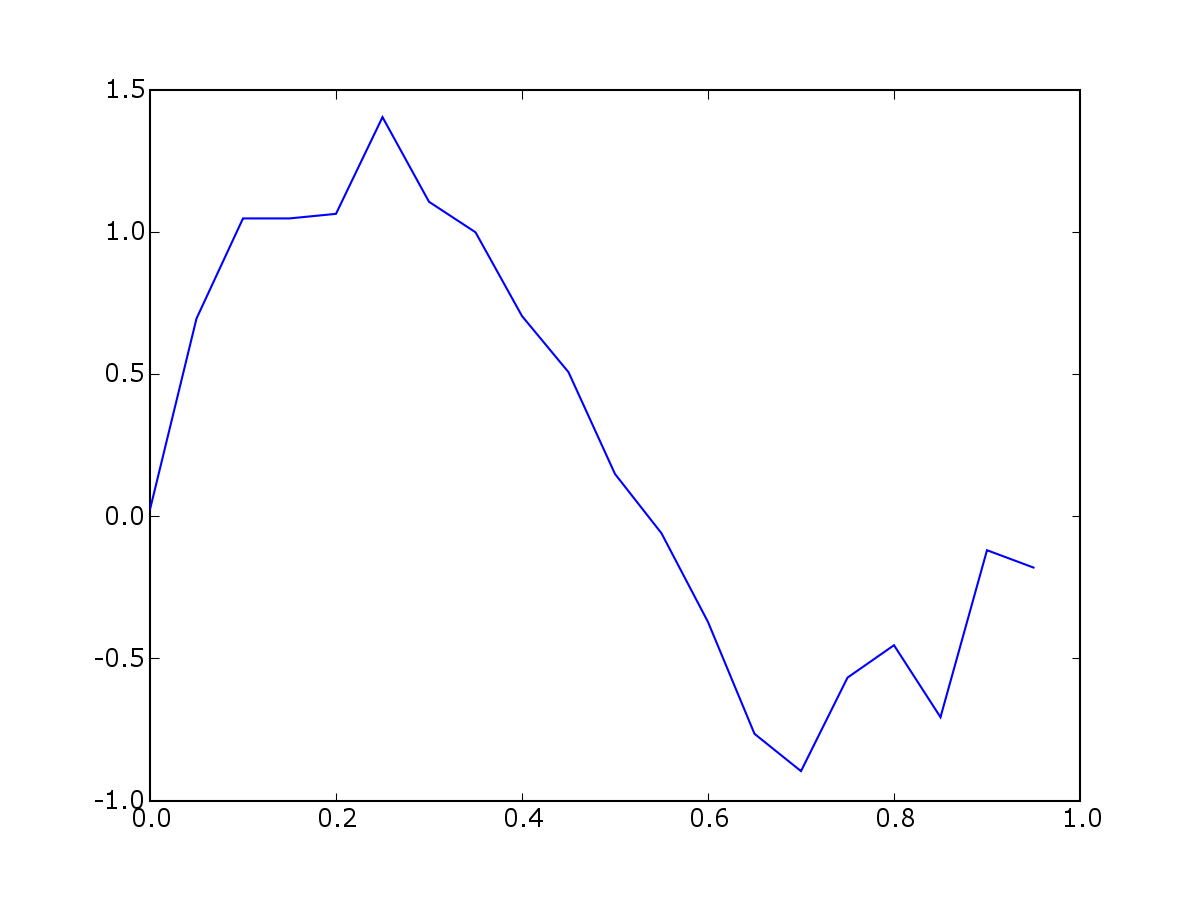
\includegraphics[width=4in]{fig/load_ascii}
\par\end{centering}

\caption{\label{fig:load_ascii}Loading \texttt{ASCII} data and displaying
with \texttt{plot}}

\end{figure}

\end{lyxcode}
\lstinputlisting[caption={Loading an ASCII text file and plotting the columns}]{snippets/load_data.ipy}



It is also easy to load data from binary files. In the example below,
we have some image data in raw binary string format. The image is
256x256 pixels, and each pixel is a 2 byte integer. We read this into
a string using python's \texttt{file} function -- the 'rb' flag says
to open the file in \texttt{read/binary} mode. We can then use the
numpy \texttt{fromstring} method to convert this to an array, passing
the type of the data (\texttt{int16}) as an argument. We reshape the
array by changing the array shape attribute to 256 by 256, and pass
this off to the matplotlib pylab command \texttt{imshow} for plotting.
matplotlib has a number of colormaps, and the default one is jet;
the data are automatically normalized and colormaps producing the
image in Figure \ref{fig:array_hothead}

\lstinputlisting[caption={Loading an binary image data and plotting it in matplotlib}]{snippets/load_binary.ipy}



%
\begin{figure}
\begin{centering}
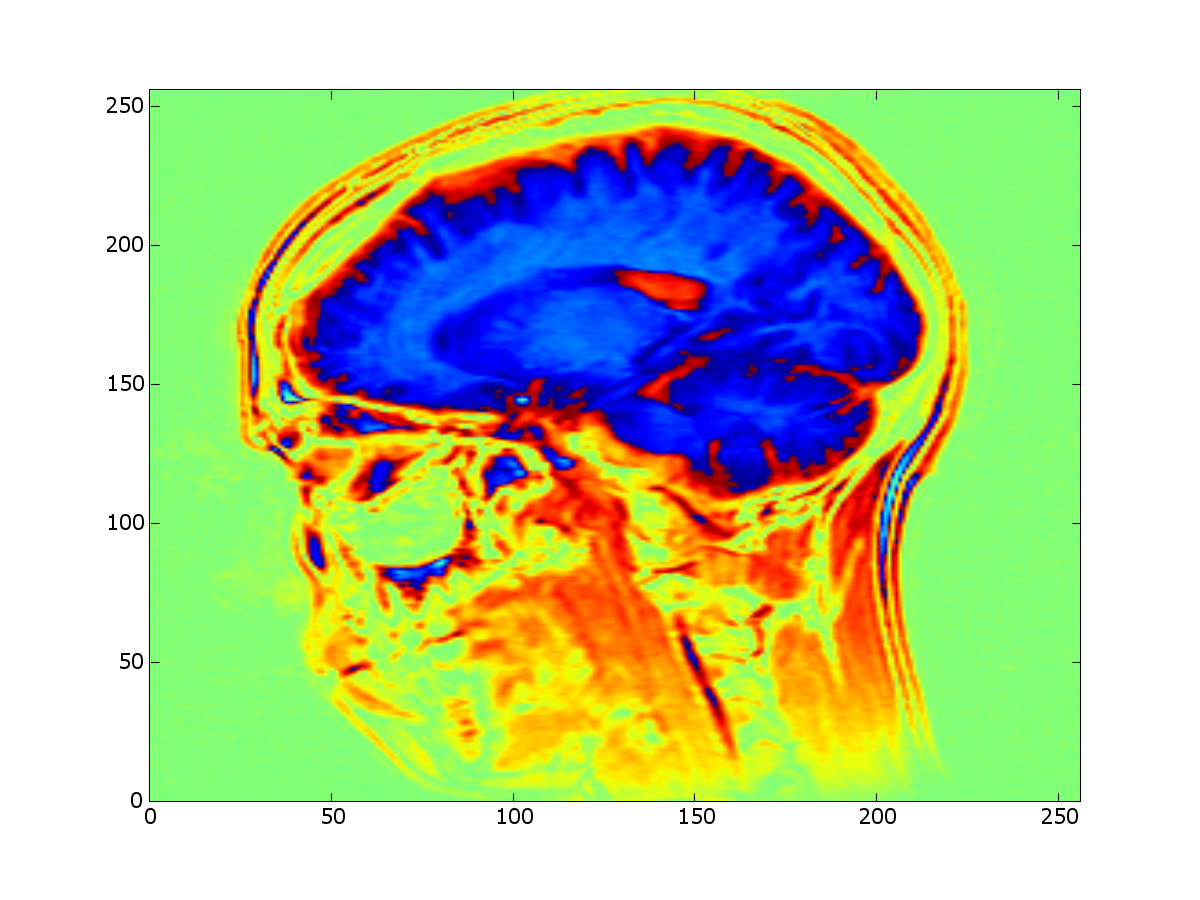
\includegraphics[width=4in]{fig/hothead}
\par\end{centering}

\caption{\label{fig:array_hothead}Loading binary image data and displaying
with \texttt{imshow}}

\end{figure}



\section[Arrays]{An Introduction to Arrays}


\subsection{Creating arrays}

There are a few different ways to create arrays besides modules that
obtain arrays from data files such

\begin{lyxcode}
>\,{}>\,{}>~x~=~zeros((20,30))
\end{lyxcode}
creates a 20x30 array of zeros (default integer type; details on how
to specify other types will follow). Note that the dimensions ({}``shape''
in numpy parlance) are specified by giving the dimensions as a
comma-separated list within parentheses. The parentheses aren't necessary
for a single dimension. As an aside, the parentheses used this way
are being used to specify a Python tuple; more will be said about
those in a later tutorial. For now you only need to imitate this usage.

Likewise one can create an array of 1's using the \texttt{ones()}
function.

The \texttt{arange()} function can be used to create arrays with sequential
values. E.g.,

\begin{lyxcode}
>\,{}>\,{}>~arange(10)

array({[}0,~1,~2,~3,~4,~5,~6,~7,~8,~9])
\end{lyxcode}
Note that that the array defaults to starting with a 0 value and does
not include the value specified (though the array does have a length
that corresponds to the argument)

Other variants:

\begin{lyxcode}
>\,{}>\,{}>~arange(10.)

array({[}~0.,~1.,~2.,~3.,~4.,~5.,~6.,~7.,~8.,~9])

>\,{}>\,{}>~arange(3,10)

array({[}3,~4,~5,~6,~7,~8,~9])

>\,{}>\,{}>~arange(1.,~10.,~1.1)~\#~note~trickiness

array({[}1.~,~2.1,~3.2,~4.3,~5.4,~6.5,~7.6,~8.7,~9.8])
\end{lyxcode}
Finally, one can create arrays from literal arguments:

\begin{lyxcode}
>\,{}>\,{}>~print~array({[}3,1,7])

{[}3~1~7]

>\,{}>\,{}>~print~array({[}{[}2,3],{[}4,4]])

{[}{[}2~3]

~{[}4~4]]
\end{lyxcode}
The brackets, like the parentheses in the zeros example above have
a special meaning in Python which will be covered later (Python lists).
For now, just mimic the syntax used here.


\subsection{Array numeric types}

numpy supports all standard numeric types. The default integer
matches what Python uses for integers, usually 32 bit integers or
what numpy calls \texttt{int32}. The same is true for floats, i.e.,
generally 64-bit doubles called \texttt{float64} in numpy. The
default complex type is \texttt{complex64}. Many of the functions
accept a type argument. For example

\begin{lyxcode}
>\,{}>\,{}>~zeros(3,~int8)~\#~Signed~byte

>\,{}>\,{}>~zeros(3,~dtype=uint8)~\#~Unsigned~byte

>\,{}>\,{}>~array({[}2,3],~dtype=float32)

>\,{}>\,{}>~arange(4,~dtype=complex64)
\end{lyxcode}
The possible types are \texttt{int8, uint8, int16, uint16, int32,
uint32, int64, uint64, float32, float64, complex32, complex64.} To
find out the type of an array use the .dtype() method. E.g.,

\begin{lyxcode}
>\,{}>\,{}>~arr.dtype()
dtype('float32')
\end{lyxcode}
To convert an array to a different type use the \texttt{astype()}
method, e.g,

\begin{lyxcode}
>\,{}>\,{}>~a~=~arr.astype(float64)
\end{lyxcode}

\subsection{Printing arrays}

Interactively, there are two common ways to see the value of an array.
Like many Python objects, just typing the name of the variable itself
will print its contents (this only works in interactive mode). You
can also explicitly print it. The following illustrates both approaches:

\begin{lyxcode}
>\,{}>\,{}>~x~=~arange(10)

>\,{}>\,{}>~x

array({[}0,~1,~2,~3,~4,~5,~6,~7,~8~9])

>\,{}>\,{}>~print~x

{[}0~1~2~3~4~5~6~7~8~9]
\end{lyxcode}
By default the array module limits the amount of an array that is
printed out (to spare you the effects of printing out millions of
values). For example:

\begin{lyxcode}
>\,{}>\,{}>~x~=~arange(1000000)

print~x

{[}~~~~0~~~~~1~~~~~2~...,~999997~999998~999999]
\end{lyxcode}

\subsection{Indexing 1-D arrays}

As with IDL and Matlab, there are many options for indexing arrays.

\begin{lyxcode}
>\,{}>\,{}>~x~=~arange(10)

>\,{}>\,{}>~x

array({[}0,~1,~2,~3,~4,~5,~6,~7,~8,~9])
\end{lyxcode}
Simple indexing:

\begin{lyxcode}
>\,{}>\,{}>~x{[}2]~\#~3rd~element

2
\end{lyxcode}
Indexing is 0-based. The first value in the array is \texttt{x{[}0]}

Indexing from end:

\begin{lyxcode}
>\,{}>\,{}>~x{[}-2]~\#~-1~represents~the~last~element,~-2~next~to~last...

8
\end{lyxcode}
Slices

To select a subset of an array:

\begin{lyxcode}
>\,{}>\,{}>~x{[}2:5]

array({[}2,~3,~4])
\end{lyxcode}
Note that the upper limit of the slice is not included as part of
the subset! This is viewed as unexpected by newcomers and a defect.
Most find this behavior very useful after getting used to it (the
reasons won't be given here). Also important to understand is that
slices are views into the original array in the same sense that references
view the same array. The following demonstrates:

\begin{lyxcode}
>\,{}>\,{}>~y~=~x{[}2:5]

>\,{}>\,{}>~y{[}0]~=~99

>\,{}>\,{}>~y

array({[}99,~3,~4])

>\,{}>\,{}>~x

array({[}0,~1,~99,~3,~4,~5,~6,~7,~8,~9])
\end{lyxcode}
Changes to a slice will show up in the original. If a copy is needed
use \texttt{x{[}2:5].copy()}

Short hand notation

\begin{lyxcode}
>\,{}>\,{}>~x{[}:5]~\#~presumes~start~from~beginning

array({[}~0,~1,~99,~3,~4])

>\,{}>\,{}>~x{[}2:]~\#~presumes~goes~until~end

array({[}99,~3,~4,~5,~6,~7,~8,~9])

>\,{}>\,{}>~x{[}:]~\#~selects~whole~dimension

array({[}0,~1,~99,~3,~4,~5,~6,~7,~8,~9])
\end{lyxcode}
Strides:

\begin{lyxcode}
>\,{}>\,{}>~x{[}2:8:3]~\#~Stride~every~third~element

array({[}99,~5])
\end{lyxcode}
Index arrays:

\begin{lyxcode}
>\,{}>\,{}>~x{[}{[}4,2,4,1]]

array({[}4,~99,~4,~1])
\end{lyxcode}
Using results of logical indexing 

\begin{lyxcode}
>\,{}>\,{}>~x~>~5

array({[}0,0,1,0,0,0,1,1,1,1],~type=Bool)

>\,{}>\,{}>~x{[}x>5]

array({[}99,~6,~7,~8,~9])
\end{lyxcode}

\subsection{Indexing multidimensional arrays}

Before describing this in detail it is very important to note an item
regarding multidimensional indexing that will certainly cause you
grief until you become accustomed to it: ARRAY INDICES USE THE OPPOSITE
CONVENTION AS FORTRAN REGARDING ORDER OF INDICES FOR MULTIDIMENSIONAL
ARRAYS.

\begin{lyxcode}
>\,{}>\,{}>~im~=~arange(24)

>\,{}>\,{}>~im.shape~=~4,6

>\,{}>\,{}>~im

array({[}{[}~0,~~1,~~2,~~3,~~4,~~5],

~~~~~~~{[}~6,~~7,~~8,~~9,~10,~11],

~~~~~~~{[}12,~13,~14,~15,~16,~17],

~~~~~~~{[}18,~19,~20,~21,~22,~23]])
\end{lyxcode}
To emphasize the point made in the previous paragraph, the index that
represents the most rapidly varying dimension in memory is the 2nd
index, not the first. 

Partial indexing:

\begin{lyxcode}
>\,{}>\,{}>~im{[}1]

array({[}6,~7,~8,~9,~10,~11])
\end{lyxcode}
If only some of the indices for a multidimensional array are specified,
then the result is an array with the shape of the {}``leftover''
dimensions, in this case, 1-dimensional. The 2nd row is selected,
and since there is no index for the column, the whole row is selected.

All of the indexing tools available for 1-D arrays apply to \emph{n}-dimensional
arrays as well (though combining index arrays with slices is not currently
permitted). To understand all the indexing options in their full detail,
read sections 4.6, 4.7 and 6 of the numpy manual.


\subsection{Compatibility of dimensions}

In operations involving combining (e.g., adding) arrays or assigning
them there are rules regarding the compatibility of the dimensions
involved. For example the following is permitted:

\begin{lyxcode}
>\,{}>\,{}>~x{[}:5]~=~0
\end{lyxcode}
since a single value is considered {}``broadcastable'' over a 5
element array. But this is not permitted:

\begin{lyxcode}
>\,{}>\,{}>~x{[}:5]~=~array({[}0,1,2,3])~
\end{lyxcode}
since a 4 element array does not match a 5 element array. 

\emph{The following explanation can probably be skipped by most on
the first reading;} it is only important to know that rules for combining
arrays of different shapes are quite general. It is hard to precisely
specify the rules without getting a bit confusing, but it doesn't
take long to get a good intuitive feeling for what is and isn't permitted.
Here's an attempt anyway: The shapes of the two involved arrays when
aligned on their trailing part must be equal in value or one must
have the value one for that dimension. The following pairs of shapes
are compatible:

\begin{lyxcode}
(5,4):(4,)~->~(5,4)

(5,1):(4,)~->~(5,4)

(15,3,5):(15,1,5)~->~(15,3,5)

(15,3,5):(3,5)~->~(15,3,5)

(15,1,5):(3,1)~->~(15,3,5)
\end{lyxcode}
so that one can add arrays of these shapes or assign one to the other
(in which case the one being assigned must be the smaller shape of
the two). For the dimensions that have a 1 value that are matched
against a larger number, the values in that dimension are simply repeated.
For dimensions that are missing, the sub-array is simply repeated
for those. The following shapes are not compatible:

\begin{lyxcode}
(3,4):(4,3)

(1,3):(4,)
\end{lyxcode}
Examples:

\begin{lyxcode}
>\,{}>\,{}>~x~=~zeros((5,4))

>\,{}>\,{}>~x{[}:,:]~=~{[}2,3,2,3]

>\,{}>\,{}>~x

array({[}{[}2,~3,~2,~3],

~~~~~~~{[}2,~3,~2,~3],

~~~~~~~{[}2,~3,~2,~3],

~~~~~~~{[}2,~3,~2,~3],

~~~~~~~{[}2,~3,~2,~3]])

>\,{}>\,{}>~a~=~arange(3)

>\,{}>\,{}>~b~=~a{[}:]~\#~different~array,~same~data~(huh?)

>\,{}>\,{}>~b.shape~=~(3,1)

>\,{}>\,{}>~b

array({[}{[}0],

~~~~~~~{[}1],

~~~~~~~{[}2]])

>\,{}>\,{}>~a{*}b~\#~outer~product

array({[}{[}0,~0,~0],

~~~~~~~{[}0,~1,~2],

~~~~~~~{[}0,~2,~4]])
\end{lyxcode}

\subsection{ufuncs}

A ufunc (short for Universal Function) applies the same operation
or function to all the elements of an array independently. When two
arrays are added together, the \texttt{add} ufunc is used to perform
the array addition. There are ufuncs for all the common operations
and mathematical functions. More specialized ufuncs can be obtained
from add-on libraries. All the operators have corresponding ufuncs
that can be used by name (e.g., \texttt{add} for \texttt{+}). These
are all listed in table below. Ufuncs also have a few very handy methods
for binary operators and functions whose use are demonstrated here.

\begin{lyxcode}
>\,{}>\,{}>~x~=~arange(9)

>\,{}>\,{}>~x.shape~=~(3,3)

>\,{}>\,{}>~x

array({[}0,~1,~2],

~~~~~~{[}3,~4,~5],

~~~~~~{[}6,~7,~8]])

>\,{}>\,{}>~add.reduce(x)~\#~sums~along~the~first~index

array({[}9,~12,~15])

>\,{}>\,{}>~add.reduce(x,~axis=1)~\#~sums~along~the~2nd~index

array({[}3,~12,~21])

>\,{}>\,{}>~add.accumulate(x)~\#~cumulative~sum~along~the~first~index

array({[}{[}0,~~1,~~2],

~~~~~~~{[}3,~~5,~~7],

~~~~~~~{[}9,~12,~15]])

>\,{}>\,{}>~multiply.outer(arange(3),arange(3))

array({[}{[}0,~0,~0],

~~~~~~~{[}0,~1,~2],

~~~~~~~{[}0,~2,~4]])
\end{lyxcode}
Standard Ufuncs (with corresponding symbolic operators, when they
exist, shown in parentheses)

\begin{tabular}{lll}
add (+) & log & greater (>)\tabularnewline
subtract (-) & log10 & greater\_equal (>=)\tabularnewline
multiply ({*}) & cos & less (<)\tabularnewline
divide (/) & arcos & less\_equal (<=)\tabularnewline
remainder (\%) & sin & logical\_and\tabularnewline
absolute, abs & arcsin & logical\_or\tabularnewline
floor & tan & logical\_xor\tabularnewline
ceil & arctan & bitwise\_and (\&)\tabularnewline
fmod & cosh & bitwise\_or (|)\tabularnewline
conjugate & sinh & bitwise\_xor (\textasciicircum{})\tabularnewline
minimum & tanh & bitwise\_not (\textasciitilde{})\tabularnewline
maximum & sqrt & rshift (>\,{}>)\tabularnewline
power ({*}{*}) & equal (==) & lshift (<\,{}<)\tabularnewline
exp & not\_equal (!=) & \tabularnewline
 &  & \tabularnewline
\end{tabular}

\emph{Note that there are no corresponding Python operators for} \texttt{logical\_and}
\emph{and} \texttt{logical\_or}\emph{. The Python} \texttt{and} \emph{and}
\texttt{or} \emph{operators are NOT equivalent to these respective
ufuncs!}


\subsection{Array functions}

There are many array utility functions. The following lists the more
useful ones with a one line description. See the numpy manual for
details on how they are used. Arguments shown with argument=value
indicate what the default value is if called without a value for that
argument.

\begin{description}
\item [{\texttt{all}\textmd{(}\textmd{\emph{a}}\textmd{):}}] are all elements
of array nonzero
\item [{\texttt{allclose}\textmd{(}\textmd{\emph{a1,~a2,~rtol=1.e-5,~atol=1.e-8}}\textmd{):}}] true
if all elements within specified amount (between two arrays)
\begin{spacing}{0.50}
\item [{\texttt{alltrue}\textmd{(}\textmd{\emph{a,~axis=0}}\textmd{):}}] are
all elements nonzero along specified axis true.\end{spacing}

\item [{\texttt{any}\textmd{(}\textmd{\emph{a}}\textmd{):}}] are any elements
of an array nonzero
\begin{spacing}{0.50}
\item [{\texttt{argmax}\textmd{(}\textmd{\emph{a,~axis=-1}}\textmd{),~argmin(}\textmd{\emph{a,axis=-1}}\textmd{):}}] return
array with min/max locations for selected axis
\item [{\texttt{argsort}\textmd{(}\textmd{\emph{a,~axis=-1}}\textmd{):}}] returns
indices of results of sort on an array
\item [{\texttt{choose}\textmd{(}\textmd{\emph{selector,~population,~clipmode=CLIP}}\textmd{):}}] fills
specified array by selecting corresponding values from a set of arrays
using integer selection array (population is a tuple of arrays; see
tutorial 2)
\item [{\texttt{clip}\textmd{(}\textmd{\emph{a,~amin,~amax}}\textmd{):}}] clip
values of array \emph{a} at values \emph{amin}, \emph{amax}
\item [{\texttt{dot}\textmd{(}\textmd{\emph{a1,~a2}}\textmd{):}}] dot
product of arrays \texttt{\emph{a1}} \& \texttt{\emph{a2}}
\item [{\texttt{compress}\textmd{(}\textmd{\emph{condition,~a~,axis=0}}\textmd{):}}] selects
elements from array \emph{a} based on boolean arraycondition
\item [{\texttt{concatenate}\textmd{(}\textmd{\emph{arrays,~axis=0}}\textmd{):}}] concatenate
arrays contained in sequence of arrays arrays
\item [{\texttt{cumproduct}\textmd{(}\textmd{\emph{a,~axis=0}}\textmd{):}}] net
cumulative product along specified axis
\item [{\texttt{cumsum}\textmd{(}\textmd{\emph{a,~axis=0}}\textmd{):}}] accumulate
array along specified axis
\item [{\texttt{diagonal}\textmd{(}\textmd{\emph{a,~offset=0,~axis1=0,~axis2=1}}\textmd{):}}] returns
diagonal of 2-d matrix with optional offsets. \end{spacing}

\item [{\texttt{fromfile}\textmd{(}\textmd{\emph{file,~type,~shape=None}}\textmd{):}}] Use
binary data in file to form new array of specified type.
\item [{\texttt{fromstring}\textmd{(}\textmd{\emph{datastring,~type,~shape=None}}\textmd{):}}] Use
binary data in \emph{datastring} to form new array of specified shape
and type
\item [{\texttt{identity}\textmd{(}\textmd{\emph{n,~type=None}}\textmd{):}}] returns
identity matrix of size nxn.
\begin{spacing}{0.50}
\item [{\texttt{indices}\textmd{(}\textmd{\emph{shape,~type=None}}\textmd{):}}] generate
array with values corresponding to position of selected index of the
array
\item [{\texttt{innerproduct}\textmd{(}\textmd{\emph{a1,~a2}}\textmd{):}}] guess
\item [{\texttt{matrixmultiply}\textmd{(}\textmd{\emph{a1,~a2}}\textmd{):}}] guess
\item [{\texttt{outerproduct}\textmd{(}\textmd{\emph{a1,~a2}}\textmd{):}}] guess
\item [{\texttt{product}\textmd{(}\textmd{\emph{a,~axis=0}}\textmd{):}}] net
product of elements along specified axis
\item [{\texttt{ravel}\textmd{(}\textmd{\emph{a}}\textmd{):}}] creates
a 1-d version of an array
\item [{\texttt{repeat}\textmd{(}\textmd{\emph{a,~repeats,~axis=0}}\textmd{):}}] generates
new array with repeated copies of input array \emph{a}
\item [{\texttt{resize}\textmd{(}\textmd{\emph{a,~shape}}\textmd{):}}] replicate
or truncate array to new shape
\item [{\texttt{searchsorted}\textmd{(}\textmd{\emph{bin,~a}}\textmd{):}}] return
indices of mapping values of an array \emph{a} into a monotonic array
\emph{bin}
\item [{\texttt{sometrue}\textmd{(}\textmd{\emph{a,~axis=0}}\textmd{):}}] are
any elements along specified axis true 
\item [{\texttt{sort}\textmd{(}\textmd{\emph{a,~axis=-1}}\textmd{):}}] sort
array elements along selected axis
\item [{\texttt{sum}\textmd{(}\textmd{\emph{a,~axis=0}}\textmd{):}}] sum
array along specified axis
\item [{\texttt{swapaxes}\textmd{(}\textmd{\emph{a,~axis1,~axis2}}\textmd{):}}] switch
indices for axis of array (doesn't actually move data, just maps indices
differently)
\item [{\texttt{trace}\textmd{(}\textmd{\emph{a,~offset=0,~axis1=0,~axis2=1}}\textmd{):}}] compute
trace of matrix \emph{a} with optional offset.
\item [{\texttt{transpose}\textmd{(}\textmd{\emph{a,~axes=None}}\textmd{):}}] transpose
indices of array (doesn't actually move data, just maps indices differently)\end{spacing}

\item [{\texttt{where}\textmd{(}\textmd{\emph{a}}\textmd{):}}] find {}``true''
locations in array \emph{a}
\end{description}

\subsection{Array methods}

\begin{singlespace}
Arrays have several methods. They are used as methods are with any
object. For example (using the array from the previous example):
\end{singlespace}

\begin{lyxcode}
\begin{singlespace}
>\,{}>\,{}>~\#~sum~all~array~elements

>\,{}>\,{}>~x.sum()~\#~the~L~indicates~a~Python~Long~integer

36L~\end{singlespace}

\end{lyxcode}
\begin{singlespace}
The following lists all the array methods that exist for an array
object \texttt{a} (a number are equivalent to array functions; these
have no summary description shown):
\end{singlespace}

\begin{description}
\begin{spacing}{0.50}
\item [{\texttt{\emph{a}}\texttt{.argmax}\textmd{(}\textmd{\emph{axis=-1}})}]~
\item [{\texttt{\emph{a}}\texttt{.argmin}\textmd{(}\textmd{\emph{axis=-1}})}]~
\item [{\texttt{\emph{a}}\texttt{.argsort}\textmd{(}\textmd{\emph{axis=-1}})}]~
\item [{\texttt{\emph{a}}\texttt{.astype}\textmd{(}\textmd{\emph{type}}\textmd{):}}] copy
array to specified numeric type
\item [{\texttt{\emph{a}}\texttt{.byteswap}\textmd{():}}] perform byteswap
on data in place
\item [{\texttt{\emph{a}}\texttt{.byteswapped}\textmd{():}}] return byteswapped
copy of array
\item [{\texttt{\emph{a}}\texttt{.conjugate}\textmd{():}}] complex conjugate
\item [{\texttt{\emph{a}}\texttt{.copy}\textmd{():}}] produce copied version
of array (instead of view)
\item [{\texttt{\emph{a}}\texttt{.diagonal}\textmd{()}}]~
\item [{\texttt{\emph{a}}\texttt{.info}\textmd{():}}] print info about
array
\item [{\texttt{\emph{a}}\texttt{.isaligned}\textmd{():}}] are data elements
guaranteed aligned with memory?
\item [{\texttt{\emph{a}}\texttt{.isbyteswapped}\textmd{():}}] are data
elements in native processor order?
\item [{\texttt{\emph{a}}\texttt{.iscontiguous}\textmd{():}}] are data
elements contiguous in memory?
\item [{\texttt{\emph{a}}\texttt{.is\_c\_array}\textmd{():}}] are data
elements aligned, not byteswapped, and contiguous?
\item [{\texttt{\emph{a}}\texttt{.is\_fortran\_contiguous}\textmd{():}}] are
indicies defined to follow Fortran conventions?
\item [{\texttt{\emph{a}}\texttt{.is\_f\_array}\textmd{():}}] are indices
defined to follow Fortran conventions and data are aligned and not
byteswapped
\item [{\texttt{\emph{a}}\texttt{.itemsize}\textmd{():}}] size of data
element in bytes
\item [{\texttt{\emph{a}}\texttt{.max}\textmd{(type=None):}}] maximum value
in array
\item [{\texttt{\emph{a}}\texttt{.min}\textmd{():}}] minimum value in array
\item [{\texttt{\emph{a}}\texttt{.nelements}\textmd{():}}] total number
of elements in array
\item [{\texttt{\emph{a}}\texttt{.new}\textmd{():}}] returns new array
of same type and size (data uninitialized)
\item [{\texttt{\emph{a}}\texttt{.repeat}\textmd{(a,repeats,axis=0):}}]~
\item [{\texttt{\emph{a}}\texttt{.resize}\textmd{(shape):}}]~
\item [{\texttt{\emph{a}}\texttt{.size}\textmd{():}}] same as nelements
\item [{\texttt{\emph{a}}\texttt{.dtype}\textmd{():}}] returns type of array
\item [{\texttt{\emph{a}}\texttt{.tofile}\textmd{(}\textmd{\emph{file}}\textmd{):}}] write
binary data to file
\item [{\texttt{\emph{a}}\texttt{.tolist}\textmd{():}}] convert data to
Python list format
\item [{\texttt{\emph{a}}\texttt{.tostring}\textmd{():}}] copy binary data
to Python string
\item [{\texttt{\emph{a}}\texttt{.transpose}\textmd{(}\textmd{\emph{axes=-1}}\textmd{):}}] transpose
array
\item [{\texttt{\emph{a}}\texttt{.stddev}\textmd{():}}] standard deviation
\item [{\texttt{\emph{a}}\texttt{.sum}\textmd{():}}] sum of all elements
\item [{\texttt{\emph{a}}\texttt{.swapaxes}\textmd{(}\textmd{\emph{axis1,axis2}})}]~
\item [{\texttt{\emph{a}}\texttt{.togglebyteorder}\textmd{():}}] change
byteorder flag without changing actual data byteorder
\item [{\texttt{\emph{a}}\texttt{.trace}\textmd{()}}]~
\item [{\texttt{\emph{a}}\texttt{.view}\textmd{():}}] returns new array
object using view of same data\end{spacing}

\end{description}

\subsection{Array attributes:}

\begin{description}
\begin{spacing}{0.50}
\item [{\texttt{a.shape:}}] returns shape of array
\item [{\texttt{a.flat:}}] returns view of array treating it as 1-dimensional.
Doesn't work if array is not contiguous
\item [{\texttt{a.real:}}] return real component of array (exists for all
types)
\item [{\texttt{a.imag,~a.imaginary:}}] return imaginary component (exists
only for complex types)\end{spacing}

\end{description}

\section{Exercises}

\begin{xca}
Load the binary image shown in Figure\ref{fig:array_hothead}. What
is the mean pixel value, what are the standard deviation of pixel
values? Sum over the rows and make a bar plot for the summated intensity
across rows. Do the same for columns. Make a histogram of all the
data in the image. (Hint -- see n\texttt{x.mlab.mean}, \texttt{nx.mlab.std},
\texttt{pylab.bar} and \texttt{pylab.hist)}
\end{xca}
\begin{example}
this is another test
\end{example}
this is a test



\chapter[Python intro]{A whirlwind tour of python and the standard library}

This is a quick-and-dirty introduction to the python language for
the impatient scientist. There are many top notch, comprehensive introductions
and tutorials for python. For absolute beginners, there is the \textit{Python
Beginner's Guide}.%
\footnote{http://www.python.org/moin/BeginnersGuide%
} The official \textit{Python Tutorial} can be read online%
\footnote{http://docs.python.org/tut/tut.html%
} or downloaded%
\footnote{http://docs.python.org/download.html%
} in a variety of formats. There are over 100 python tutorials collected
online.%
\footnote{http://www.awaretek.com/tutorials.html%
}

There are also many excellent books. Targetting newbies is Mark Pilgrim's
\textit{Dive into Python} which in available in print and for free
online%
\footnote{http://diveintopython.org/toc/index.html%
}, though for absolute newbies even this may be too hard \cite{Dive}.
For experienced programmers, David Beasley's \textit{Python Essential
Reference} is an excellent introduction to python, but is a bit dated
since it only covers python2.1 \cite{Beasley}. Likwise Alex Martelli's
\textit{Python in a Nutshell} is highly regarded and a bit more current
-- a 2nd edition is in the works\cite{Nutshell}. And \textit{The
Python Cookbook} is an extremely useful collection of python idioms,
tips and tricks \cite{Cookbook}.

But the typical scientist I encounter wants to solve a specific problem,
eg, to make a certain kind of graph, to numerically integrate an equation,
or to fit some data to a parametric model, and doesn't have the time
or interest to read several books or tutorials to get what they want.
This guide is for them: a short overview of the language to help them
get to what they want as quickly as possible. We get to advanced material
pretty quickly, so it may be touch sledding if you are a python newbie.
Take in what you can, and if you start getting dizzy, skip ahead to
the next section; you can always come back to absorb more detail later,
after you get your real work done.


\section{Hello Python}

Python is a dynamically typed, object oriented, interpreted language.
Interpreted means that your program interacts with the python interpreter,
similar to Matlab, Perl, Tcl and Java, and unlike FORTRAN, C, or C++
which are compiled. So let's fire up the python interpreter and get
started. I'm not going to cover installing python -- it's standard
on most linux boxes and for windows there is a friendly GUI installer.
To run the python interpreter, on windows, you can click \texttt{Start->All
Programs->Python 2.4->Python (command line)} or better yet, install
\texttt{ipython}, a python shell on steroids, and use that. On linux
/ unix systems, you just need to type \texttt{python} or \texttt{ipython}
at the command line. The \texttt{>\,{}>\,{}>} is the default python
shell prompt, so don't type it in the examples below

\begin{lyxcode}
>\,{}>\,{}>~print~'hello~world'

hello~world


\end{lyxcode}
As this example shows, \textit{hello world} in python is pretty easy
-- one common phrase you hear in the python community is that {}``it
fits your brain''. -- the basic idea is that coding in python feels
natural. Compare python's version with \textit{hello world} in C++

\begin{lyxcode}
//~C++

\#include~<iostream>

int~main~()

\{~~~

~~std::cout~<\,{}<~\char`\"{}Hello~World\char`\"{}~<\,{}<~std::endl;

~~return~0;

\}
\end{lyxcode}

\section[Calculator]{\label{sec:into_calculator}Python is a calculator}

Aside from my daughter's solar powered cash-register calculator, Python
is the only calculator I use. From the python shell, you can type
arbitrary arithmetic expressions.

\begin{lyxcode}
>\,{}>\,{}>~2+2

4

>\,{}>\,{}>~2{*}{*}10

1024

>\,{}>\,{}>~10/5

2

>\,{}>\,{}>~2+(24.3~+~.9)/.24

107.0

>\,{}>\,{}>~2/3

0
\end{lyxcode}
The last line is a standard newbie gotcha -- if both the left and
right operands are integers, python returns an integer. To do floating
point division, make sure at least one of the numbers is a float

\begin{lyxcode}
>\,{}>\,{}>~2.0/3

0.66666666666666663
\end{lyxcode}
The distinction between integer and floating point division is a common
source of frustration among newbies and is slated for destruction
in the mythical Python 3000.%
\footnote{Python 3000 is a future python release that will clean up several
things that Guido considers to be warts.%
} Since default integer division will be removed in the future, you
can invoke the time machine with the \texttt{from \_\_future\_\_}
directives; these directives allow python programmers today to use
features that will become standard in future releases but are not
included by default because they would break existing code. From future
directives should be among the first lines you type in your python
code if you are going to use them, otherwise they may not work. The
future division operator will assume floating point division by default,%
\footnote{You may have noticed that 2/3 was represented as 0.66666666666666663
and not 0.66666666666666666 as might be expected. This is because
computers are binary calculators, and there is no exact binary representation
of 2/3, just as there is no exact binary representation of 0.1

\begin{lyxcode}
>\,{}>\,{}>~0.1

0.10000000000000001
\end{lyxcode}
Some languages try and hide this from you, but python is explicit.%
}and provides another operator // to do classic integer division.

\begin{lyxcode}
>\,{}>\,{}>~from~\_\_future\_\_~import~division

>\,{}>\,{}>~2/3

0.66666666666666663

>\,{}>\,{}>~2//3

0
\end{lyxcode}
python has four basic numeric types: int, long, float and complex,
but unlike C++, BASIC, FORTRAN or Java, you don't have to declare
these types. python can infer them

\begin{lyxcode}
>\,{}>\,{}>~type(1)

<type~'int'>

>\,{}>\,{}>~type(1.0)

<type~'float'>

>\,{}>\,{}>~type(2{*}{*}200)

<type~'long'>


\end{lyxcode}
$2^{200}$is a huge number!

\begin{lyxcode}
>\,{}>\,{}>~2{*}{*}200

1606938044258990275541962092341162602522202993782792835301376L
\end{lyxcode}
but python will blithely compute it and much larger numbers for you
as long as you have CPU and memory to handle them. The integer type,
if it overflows, will automatically convert to a python \texttt{long}
(as indicated by the appended \texttt{L} in the output above) and
has no built-in upper bound on size, unlike C/C++ longs.

Python has built in support for complex numbers. Eg, we can verify
$i^{2}=-1$ 

\begin{lyxcode}
>\,{}>\,{}>~x~=~complex(0,1)

>\,{}>\,{}>~x{*}x

(-1+0j)
\end{lyxcode}
To access the real and imaginary parts of a complex number, use the
\texttt{real} and \texttt{imag} attributes

\begin{lyxcode}
>\,{}>\,{}>~x.real

0.0

>\,{}>\,{}>~x.imag

1.0
\end{lyxcode}
If you come from other languages like Matlab, the above may be new
to you. In matlab, you might do something like this (>\,{}> is the
standard matlab shell prompt)

\begin{lyxcode}
>\,{}>~x~=~0+j

x~=

~~~0.0000~+~1.0000i



>\,{}>~real(x)

ans~=

~~~~~0



>\,{}>~imag(x)

ans~=

~~~~~1




\end{lyxcode}
That is, in Matlab, you use a \textit{function} to access the real
and imaginary parts of the data, but in python these are attributes
of the complex object itself. This is a core feature of python and
other object oriented languages: an object carries its data and methods
around with it. One might say: {}``a complex number knows it's real
and imaginary parts'' or {}``a complex number knows how to take
its conjugate'', you don't need external functions for these operations

\begin{lyxcode}
>\,{}>\,{}>~x.conjugate

<built-in~method~conjugate~of~complex~object~at~0xb6a62368>

>\,{}>\,{}>~x.conjugate()

-1j
\end{lyxcode}
On the first line, I just followed along from the example above with
\texttt{real} and \texttt{imag} and typed \texttt{x.conjugate} and
python printed the representation \texttt{<built-in method conjugate
of complex object at 0xb6a62368>.} This means that \texttt{conjugate}
is a \textit{method}, a.k.a a function, and in python we need to use
parentheses to call a function. If the method has arguments, like
the \texttt{x} in \texttt{sin(x)}, you place them inside the parentheses,
and if it has no arguments, like \texttt{conjugate}, you simply provide
the open and closing parentheses. \texttt{real}, \texttt{imag} and
\texttt{conjugate} are attributes of the complex object, and \texttt{conjugate}
is a \textit{callable} attribute, known as a \textit{method}.

OK, now you are an object oriented programmer. There are several key
ideas in object oriented programming, and this is one of them: an
object carries around with it data (simple attributes) and methods
(callable attributes) that provide additional information about the
object and perform services. It's one stop shopping -- no need to
go to external functions and libraries to deal with it -- the object
knows how to deal with itself.


\section[Standard Library]{Accessing the standard library}

Arithmetic is fine, but before long you may find yourself tiring of
it and wanting to compute logarithms and exponents, sines and cosines

\begin{lyxcode}
>\,{}>\,{}>~log(10)

Traceback~(most~recent~call~last):

~~File~\char`\"{}<stdin>\char`\"{},~line~1,~in~?

NameError:~name~'log'~is~not~defined
\end{lyxcode}
These functions are not built into python, but don't despair, they
are built into the python standard library. To access a function from
the standard library, or an external library for that matter, you
must import it.

\begin{lyxcode}
>\,{}>\,{}>~import~math

>\,{}>\,{}>~math.log(10)

2.3025850929940459

>\,{}>\,{}>~math.sin(math.pi)

1.2246063538223773e-16
\end{lyxcode}
Note that the default \texttt{log} function is a base 2 logarithm
(use \texttt{math.log10} for base 10 logs) and that floating point
math is inherently imprecise, since analytically$\sin(\pi)=0$.

It's kind of a pain to keep typing \texttt{math.log} and \texttt{math.sin}
and \texttt{math.p}i, and python is accomodating. There are additional
forms of \texttt{import} that will let you save more or less typing
depending on your desires

\begin{lyxcode}
\textcolor{blue}{\#~Appreviate~the~module~name:~m~is~an~alias}

>\,{}>\,{}>~import~math~as~m

>\,{}>\,{}>~m.cos(2{*}m.pi)

1.0



\textcolor{blue}{\#~Import~just~the~names~you~need}

>\,{}>\,{}>~from~math~import~exp,~log

>\,{}>\,{}>~log(exp(1))

1.0



\textcolor{blue}{\#~Import~everything~-~use~with~caution!}

>\,{}>\,{}>~from~math~import~{*}

>\,{}>\,{}>~sin(2{*}pi{*}10)

-2.4492127076447545e-15
\end{lyxcode}
To help you learn more about what you can find in the math library,
python has nice introspection capabilities -- introspection is a way
of asking an object about itself. For example, to find out what is
available in the math library, we can get a directory of everything
available with the \texttt{dir} command%
\footnote{In addition to the introdpection and help provided in the python interpreter,
the official documentation of the python standard library is very
good and up-to-date http://docs.python.org/lib/lib.html .%
}

\begin{lyxcode}
>\,{}>\,{}>~dir(math)

{[}'\_\_doc\_\_',~'\_\_file\_\_',~'\_\_name\_\_',~'acos',~'asin',~'atan',~'atan2',~'ceil',~'cos',~'cosh',~'degrees',~'e',~'exp',~'fabs',~'floor',~'fmod',~'frexp',~'hypot',~'ldexp',~'log',~'log10',~'modf',~'pi',~'pow',~'radians',~'sin',~'sinh',~'sqrt',~'tan',~'tanh']
\end{lyxcode}
This gives us just a listing of the names that are in the math module
-- they are fairly self descriptive, but if you want more, you can
call \texttt{help} on any of these functions for more information

\begin{lyxcode}
>\,{}>\,{}>~help(math.sin)~

Help~on~built-in~function~sin:

sin(...)

sin(x)

Return~the~sine~of~x~(measured~in~radians).
\end{lyxcode}
and for the whole math library

\begin{lyxcode}
>\,{}>\,{}>~help(math)~

Help~on~module~math:

~

NAME

~~~~math

~

FILE

~~~~/usr/local/lib/python2.3/lib-dynload/math.so

~

DESCRIPTION

~~~~This~module~is~always~available.~~It~provides~access~to~the

~~~~mathematical~functions~defined~by~the~C~standard.

~

FUNCTIONS

~~~~acos(...)

~~~~~~~~acos(x)

~~~~~~~~~

~~~~~~~~Return~the~arc~cosine~(measured~in~radians)~of~x.

~~~~~

~~~~asin(...)

~~~~~~~~asin(x)

~~~~~~~~~

~~~~~~~~Return~the~arc~sine~(measured~in~radians)~of~x.

~~~~~
\end{lyxcode}
And much more which is snipped. Likewise, we can get information on
the complex object in the same way

\begin{lyxcode}
>\,{}>\,{}>~x~=~complex(0,1)

>\,{}>\,{}>~dir(x)

{[}'\_\_abs\_\_',~'\_\_add\_\_',~'\_\_class\_\_',~'\_\_coerce\_\_',~'\_\_delattr\_\_',~'\_\_div\_\_',~'\_\_divmod\_\_',~'\_\_doc\_\_',~'\_\_eq\_\_',~'\_\_float\_\_',~'\_\_floordiv\_\_',~'\_\_ge\_\_',~'\_\_getattribute\_\_',~'\_\_getnewargs\_\_',~'\_\_gt\_\_',~'\_\_hash\_\_',~'\_\_init\_\_',~'\_\_int\_\_',~'\_\_le\_\_',~'\_\_long\_\_',~'\_\_lt\_\_',~'\_\_mod\_\_',~'\_\_mul\_\_',~'\_\_ne\_\_',~'\_\_neg\_\_',~'\_\_new\_\_',~'\_\_nonzero\_\_',~'\_\_pos\_\_',~'\_\_pow\_\_',~'\_\_radd\_\_',~'\_\_rdiv\_\_',~'\_\_rdivmod\_\_',~'\_\_reduce\_\_',~'\_\_reduce\_ex\_\_',~'\_\_repr\_\_',~'\_\_rfloordiv\_\_',~'\_\_rmod\_\_',~'\_\_rmul\_\_',~'\_\_rpow\_\_',~'\_\_rsub\_\_',~'\_\_rtruediv\_\_',~'\_\_setattr\_\_',~'\_\_str\_\_',~'\_\_sub\_\_',~'\_\_truediv\_\_',~'conjugate',~'imag',~'real']


\end{lyxcode}
Notice that called \texttt{dir} or \texttt{help} on the \texttt{math}
\textit{module}, the \texttt{math.sin} \textit{function}, and the
\texttt{complex} \textit{number} \texttt{x}. That's because modules,
functions and numbers are all \textit{objects}, and we use the same
object introspection and help capabilites on them. We can find out
what type of object they are by calling \texttt{type} on them, which
is another function in python's introspection arsenal

\begin{lyxcode}
>\,{}>\,{}>~type(math)

<type~'module'>

>\,{}>\,{}>~type(math.sin)

<type~'builtin\_function\_or\_method'>

>\,{}>\,{}>~type(x)

<type~'complex'>


\end{lyxcode}
Now, you may be wondering: what were all those god-awful looking double
underscore methods, like \texttt{\_\_abs\_\_} and \texttt{\_\_mul\_\_}
in the \texttt{dir} listing of the complex object above? These are
methods that define what it means to be a numeric type in python,
and the complex object implements these methods so that complex numbers
act like the way should, eg \texttt{\_\_mul\_\_} implements the rules
of complex multiplication. The nice thing about this is that python
specifies an application programming interface (API) that is the definition
of what it means to be a number in python. And this means you can
define your own numeric types, as long as you implement the required
special double underscore methods for your custom type. double underscore
methods are very important in python; although the typical newbie
never sees them or thinks about them, they are there under the hood
providing all the python magic, and more importantly, showing the
way to let you make magic.


\section{\label{sec:intro_string}Strings}

We've encountered a number of types of objects above: int, float,
long, complex, method/function and module. We'll continue our tour
with an introduction to strings, which are critical components of
almost every program. You can create strings in a number of different
ways, with single quotes, double quotes, or triple quotes -- this
diversity of methods makes it easy if you need to embed string characters
in the string itself

\begin{lyxcode}
\textcolor{blue}{\#~single,~double~and~triple~quoted~strings}

>\,{}>\,{}>~s~=~'Hi~Mom!'

>\,{}>\,{}>~s~=~\char`\"{}Hi~Mom!\char`\"{}

>\,{}>\,{}>~s~=~\char`\"{}\char`\"{}\char`\"{}Porky~said,~\char`\"{}That's~all~folks!\char`\"{}~\char`\"{}\char`\"{}\char`\"{}
\end{lyxcode}
You can add strings together to concatenate them

\begin{lyxcode}
\textcolor{blue}{\#~concatenating~strings}

>\,{}>\,{}>~first~=~'John'

>\,{}>\,{}>~last~=~'Hunter'

>\,{}>\,{}>~first+last

'JohnHunter'
\end{lyxcode}
or call string methods to process them: upcase them or downcase them,
or replace one character with another

\begin{lyxcode}
\textcolor{blue}{\#~string~methods}

>\,{}>\,{}>~last.lower()

'hunter'

>\,{}>\,{}>~last.upper()

'HUNTER'

>\,{}>\,{}>~last.replace('h',~'p')

'Hunter'

>\,{}>\,{}>~last.replace('H',~'P')

'Punter'~
\end{lyxcode}
Note that in all of these examples, the string \texttt{last} is unchanged.
All of these methods operate on the string and return a new string,
leaving the original unchanged. In fact, python strings cannot be
changed by any python code at all: they are \textit{immutable} (unchangeable).
The concept of mutable and immutable objects in python is an important
one, and it will come up again, because only immutable objects can
be used as keys in python dictionaries and elements of python sets.

You can access individual characters, or slices of the string (substrings),
using indexing. A string in sequence of characters, and strings implement
the sequence protocol in python -- we'll see more examples of python
sequences later -- and all sequences have the same syntax for accessing
their elements. Python uses 0 based indexing which means the first
element is at index 0; you can use negative indices to access the
last elements in the sequence

\begin{lyxcode}
\textcolor{blue}{\#~string~indexing}

>\,{}>\,{}>~last~=~'Hunter'

>\,{}>\,{}>~last{[}0]

'H'

>\,{}>\,{}>~last{[}1]

'u'

>\,{}>\,{}>~last{[}-1]~

'r'~
\end{lyxcode}
To access substrings, or generically in terms of the sequence protocol,
slices, you use a colon to indicate a range

\begin{lyxcode}
\textcolor{blue}{\#~string~slicing}

>\,{}>\,{}>~last{[}0:2]

'Hu'

>\,{}>\,{}>~last{[}2:4]

'nt'
\end{lyxcode}
As this example shows, python uses {}``one-past-the-end'' indexing
when defining a range; eg, in the range \texttt{indmin:indmax}, the
element of \texttt{imax} is not included. You can use negative indices
when slicing too; eg, to get everything before the last character

\begin{lyxcode}
>\,{}>\,{}>~last{[}0:-1]

'Hunte'
\end{lyxcode}
You can also leave out either the min or max indicator; if they are
left out, 0 is assumed to be the \texttt{indmin} and one past the
end of the sequence is assumed to be \texttt{indmax}

\begin{lyxcode}
>\,{}>\,{}>~last{[}:3]

'Hun'

>\,{}>\,{}>~last{[}3:]

'ter'
\end{lyxcode}
There is a third number that can be placed in a slice, a step, with
syntax indmin:indmax:step; eg, a step of 2 will skip every second
letter

\begin{lyxcode}
>\,{}>\,{}>~last{[}1:6:2]

'utr'
\end{lyxcode}
Although this may be more that you want to know about slicing strings,
the time spent here is worthwhile. As mentioned above, all python
sequences obey these rules. In addition to strings, lists and tuples,
which are built-in python sequence data types and are discussed in
the next section, the numeric arrays widely used in scientific computing
also implement the sequence protocol, and thus have the same slicing
rules.

\begin{xca}
What would you expect last{[}:] to return?
\end{xca}
One thing that comes up all the time is the need to create strings
out of other strings and numbers, eg to create filenames from a combination
of a base directory, some base filename, and some numbers. Scientists
like to create lots of data files like and then write code to loop
over these files and analyze them. We're going to show how to do that,
starting with the newbie way and progressively building up to the
way of python zen master. All of the methods below \textit{work},
but the zen master way will more efficient, more scalable (eg to larger
numbers of files) and cross-platform.%
\footnote{{}``But it works'' is a common defense of bad code; my rejoinder
to this is {}``A computer scientist is someone who fixes things that
aren't broken''. %
} Here's the newbie way: we also introduce the for-loop here in the
spirit of diving into python -- note that python uses whitespace indentation
to delimit the for-loop code block

\begin{lyxcode}
\textcolor{blue}{\#~The~newbie~way}

for~i~in~(1,2,3,4):

~~~~fname~=~'data/myexp0'~+~str(i)~+~'.dat'

~~~~print~fname
\end{lyxcode}
Now as promised, this will print out the 4 file names above, but it
has three flaws: it doesn't scale to 10 or more files, it is inefficient,
and it is not cross platform. It doesn't scale because it hard-codes
the '\texttt{0}' after \texttt{myexp}, it is inefficient because to
add several strings requires the creation of temporary strings, and
it is not cross-platform because it hard-codes the directory separator
'/'.

\begin{lyxcode}
\textcolor{blue}{\#~On~the~path~to~elightenment}

for~i~in~(1,2,3,4):

~~~~fname~=~'data/myexp\%02d.dat'\%i

~~~~print~fname
\end{lyxcode}
This example uses string interpolation, the funny \% thing. If you
are familiar with C programming, this will be no surprise to you (on
linux/unix systems do \texttt{man sprintf} at the unix shell). The
percent character is a string formatting character: \texttt{\%02d}
means to take an integer (the \texttt{d} part) and print it with two
digits, padding zero on the left (the \texttt{\%02} part). There is
more to be said about string interpolation, but let's finish the job
at hand. This example is better than the newbie way because is scales
up to files numbered 0-99, and it is more efficient because it avoids
the creation of temporary strings. For the platform independent part,
we go to the python standard library \texttt{os.path}, which provides
a host of functions for platform-independent manipulations of filenames,
extensions and paths. Here we use \texttt{os.path.join} to combine
the directory with the filename in a platform independent way. On
windows, it will use the windows path separator '\textbackslash{}'
and on unix it will use '/'.

\begin{lyxcode}
\textcolor{blue}{\#~the~zen~master~approach}

import~os

for~i~in~(1,2,3,4):

~~~~fname~=~os.path.join('data',~'myexp\%02d.dat'\%i)

~~~~print~fname
\end{lyxcode}
\begin{xca}
Suppose you have data files named like
\end{xca}
\begin{lyxcode}
data/2005/exp0100.dat

data/2005/exp0101.dat

data/2005/exp0102.dat

...

data/2005/exp1000.dat
\end{lyxcode}
Write the python code that iterates over these files, constructing
the filenames as strings in using \texttt{os.path.join} to construct
the paths in a platform-independent way. \textit{Hint}: read the help
for \texttt{os.path.join}!

OK, I promised to torture you a bit more with string interpolation
-- don't worry, I remembered. The ability to properly format your
data when printing it is crucial in scientific endeavors: how many
signficant digits do you want, do you want to use integer, floating
point representation or exponential notation? These three choices
are provided with \texttt{\%d}, \texttt{\%f} and \texttt{\%e}, with
lots of variations on the theme to indicate precision and more

\begin{lyxcode}
>\,{}>\,{}>~'warm~for~\%d~minutes~at~\%1.1f~C'~\%~(30,~37.5)

'warm~for~30~minutes~at~37.5~C'



>\,{}>\,{}>~'The~mass~of~the~sun~is~\%1.4e~kg'\%~(1.98892{*}10{*}{*}30)

'The~mass~of~the~sun~is~1.9889e+30~kg'


\end{lyxcode}
There are two string methods, \texttt{split} and \texttt{join}, that arise
frequenctly in numerical processing, specifically in the context of processing
data files that have comma, tab, or space separated numbers in
them. \texttt{split} takes a single string, and splits it on the indicated
character to a sequence of strings. This is useful to take a single line of
space or comma separated values and split them into individual numbers

\begin{lyxcode}
\textcolor{blue}{\#~s~is~a~single~string~and~we~split~it~into~a~list~of~strings}

\textcolor{blue}{\#~for~further~processing}

>\,{}>\,{}>~s~=~'1.0~2.0~3.0~4.0~5.0'

>\,{}>\,{}>~s.split('~')

{[}'1.0',~'2.0',~'3.0',~'4.0',~'5.0']
\end{lyxcode}
The return value, with square brackets, indicates that python has
returned a list of strings. These individual strings need further
processing to convert them into actual floats, but that is the first
step.  The conversion to floats will be discussed in the next session,
when we learn about list comprehensions. The converse method is join,
which is often used to create string output to an ASCII file from
a list of numbers. In this case you want to join a list of numbers
into a single line for printing to a file. The example below will
be clearer after the next section, in which lists are discussed

\begin{lyxcode}
\textcolor{blue}{\#~vals~is~a~list~of~floats~and~we~convert~it~to~a~single}

\textcolor{blue}{\#~space~separated~string}

>\,{}>\,{}>~vals~=~{[}1.0,~2.0,~3.0,~4.0,~5.0]

>\,{}>\,{}>~'~'.join({[}str(val)~for~val~in~vals])

'1.0~2.0~3.0~4.0~5.0'
\end{lyxcode}
There are two new things in the example above. One, we called the
join method directly on a string itself, and not on a variable name.
Eg, in the previous examples, we always used the name of the object
when accessing attributes, eg \texttt{x.real} or \texttt{s.upper()}.
In this example, we call the \texttt{join} method on the string which
is a single space. The second new feature is that we use a list comprehension
\texttt{{[}str(val) for val in vals]} as the argument to \texttt{join}.
\texttt{join} requires a sequence of strings, and the list comprehension
converts a list of floats to a strings. This can be confusing at first,
so don't dispair if it is. But it is worth bringing up early because
list comprehensions are a very useful feature of python. To help elucidate,
compare \texttt{vals}, which is a list of floats, with the conversion
of \texttt{vals} to a list of strings using list comprehensions in
the next line

\begin{lyxcode}
\textcolor{blue}{\#~converting~a~list~of~floats~to~a~list~of~strings}

>\,{}>\,{}>~vals

{[}1.0,~2.0,~3.0,~4.0,~5.0]

>\,{}>\,{}>~{[}str(val)~for~val~in~vals]~

{[}'1.0',~'2.0',~'3.0',~'4.0',~'5.0']
\end{lyxcode}

\section[Data Structures]{The basic python data structures}

Strings, covered in the last section, are sequences of characters.
python has two additional built-in sequence types which can hold arbitrary
elements: tuples and lists. tuples are created using parentheses,
and lists are created using square brackets

\begin{lyxcode}
\textcolor{blue}{\#~a~tuple~and~a~list~of~elements~of~the~same~type}

\textcolor{blue}{\#~(homogeneous)}

>\,{}>\,{}>~t~=~(1,2,3,4)~~\#~tuple

>\,{}>\,{}>~l~=~{[}1,2,3,4]~~\#~list
\end{lyxcode}
Both tuples and lists can also be used to hold elements of different
types

\begin{lyxcode}
\textcolor{blue}{\#~a~tuple~and~list~of~int,~string,~float}

>\,{}>\,{}>~t~=~(1,'john',~3.0)

>\,{}>\,{}>~l~=~{[}1,'john',~3.0]
\end{lyxcode}
Tuples and lists have the same indexing and slicing rules as each
other, and as string discussed above, because both implement the python
sequence protocol, with the only difference being that tuple slices
return tuples (indicated by the parentheses below) and list slices
return lists (indicated by the square brackets)

\begin{lyxcode}
\#~indexing~and~slicing~tuples~and~lists

>\,{}>\,{}>~t{[}0]

1

>\,{}>\,{}>~l{[}0]

1

>\,{}>\,{}>~t{[}:-1]

(1,~'john')

>\,{}>\,{}>~l{[}:-1]

{[}1,~'john']
\end{lyxcode}
So why the difference between tuples and lists? A number of explanations
have been offered on the mailing lists, but the only one that makes
a difference to me is that tuples are immutable, like strings, and
hence can be used as keys to python dictionaries and included as elements
of sets, and lists are mutable, and cannot. So a tuple, once created,
can never be changed, but a list can. For example, if we try to reassign
the first element of the tuple above, we get an error

\begin{lyxcode}
>\,{}>\,{}>~t{[}0]~=~'why~not?'

Traceback~(most~recent~call~last):

~File~\char`\"{}<stdin>\char`\"{},~line~1,~in~?

TypeError:~object~doesn't~support~item~assignment
\end{lyxcode}
But the same operation is perfectly accetable for lists

\begin{lyxcode}
>\,{}>\,{}>~l{[}0]~=~'why~not?'

>\,{}>\,{}>~l

{[}'why~not?',~'john',~3.0]
\end{lyxcode}
lists also have a lot of methods, tuples have none, save the special
double underscore methods that are required for python objects and
sequences

\begin{lyxcode}
\textcolor{blue}{\#~tuples~contain~only~{}``hidden''~double~underscore~methods}

>\,{}>\,{}>~dir(t)

{[}'\_\_add\_\_',~'\_\_class\_\_',~'\_\_contains\_\_',~'\_\_delattr\_\_',~'\_\_doc\_\_',~'\_\_eq\_\_',~'\_\_ge\_\_',~'\_\_getattribute\_\_',~'\_\_getitem\_\_',~'\_\_getnewargs\_\_',~'\_\_getslice\_\_',~'\_\_gt\_\_',~'\_\_hash\_\_',~'\_\_init\_\_',~'\_\_iter\_\_',~'\_\_le\_\_',~'\_\_len\_\_',~'\_\_lt\_\_',~'\_\_mul\_\_',~'\_\_ne\_\_',~'\_\_new\_\_',~'\_\_reduce\_\_',~'\_\_reduce\_ex\_\_',~'\_\_repr\_\_',~'\_\_rmul\_\_',~'\_\_setattr\_\_',~'\_\_str\_\_']



\textcolor{blue}{\#~but~lists~contain~other~methods,~eg~append,~extend~and}

\textcolor{blue}{\#~reverse}

>\,{}>\,{}>~dir(l)

{[}'\_\_add\_\_',~'\_\_class\_\_',~'\_\_contains\_\_',~'\_\_delattr\_\_',~'\_\_delitem\_\_',~'\_\_delslice\_\_',~'\_\_doc\_\_',~'\_\_eq\_\_',~'\_\_ge\_\_',~'\_\_getattribute\_\_',~'\_\_getitem\_\_',~'\_\_getslice\_\_',~'\_\_gt\_\_',~'\_\_hash\_\_',~'\_\_iadd\_\_',~'\_\_imul\_\_',~'\_\_init\_\_',~'\_\_iter\_\_',~'\_\_le\_\_',~'\_\_len\_\_',~'\_\_lt\_\_',~'\_\_mul\_\_',~'\_\_ne\_\_',~'\_\_new\_\_',~'\_\_reduce\_\_',~'\_\_reduce\_ex\_\_',~'\_\_repr\_\_',~'\_\_rmul\_\_',~'\_\_setattr\_\_',~'\_\_setitem\_\_',~'\_\_setslice\_\_',~'\_\_str\_\_',~'append',~'count',~'extend',~'index',~'insert',~'pop',~'remove',~'reverse',~'sort']
\end{lyxcode}
Many of these list methods change, or mutate, the list, eg append
adds an element to the list\texttt{: extend} extends the list with
a sequence of elements, \texttt{sort} sorts the list in place, \texttt{reverse}
reverses it in place, \texttt{pop} takes an element off the list and
returns it.

We've seen a couple of examples of creating a list above -- let's
look at some more using list methods

\begin{lyxcode}
>\,{}>\,{}>~x~=~{[}]~~~~~~~~~~~~~~~~~~~\textcolor{blue}{\#~create~the~empty~list}

>\,{}>\,{}>~x.append(1)~~~~~~~~~~~~~~\textcolor{blue}{\#~add~the~integer~one~to~it}

>\,{}>\,{}>~x.extend({[}'hi',~'mom'])~~\textcolor{blue}{\#~append~two~strings~to~it}

>\,{}>\,{}>~x

{[}1,~'hi',~'mom']

>\,{}>\,{}>~x.reverse()~~~~~~~~~~~~~~\textcolor{blue}{\#~reverse~the~list,~in~place}

>\,{}>\,{}>~x

{[}'mom',~'hi',~1]

>\,{}>\,{}>~len(x)

3
\end{lyxcode}
We mentioned list comprehensions in the last section when discussing
string methods.  List comprehensions are a way of creating a list
using a for loop in a single line of python. Let's create a list of
the perfect cubes from 1 to 10, first with a for loop and then with
a list comprehension. The list comprehension code will not only be
shorter and more elegant, it can be much faster (the dots are the
indentation block indicator from the python shell and should not be
typed)

\begin{lyxcode}
\textcolor{blue}{\#~a~list~of~perfect~cubes~using~a~for-loop}

>\,{}>\,{}>~cubes~=~{[}]

>\,{}>\,{}>~for~i~in~range(1,10):

...~~~~~cubes.append(i{*}{*}3)

...~

>\,{}>\,{}>~cubes

{[}1,~8,~27,~64,~125,~216,~343,~512,~729]



\textcolor{blue}{\#~functionally~equivalent~code~using~list~comprehensions}

>\,{}>\,{}>~cubes~=~{[}i{*}{*}3~for~i~in~range(1,10)]

>\,{}>\,{}>~cubes

{[}1,~8,~27,~64,~125,~216,~343,~512,~729]
\end{lyxcode}
The list comprehension code is faster because it all happens at the
C level.  In the simple for-loop version, the python expression which
appends the cube of \texttt{i} has to be evaluated by the python interpreter
for each element of the loop. In the list comprehension example, the
single line is parsed once and executed at the C level.  The difference
in speed can be considerable, and the list comprehension example is
shorter and more elegant to boot.

The remaining essential built-in data strucuture in python is the
dictionary, which is an associative array that maps arbitrary immutable
objects to arbitrary objects. int, long, float, string and tuple are
all immutable and can be used as keys; to a dictionary list and dict
are mutable and cannot. A dictionary takes one kind of object as the
key, and this key points to another object which is the value. In
a contrived but easy to comprehent examples, one might map names to
ages

\begin{lyxcode}
>\,{}>\,{}>~ages~=~\{\}~~~~~~~~~~~~\textcolor{blue}{\#~create~an~empty~dict}

>\,{}>\,{}>~ages{[}'john']~=~36

>\,{}>\,{}>~ages{[}'fernando']~=~33

>\,{}>\,{}>~ages~~~~~~~~~~~~~~~~~\textcolor{blue}{\#~view~the~whole~dict}

\{'john':~36,~'fernando':~33\}

>\,{}>\,{}>~ages{[}'john']

36

>\,{}>\,{}>~ages{[}'john']~=~37~~~~\textcolor{blue}{\#~reassign~john's~age}

>\,{}>\,{}>~ages{[}'john']

37
\end{lyxcode}
Dictionary lookup is very fast; Tim Peter's once joked that any python
program which uses a dictionary is automatically 10 times faster than
any C program, which is of course false, but makes two worthy points
in jest: dictionary lookup is fast, and dictionaries can be used for
important optimizations, eg, creating a cache of frequently used values.
As a simple eaxample, suppose you needed to compute the product of
two numbers between 1 and 100 in an inner loop -- you could use a
dictionary to cache the cube of all odd of numbers < 100; if you were
inteterested in all numbers, you might simply use a list to store
the cached cubes -- I am cacheing only the odd numbers to show you
how a dictionary can be used to represent a sparse data structure

\begin{lyxcode}


>\,{}>\,{}>~cubes~=~dict({[}~(~i,~i{*}{*}3~)~for~i~in~range(1,100,2)])

>\,{}>\,{}>~cubes{[}5]

125
\end{lyxcode}
The last example is syntactically a bit challenging, but bears careful
study.  We are initializing a dictionary with a list comprehension.
 The list comprehension is made up of length 2 tuples \texttt{( i,
i{*}{*}3} ).  When a dictionary is initialized with a sequence of
length 2 tuples, it assumes the first element of the tuple \texttt{i}
is the \textit{key} and the second element i{*}{*}3is the \textit{value}.
 Thus we have a lookup table from odd integers to to cube.  Creating
dictionaries from list comprehensions as in this example is something
that hard-core python programmers do almost every day, and you should
too.

\begin{xca}
Create a lookup table of the product of all pairs of numbers less
than 100. The key will be a tuple of the two numbers \texttt{(i,j)}
and the value will be the product. Hint: you can loop over multiple
ranges in a list comprehension, eg \texttt{{[} something for i in
range(Ni) for j in range(Nj)]}
\end{xca}

\section[Zen]{The Zen of Python}

\begin{xca}
\texttt{>\,{}>\,{}> import this}
\end{xca}

\section{Functions and classes}

You can define functions just about anywhere in python code. The typical
function definition takes zero or more arguments, zero or more keyword
arguments, and is followed by a documentation string and the function
definition, optionally returing a value. Here is a function to compute
the hypoteneuse of a right triange

\begin{lyxcode}
def~hypot(base,~height):

~~~'compute~the~hypoteneuse~of~a~right~triangle'

~~~import~math

~~~return~math.sqrt(base{*}{*}2~+~height{*}{*}2)
\end{lyxcode}
As in the case of the for-loop, leading white space is significant
and is used to delimt the start and end of the function. In the example
below, x = 1 is not in the function, because it is not indented

\begin{lyxcode}
def~growone(l):

~~~'append~1~to~a~list~l'

~~~l.append(1)

x~=~1
\end{lyxcode}
Note that this function does not return anything, because the append
method modifies the list that was passed in. You should be careful
when designing functions that have side effects such as modifying
the structures that are passed in; they should be named and documented
in such a way that these side effects are clear.

Python is pretty flexible with functions: you can define functions
within function definitions (just be mindful of your indentation),
you can attach attributes to functions (like other objects), you can
pass functions as arguments to other functions. A function keyword
argument defines a default value for a function that can be overridden.
Below is an example which provides a normalize keyword argument. The
default argument is \texttt{normalize=None}; the value None is a standard
python idiom which usually means either do the default thing or do
nothing. If \texttt{normalize} is not \texttt{None}, we assume it
is a function that can be called to normalize our data

\begin{lyxcode}
def~psd(x,~normalize=None):

~~~~'compute~the~power~spectral~density~of~x'

~~~~if~normalize~is~not~None:~x~=~normalize(x)

~~~\textcolor{blue}{~\#~compute~the~power~spectra~of~x~and~return~it}
\end{lyxcode}
This function could be called with or without a \texttt{normalize}
keyword argument, since if the argument is not passed, the default
of \texttt{None} is used and no normalization is done.

\begin{lyxcode}


\textcolor{blue}{\#~no~normalize~argument;~do~the~default~thing}

>\,{}>\,{}>~psd(x)~~~



\textcolor{blue}{\#~define~a~custom~normalize~function~unitstd~as~pass~it}

\textcolor{blue}{\#~to~psd}

>\,{}>\,{}>~def~unitstd(x):~return~x/std(x)

>\,{}>\,{}>~psd(x,~normalize=unitstd)


\end{lyxcode}
In Section\ref{sec:into_calculator} we noticed that complex objects
have the real and imag data attributes, and the conjugate method.
An object is an instance of a class that defines it, and in python
you can easily define your own classes. In that section, we emphasized
that one of the important features of a classes/objects is that they
carry around their data and methods in a single bundle. Let's look
at the mechnics of defining classes, and creating instances (a.k.a.
objects) of these classes. Classes have a special double underscore
method \_\_init\_\_ that is used as the function to initialize the
class. For this example, we'll continue with the normalize theme above,
but in this case the normalization requires some data parameters.
This example arises when you want to normalize an image which may
range over 0-255 (8 bit image) or from 0-65535 (16 bit image) to the
0-1 interval. For 16 bit images, you would normally divide everything
by 65525, but you might want to configure this to a smaller number
if your data doesn't use the whole intensity range to enhance contrast.
For simplicitly, let's suppose our normalize class is only interested
in the pixel maximum, and will divide all the data by that value.

\begin{lyxcode}
from~\_\_future\_\_~import~division~~\textcolor{blue}{\#~make~sure~we~do~float~division}

class~Normalize:

~~~~\char`\"{}\char`\"{}\char`\"{}

~~~~A~class~to~normalize~data~by~dividing~it~by~a~maximum~value

~~~~\char`\"{}\char`\"{}\char`\"{}

~~~~def~\_\_init\_\_(self,~maxval):

~~~~~~~~'maxval~will~be~mapped~to~1'

~~~~~~~~self.maxval~=~maxval

~~~~def~\_\_call\_\_(self,~data):

~~~~~~~~'do~the~normalization'

~~~~~~~~\textcolor{blue}{\#~in~real~life~you~would~also~want~to~clip~all~values~of}

~\textcolor{blue}{~~~~~~~\#~data>maxval~so~that~the~returned~value~will~be~in~the~unit}

~\textcolor{blue}{~~~~~~~\#~interval}

~~~~~~~~return~data/self.maxval
\end{lyxcode}
The triple quoted string following the definition of class Normalize
is the class documentation stringd, and it will bre shown to the user
when they do \texttt{help(Normalize)}. A commonly used convention
is to name classes with \textit{UpperCase}, but this is not required.
self is a special variable that a class can use to refer to its own
data and methods, and must be the first argument to all the class
methods. The \texttt{\_\_init\_\_} method stores the normalization
value maxval as a class attribute in \texttt{self.maxval}, and this
value can later be reused by other class methods (as it is in \texttt{\_\_call\_\_})
and it can be altered by the user of the class, as will illustrate
below. The \texttt{\_\_call\_\_} method is another piece of python
double underscore magic, it allows class instances to be used as \textit{functions},
eg you can call them just like you can call any function. OK, now
let's see how you could use this. 

The first line use used to create an \textit{instance} of the \textit{class}
\texttt{Normalize}, and the special method \texttt{\_\_init\_\_} is
implicitly called. The second line implicitly calls the special \texttt{\_\_call\_\_}method

\begin{lyxcode}
>\,{}>\,{}>~norm~=~Normalize(65356)~\textcolor{blue}{\#~good~for~16~bit~images}

>\,{}>\,{}>~norm(255)~~~~~~~~~~~~~~~\textcolor{blue}{\#~call~this~function}

0.0039017075708427688



\textcolor{blue}{\#~We~can~reset~the~maxval~attribute,~and~the~call~method~}

\textcolor{blue}{\#~is~automagically~updated}

>\,{}>\,{}>~norm.maxval~=~255~~~~~~~\textcolor{blue}{\#~reset~the~maxval}

>\,{}>\,{}>~norm(255)~~~~~~~~~~~~~~~\textcolor{blue}{\#~and~call~it~again}

1.0



\textcolor{blue}{\#~We~can~pass~the~norm~instance~to~the~psd~function~we~defined~above,~which~}

\textcolor{blue}{\#~is~expecting~a~function}

>\,{}>\,{}>~pdf(X,~normalize=norm)~~~~~~~~~~~~
\end{lyxcode}
\begin{xca}
Pretend that \texttt{complex} were not built-in to the python core,
and write your own complex class \texttt{MyComplex}. Provide \texttt{real}
and \texttt{imag} attributes and the \texttt{conjugate} method. Define
\texttt{\_\_abs\_\_}, \texttt{\_\_mul\_\_} and \texttt{\_\_add\_\_}
to implement the absolute value of complex numbers, multiplication
of complex numbers and addition of complex numbers. See the API definition
of the python number protocol; although this is written for C programmers,
it contains information about the required function call signatures
for each of the double underscore methods that define the number protocol
in python; where they use \texttt{o1} on that page, you would use
\texttt{self} in python, and where they use \texttt{o2} you might
use \texttt{other} in python.%
\footnote{http://www.python.org/doc/current/api/number.html%
} To get you started, I'll show you what the \texttt{\_\_add\_\_} method
should look like
\end{xca}
\begin{lyxcode}
\textcolor{blue}{\#~An~example~double~underscore~method~required~in~your~MyComplex}

\textcolor{blue}{\#~implementation}

def~\_\_add\_\_(self,~other):

~~~~'add~self~to~other~and~return~a~new~MyComplex~instance'

~~~~r~=~self.real~+~other.real

~~~~i~=~self.imag~+~other.imag

~~~~return~MyComplex(r,i)



\textcolor{blue}{\#~When~you~are~finished,~test~your~implementation~with~}

>\,{}>\,{}>~x~=~MyComplex(2,3)

>\,{}>\,{}>~y~=~MyComplex(0,1)

>\,{}>\,{}>~x.real

2.0

>\,{}>\,{}>~y.imag

1.0

>\,{}>\,{}>~x.conjugate()

(2-3j)

>\,{}>\,{}>~x+y

(2+4j)

>\,{}>\,{}>~x{*}y

(-3+2j)

>\,{}>\,{}>~abs(x{*}y)

3.6055512754639891


\end{lyxcode}

\section[Files]{Files and file like objects}

Working with files is one of the most common and important things
we do in scientific computing because that is usually where the data
lives. In Section\ref{sec:intro_string}, we went through the mechanics
of automatically building file names like

\begin{lyxcode}
data/myexp01.dat

data/myexp02.dat

data/myexp03.dat

data/myexp04.dat
\end{lyxcode}
but we didn't actually do anything with these files. Here we'll show
how to read in the data and do something with it. Python makes working
with files easy and dare I say fun. The test data set lives in \texttt{data/family.csv}
and is a standard comma separated value file that contains information
about my family: first name, last name, age, height in cm, weight
in kg and birthdate. We'll open this file and parse it -- note that
python has a standard module for parsing CSV files that is much more
sophisticated than what I am doing here. Nevertheless, it serves as
an easy to understand example that is close enough to real life that
it is worth doing. Here is what the data file looks like

\begin{lyxcode}
First,Last,Age,Weight,Height,Birthday

John,Hunter,36,175,180,1968-03-05

Miriam,Sierig,33,135,177,1971-05-04

Rahel,Hunter,7,55,134,1998-02-25

Ava,Hunter,3,45,121,2001-04-26

Clara,Hunter,0,15,55,2004-10-02
\end{lyxcode}
Here is the code to parse that file

\begin{lyxcode}
\textcolor{blue}{\#~open~the~file~for~reading}

fh~=~file('../data/family.csv',~'r')

\textcolor{blue}{\#~slurp~the~header,~splitting~on~the~comma}

headers~=~fh.readline().split(',')

\textcolor{blue}{\#~now~loop~over~the~remaining~lines~in~the~file~and~parse~them}

for~line~in~fh:

~~~~\textcolor{blue}{\#~remove~any~leading~or~trailing~white~space}

~~~~line~=~line.strip()

~~~~\textcolor{blue}{\#~split~the~line~on~the~comma~into~separate~variables}

~~~~first,~last,~age,~weight,~height,~dob~=~line.split(',')

~~~~\textcolor{blue}{\#~convert~some~of~these~strings~to~floats}

~~~~age,~weight,~height~=~{[}float(val)~for~val~in~(age,~weight,~height)]

~~~~print~first,~last,~age,~weight,~height,~dob
\end{lyxcode}
This example illustrates several interesting things. The syntax for
opening a file is \texttt{file(filename, mode)} and the \texttt{mode}
is a string like \texttt{'r'} or \texttt{'w'} that determines whether
you are opening in read or write mode. You can also read and write
binary files with \texttt{'rb'} and \texttt{'wb'}. There are more
options and you should do \texttt{help(file)} to learn about them.
We then use the file \texttt{readline} method to read in the first
line of the file. This returns a string (the line of text) and we
call the string method \texttt{split(',')} to split that string wherever
it sees a comma, and this returns a list of strings which are the
headers

\begin{lyxcode}
>\,{}>\,{}>~headers

{[}'First',~'Last',~'Age',~'Weight',~'Height',~'Birthday\textbackslash{}n']
\end{lyxcode}
The new line character \texttt{'\textbackslash{}n'} at the end of
\texttt{'Birthday\textbackslash{}n'} indicates we forgot to strip
the string of whitespace. To fix that, we should have done

\begin{lyxcode}
>\,{}>\,{}>~headers~=~fh.readline().strip().split(',')

>\,{}>\,{}>~headers

{[}'First',~'Last',~'Age',~'Weight',~'Height',~'Birthday']~
\end{lyxcode}
Notice how this works like a pipeline: \texttt{fh.readline} returns
a line of text as a string; we call the string method \texttt{strip}
which returns a string with all white space (spaces, tabs, newlines)
removed from the left and right; we then call the \texttt{split} method
on this stripped string to split it into a list of strings.

Next we start to loop over the file -- this is a nice feature of python
file handles, you can iterate over them as a sequence. We've learned
our lesson about trailing newlines, so we first strip the line with
\texttt{line = line.strip()}. The rest is string processing, splitting
the line on a comma as we did for the headers, and converting the
strings to numbers where approriate by calling f\texttt{loat(val)}
for each of \texttt{age}, \texttt{weight} and \texttt{height}. Notice
how we use list comprehensions and tuple unpacking -- the age, weight,
\texttt{height = {[}float(val) for val in (age, weight, height)]}
line, to convert several values at once.

Now that we have all this data, how mught we store it. We could store
it in a \texttt{results} list

\begin{lyxcode}
results~=~{[}]

for~line~in~fh:

~~~~\textcolor{blue}{\#~process~the~line~as~above~to~get~the~variables}

~~~~results.append(~(first,~last,~age,~weight,~height,~dob)~)





\textcolor{blue}{\#~and~later~when~we~want~to~analyze~the~data}

for~first,~last,~age,~weight,~height,~dob~in~results:

~~~~\textcolor{blue}{\#~do~something~with~the~data}
\end{lyxcode}
\begin{xca}
\texttt{zip} magic.  Python has a nice funcion \texttt{zip} that lets
you do very useful things with lists of tuples.  \texttt{results}
above is a list of tuples -- each tuple is the \texttt{first}, \texttt{last},
\texttt{age}, \texttt{weight}, \texttt{height}, \texttt{dob} for a
family member.  What happens if you do 
\end{xca}
\begin{lyxcode}
>\,{}>\,{}>~first,~last,~age,~weight,~height,~dob~=~zip({*}results)
\end{lyxcode}
What is \texttt{age} now?

\begin{xca}
Write a class \texttt{Person} and store the attributes \texttt{first},
\texttt{last}, \texttt{age}, \texttt{weight}, \texttt{height}, \texttt{dob}
in that class.  Add a class instance to the results list, eg
\end{xca}
\begin{lyxcode}
results.append(Person(first,~last,~age,~weight,~height,~dob))
\end{lyxcode}
Python also has a special syntax for printing to an open writable
file object

\begin{lyxcode}
\textcolor{blue}{\#~open~the~file~for~writing}

outfile~=~file('mydata.data',~'w')~

for~x,y,z~in~myresults:

~~~~print~>\,{}>~outfile,~'\%1.3f~\%1.3f~\%1.3f'\%(x,y,z)
\end{lyxcode}
Another really nice thing about file objects is that other classes
can implement the file protcol and allow you to use them as if they
were files. For example, the StringIO module in the standard library
allows you to read and write to strings as if they were files. The
urllib.urlopen function allows you to open a remove web page as a
file object. Try this

\begin{lyxcode}
\textcolor{blue}{\#~loop~over~the~lines~in~google's~html}

from~urllib~import~urlopen

for~line~in~urlopen('http://www.google.com').readlines():

~~~~print~line,
\end{lyxcode}




\chapter{A tour of IPython}

One of Python's most useful features is its interactive interpreter.
This system allows very fast testing of ideas without the overhead
of creating test files as is typical in most programming languages.
In scientific computing, one of the reasons behind the popularity
of systems like Matlab~\texttrademark, IDL~\texttrademark or Mathematica~\texttrademark,
is precisely their interactive nature. Scientific computing is an
inherently exploratory problem domain, where one is rarely faced with
writing a program against a set of well-defined explicit constraints.
Being able to load data, process it with different algorithms or test
parameters, visualize it, save results, and do all of this in a fluid
and efficient way, can make a big productivity difference in day to
day scientific work. Even for the development of large codes, a good
interactive interpreter can be a major asset, though this is a less
commonly held view; later in this document we will discuss this aspect
of the problem.

However, the interpreter supplied with the standard Python distribution
is somewhat limited for extended interactive use. The IPython project
\cite{IPython} was born out of a desire to have a better Python interactive
environment, which could combine the advantages of the Python language
with some of the best ideas found in systems like IDL or Mathematica,
along with many more enhancements. IPython is a free software project
(released under the BSD license) which tries to:

\begin{enumerate}
\item Provide an interactive shell superior to Python's default. IPython
has many features for object introspection, system shell access, and
its own special command system for adding functionality when working
interactively. It tries to be a very efficient environment both for
Python code development and for exploration of problems using Python
objects (in situations like data analysis).
\item Serve as an embeddable, ready to use interpreter for your own programs.
IPython can be started with a single call from inside another program,
providing access to the current namespace. This can be very useful
both for debugging purposes and for situations where a blend of batch-processing
and interactive exploration are needed.
\item Offer a flexible framework which can be used as the base environment
for other systems with Python as the underlying language. Specifically
scientific environments like Mathematica, IDL and Matlab inspired
its design, but similar ideas can be useful in many fields.
\end{enumerate}
This document is not meant to replace the comprehensive IPython manual,
which ships with the IPython distribution and is also available online
at \url{http://ipython.scipy.org/doc/manual}. Instead, we will present
here some relevant parts of it for everyday use, and refer readers
to the full manual for in-depth details. 

Additionally, this article by Jeremy Jones provides an introductory
tutorial about IPython:\\
\url{http://www.onlamp.com/pub/a/python/2005/01/27/ipython.html}.


\section[Main features]{Main IPython features}

This section summarizes the most important user-visible features of
IPython, which are not a part of the default Python shell or other
interactive Python systems. While you can use IPython as a straight
replacement for the normal Python shell, a quick read of these will
allow you to take advantage of many enhancements which can be very
useful in everyday work.

A bird's eye view of IPython's feature set:

\begin{itemize}
\item Dynamic object introspection. You can access docstrings, function
definition prototypes, source code, source files and other details
of any object accessible to the interpreter with a single keystroke
(`\texttt{?}'). Adding a second \texttt{?} produces more details when
possible.
\item Completion in the local namespace, via the TAB key. This works for
keywords, methods, variables and files in the current directory. TAB-completion,
especially for attributes, is a convenient way to explore the structure
of any object you're dealing with. Simply type object\_name.<TAB>
and a list of the object's attributes will be printed.
\item Numbered input/output prompts with command history (persistent across
sessions and tied to each profile), full searching in this history
and caching of all input and output.
\item User-extensible `magic' commands. A set of commands prefixed with
\texttt{\%} is available for controlling IPython itself and provides
directory control, namespace information and many aliases to common
system shell commands.
\item Alias facility for defining your own system aliases.
\item Complete system shell access. Lines starting with ! are passed directly
to the system shell, and using !! captures shell output into python
variables for further use.
\item The ability to expand python variables when calling the system shell.
In a shell command, any python variable prefixed with \texttt{\$}
is expanded. A double \texttt{\$\$} allows passing a literal \texttt{\$}
to the shell (for access to shell and environment variables like \texttt{\$PATH}).
\item Filesystem navigation, via a magic \texttt{\%cd} command, along with
a persistent bookmark system (using \texttt{\%bookmark}) for fast
access to frequently visited directories.
\item A macro system for quickly re-executing multiple lines of previous
input with a single name, implemented via the \texttt{\%macro} magic
command.
\item Session logging and restoring via the \texttt{\%logstart}, \texttt{\%logon/off}
and \texttt{\%logstate} magics. You can then later use these log files
as code in your programs.
\item Verbose and colored exception traceback printouts. Easier to parse
visually, and in verbose mode they produce a lot of useful debugging
information.
\item Auto-parentheses: callable objects can be executed without parentheses:
\texttt{`sin 3'} is automatically converted to \texttt{`sin(3)}'.
\item Auto-quoting: using `\texttt{,}' as the first character forces auto-quoting
of the rest of the line: \texttt{`,my\_function a b'} becomes automatically
\texttt{`my\_function(\char`\"{}a\char`\"{},\char`\"{}b\char`\"{})'.}
\item Flexible configuration system. It uses a configuration file which
allows permanent setting of all command-line options, module loading,
code and file execution. The system allows recursive file inclusion,
so you can have a base file with defaults and layers which load other
customizations for particular projects.
\item Embeddable. You can call IPython as a python shell inside your own
python programs. This can be used both for debugging code or for providing
interactive abilities to your programs with knowledge about the local
namespaces (very useful in debugging and data analysis situations).
\item Easy debugger access. You can set IPython to call up the Python debugger
(pdb) every time there is an uncaught exception. This drops you inside
the code which triggered the exception with all the data live and
it is possible to navigate the stack to rapidly isolate the source
of a bug. The \texttt{\%run} magic command --with the \texttt{-d}
option-- can run any script under \texttt{pdb}'s control, automatically
setting initial breakpoints for you.
\item Profiler support. You can run single statements (similar to \texttt{profile.run()})
or complete programs under the profiler's control. While this is possible
with the standard \texttt{profile} module, IPython wraps this functionality
with magic commands (see \texttt{`\%prun'} and \texttt{`\%run -p}')
convenient for rapid interactive work.
\end{itemize}

\section[Interactive use]{Effective interactive work }

IPython has been designed to try to make interactive work as fluid
and efficient as possible. All of its features try to maximize the
output-per-keystroke, so that as you work at an interactive console,
minimal typing produces results. It makes extensive use of the readline
library, has its own control system (magics), caches previous inputs
and outputs, has a macro system, etc. Becoming familiar with these
features, while not necessary for basic use, will make long-term use
of the system much more pleasant and productive.


\subsection{Magic functions}

The default Python interactive shell only allows valid Python code
to be typed at its input prompt. While this appears like a reasonable
approach in principle, in practical use it turns out to be rather
limiting. A good interactive environment should allow you to control
the environment itself, in hopefully the most typing-efficient way. 

Verbosity in code is a good thing, since code is a long-lived entity,
and deciphering three-letter acronyms for variable names, 6 months
after a program was written, is typically an exercise in frustration.
However at an interactive prompt, where every keystroke counts and
things are not meant to be permanent, compact and efficient control
of your environment is an important feature. The default Python shell
does not offer this, and the Python language's verbosity, which is
an asset for the long-term readability of code, becomes a bit of a
liability in this context.

For this reason, IPython offers a system of `magic' commands, which
serve to control IPython itself and perform a number of common tasks.
Users of IDL will be familiar with the `dot' commands, like \texttt{.stop},
which perform similar functions in that system. In IPython, the magic
system covers much more functionality and is fully user-extensible.
This allows users to add all the control they may desire to their
everyday working environment. 

The magics system is patterned after the time-honored Unix shells,
with whitespace separating arguments, no parentheses required, and
dashes for specifying options to commands. Many builtin magics also
are named like the Unix commands they mimic, so that an IPython environment
can be used `out of the box' by any Unix user with ease.

IPython will treat any line whose first character is a \texttt{\%}
as a special call to a magic function. For example: typing \texttt{`\%cd
mydir'} (without the quotes) changes you working directory to \texttt{`mydir'},
if it exists. For any magic function, typing its name followed by
\texttt{?} will show you the magic's information and docstring, just
like for other regular Python objects. Simply typing \texttt{magic}
at the prompt will print an overview of the system, and a list of
all the existing magics with their docstrings.

If you have 'automagic' enabled, you don't need to type in the \texttt{\%}
explicitly. Automagic is enabled by default, and you can configure
this in your \texttt{ipythonrc} file, via the command line option
\texttt{-automagic} or even toggle it at runtime with the \texttt{\%automagic}
function. IPython will scan its internal list of magic functions and
call one if it exists. With automagic on you can then just type `\texttt{cd
mydir}' to go to directory `\texttt{mydir}'. The automagic system
has the lowest possible precedence in name searches, so defining an
identifier with the same name as an existing magic function will shadow
it for automagic use. You can still access the shadowed magic function
by explicitly using the \texttt{\%} character at the beginning of
the line.

An example (with automagic on) should clarify all this:

\begin{lyxcode}
In~{[}1]:~cd~ipython~\textcolor{blue}{\#~\%cd~is~called~by~automagic}

/home/fperez/ipython

In~{[}2]:~cd~=~1~\textcolor{blue}{\#~now~cd~is~just~a~variable}

In~{[}3]:~cd~..~\textcolor{blue}{\#~and~doesn't~work~as~a~function~anymore}

-{}-{}-{}-{}-{}-{}-{}-{}-{}-{}-{}-{}-{}-{}-{}-{}-{}-{}-{}-{}-{}-{}-{}-{}-{}-{}-{}-{}-{}-{}-{}-{}-{}-{}-{}-{}-{}-{}-{}-{}-{}-{}-{}-{}-{}-{}-{}-{}-{}-{}-{}-{}-{}-{}-{}-{}-{}-{}-{}-

~~~~File~\char`\"{}<console>\char`\"{},~line~1

~~~~~~cd~..

~~~~~~~~~~\textasciicircum{}

SyntaxError:~invalid~syntax



In~{[}4]:~\%cd~..~\textcolor{blue}{\#~but~\%cd~always~works}

/home/fperez

In~{[}5]:~del~cd~\textcolor{blue}{\#~if~you~remove~the~cd~variable}

In~{[}6]:~cd~ipython~\textcolor{blue}{\#~automagic~can~work~again}

/home/fperez/ipython
\end{lyxcode}

\subsection{Object exploration}

Python is a language with exceptional introspection capabilities.
This means that, within the language itself, it is possible to extract
a remarkable amount of information about all objects currently in
memory. However the default Python shell exposes very little of this
power in an easy to use manner; IPython provides a lot of functionality
to remedy this.

The bulk of IPython's introspection system is accessible via only
two keys: the question mark \texttt{?} and the \texttt{<TAB>} key.
Under the hood, these two keys control a fairly complex set of libraries
which ultimately rely on the \texttt{readline} and \texttt{inspect}
modules from the Python standard library. But for regular use, you
should never need to remember anything beyond these two. As an example,
consider defining a variable named \texttt{mylist}, which starts as
an empty list:

\begin{lyxcode}
In~{[}1]:~mylist={[}]
\end{lyxcode}
now you can find out some things about it by using the question mark:

\begin{lyxcode}
In~{[}2]:~mylist?

Type:~~~~~~~~~~~list

Base~Class:~~~~~<type~'list'>

String~Form:~~~~{[}]

Namespace:~~~~~~Interactive

Length:~~~~~~~~~0

Docstring:

~~~~list()~->~new~list

~~~~list(sequence)~->~new~list~initialized~from~sequence's~items
\end{lyxcode}
next, by adding a period (the standard Python attribute separator)
and hitting \texttt{TAB}, IPython will show you all the attributes
which this object has:

\begin{lyxcode}
In~{[}3]:~mylist.\textcolor{blue}{\emph{<The~TAB~key~was~pressed~here>}}

mylist.append~~~mylist.extend~~~mylist.insert~~~mylist.remove~mylist.sort

mylist.count~~~~mylist.index~~~~mylist.pop~~~~~~mylist.reverse
\end{lyxcode}
you can then request further details about any of them:

\begin{lyxcode}
In~{[}3]:~mylist.append?

Type:~~~~~~~~~~~builtin\_function\_or\_method

Base~Class:~~~~~<type~'builtin\_function\_or\_method'>

String~Form:~~~~<built-in~method~append~of~list~object~at~0x403b2b6c>

Namespace:~~~~~~Interactive

Docstring:

~~~~L.append(object)~-{}-~append~object~to~end
\end{lyxcode}
The \texttt{?} system can be doubled. The first screenshot in Fig.~\ref{fig:ipscr_code}
was generated by typing at the IPython prompt: 

\begin{lyxcode}
In~{[}1]:~import~code

In~{[}2]:~code??
\end{lyxcode}
Using \texttt{??} shows the syntax-highlighted source for the \texttt{code}
module from the Python standard library. This is an excellent way
to explore modules or objects which you are not familiar with. As
long as Python's \texttt{inspect} system is capable of finding the
source code for an object, IPython will show it to you, with nice
syntax highlights. 

This can be done for entire modules, as in the prvious example, for
individual functions, or even methods of object instances. The second
screenshot in the same figure shows source for the \texttt{timeit}
method of a \texttt{timeit.Timer} object.

The magic commands \texttt{\%pdoc}, \texttt{\%pdef}, \texttt{\%psource}
and \texttt{\%pfile} will respectively print the docstring, function
definition line, full source code and the complete file for any object
(when they can be found).

%
\begin{figure}
\begin{centering}
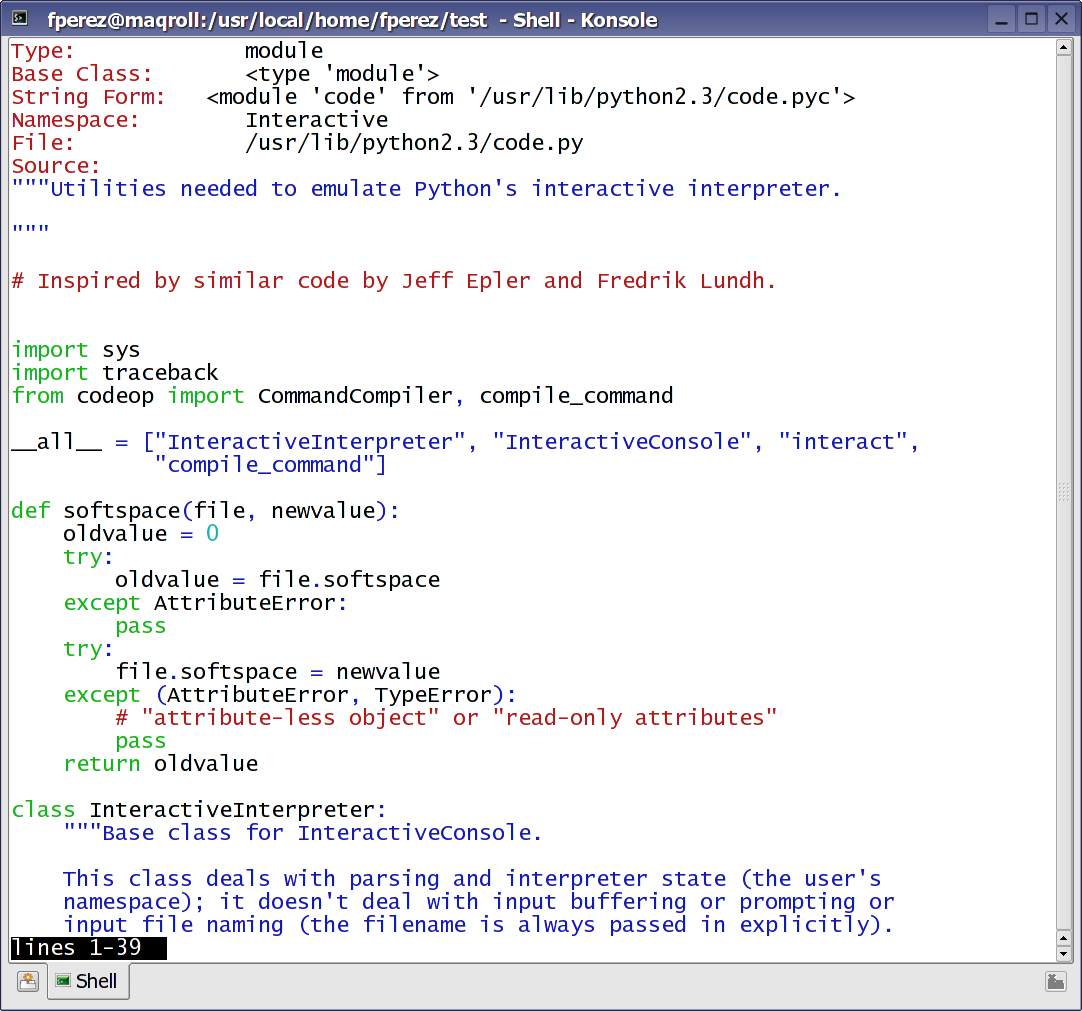
\includegraphics[width=0.48\linewidth]{fig/ipscr_code}~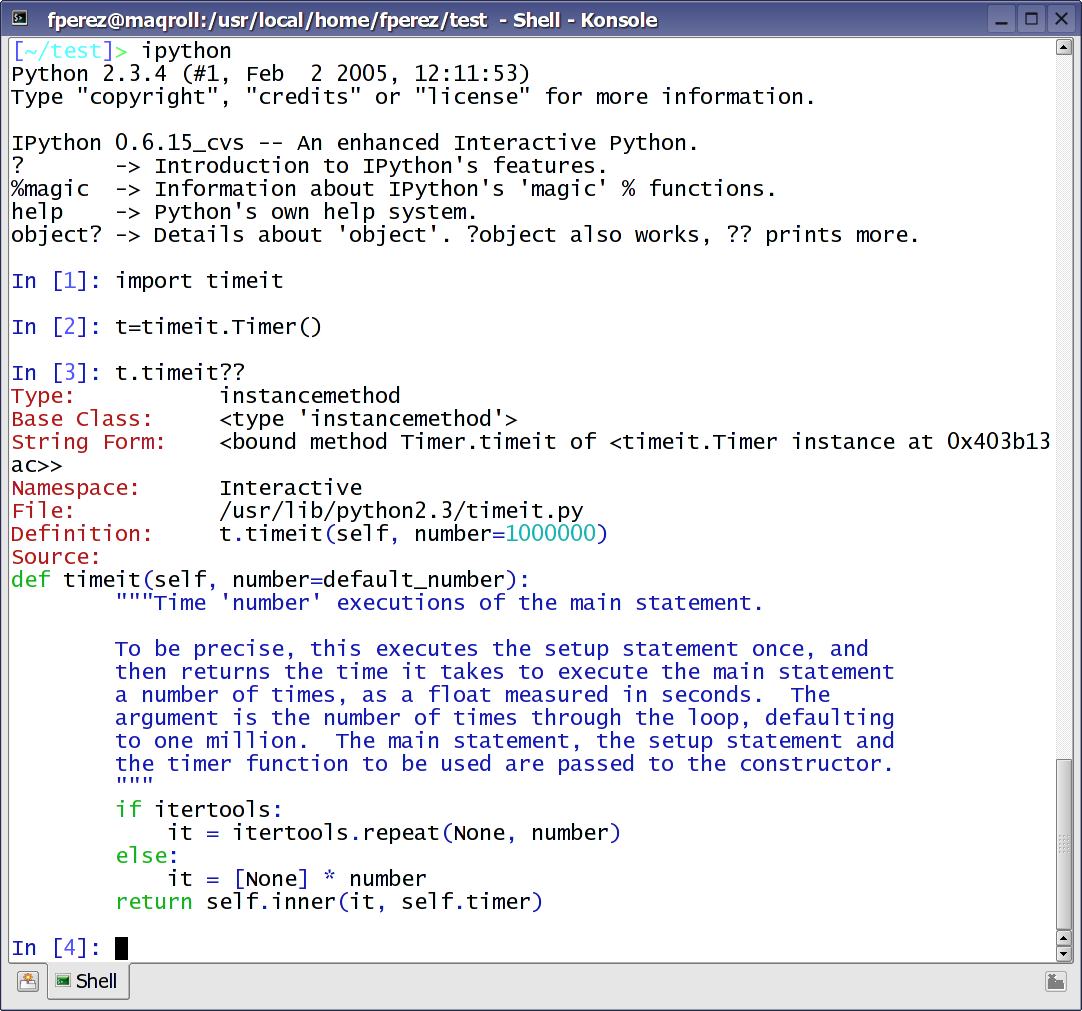
\includegraphics[width=0.48\linewidth]{fig/ipscr_meth_src}
\par\end{centering}

\caption{\label{fig:ipscr_code}IPython can show syntax-highlighted source
code for objects whose source is available.}

\end{figure}



\subsection{Input and Ouptut cached prompts}

In IPython, all output results are automatically stored in a global
dictionary named \texttt{Out} and variables named \texttt{\_1}, \texttt{\_2},
etc. alias them. For example, the result of input line 4 is available
either as \texttt{Out{[}4]} or as \texttt{\_4}. Additionally, three
variables named \texttt{\_}, \texttt{\_\_} and \texttt{\_\_\_} are
always kept updated with the for the last three results. This allows
you to recall any previous result and further use it for new calculations.
For example:

\begin{lyxcode}
In~{[}1]:~2+4

Out{[}1]:~6



In~{[}2]:~\_+9

Out{[}2]:~15



In~{[}3]:~\_+\_\_

Out{[}3]:~21



In~{[}4]:~print~\_1

6



In~{[}5]:~print~Out{[}1]

6



In~{[}6]:~\_2{*}{*}3

Out{[}6]:~3375
\end{lyxcode}
You can put a \texttt{`;}' at the end of a line to supress the printing
of output. This is useful when doing calculations which generate long
output you are not interested in seeing. The \texttt{\_{*}} variables
and the \texttt{Out{[}]} list do get updated with the contents of
the output, even if it is not printed. You can thus still access the
generated results this way for further processing.

A similar system exists for caching input. All input is stored in
a global list called \texttt{In} , so you can re-execute lines 22
through 28 plus line 34 by typing \texttt{'exec In{[}22:29]+In{[}34]'}
(using Python slicing notation). 

At any time, your input history remains available. The \texttt{\%hist}
command can show you all previous input, without line numbers if desired
(option \texttt{-n}) so you can directly copy and paste code either
back in IPython or in a text editor. You can also save all your history
by turning on logging via \texttt{\%logstart}; these logs can later
be either reloaded as IPython sessions or used as code for your programs.

If you need to execute the same set of lines often, you can assign
them to a macro with the \texttt{\%macro} magic function. Macros are
simply short names for groups of input lines, which can be re-executed
by only typing that name. Typing \texttt{macro?} at the prompt will
show you the function's full documentation. For example, if your history
contains:

\begin{lyxcode}
44:~x=1

45:~y=3

46:~z=x+y

47:~print~x

48:~a=5

49:~print~'x',x,'y',y
\end{lyxcode}
You can create a macro with lines 44 through 47 (included) and line
49 called \texttt{my\_macro} with:

\begin{lyxcode}
In~{[}51]:~\%macro~my\_macro~44:48~49
\end{lyxcode}
Now, simply typing \texttt{my\_macro} will re-execute all this code
in one pass. The number range follows standard Python list slicing
notation, where \texttt{n:m} means the numbers $(n,n+1,\ldots,m-1).$

You should note that macros execute in the current context, so if
any variable changes, the macro will pick up the new value every time
it is executed:

\begin{lyxcode}
In~{[}1]:~x=1

In~{[}2]:~y=x{*}5

In~{[}3]:~z=x+3

In~{[}4]:~print~'y~is:',y,'and~z~is:',z

y~is:~5~and~z~is:~4

\textcolor{blue}{\#~make~a~macro~with~lines~2,3,4~(note~Python~list~slice~syntax):}

In~{[}5]:~macro~yz~2:5

Macro~`yz`~created.~To~execute,~type~its~name~(without~quotes).

Macro~contents:

y=x{*}5

z=x+3

print~'y~is:',y,'and~z~is:',z

\textcolor{blue}{\#~now,~run~the~macro~directly:}

In~{[}6]:~yz

Out{[}6]:~Executing~Macro...

y~is:~5~and~z~is:~4

\textcolor{blue}{\#~we~change~the~value~of~x}

In~{[}7]:~x=9

\textcolor{blue}{\#~and~now~if~we~rerun~the~macro,~we~get~the~new~values:}

In~{[}8]:~yz

Out{[}8]:~Executing~Macro...

y~is:~45~and~z~is:~12
\end{lyxcode}

\subsection{Running code}

The \texttt{\%run} magic command allows you to run any python script
and load all of its data directly into the interactive namespace.
\texttt{\%run} is a sophisticated wrapper around the Python \texttt{execfile()}
builtin function; since the file is re-read from disk each time, changes
you make to it are reflected immediately (in contrast to the behavior
of \texttt{import}). I rarely use \texttt{import} for code I am testing,
relying on \texttt{\%run} instead. 

By default, 

\begin{lyxcode}
\%run~myfile~arg1~arg2~...
\end{lyxcode}
executes \texttt{myfile} in a namespace initially consisting only
of \texttt{\_\_name\_\_=='\_\_main\_\_'} and \texttt{sys.argv} being
filled with arg1, arg2, etc. This means that using \texttt{\%run}
is functionally very simlar to executing a script at the system command
line, but you get all the functionality of IPython (better tracebacks,
debugger and profiler access, etc.). The \texttt{-n} option prevents
\texttt{\_\_name\_\_} from being set equal to \texttt{'\_\_main\_\_'},
in case you want to test the part of a script which only runs when
\texttt{import}ed. 

Additionally, the fact that IPython then updates your interactive
namespace with the variables defined in the script is very useful,
because you can run your code to do a lot of processing, and then
continue using and exploring interactively the objects created by
the program. 

For example, if the file \texttt{ip\_simple.py} contains:

\lstinputlisting{examples/ip_simple.py}you can run it in IPython
as follows:

\begin{lyxcode}
\textcolor{blue}{\#~First,~let's~check~that~x~is~undefined}

In~{[}1]:~x

-{}-{}-{}-{}-{}-{}-{}-{}-{}-{}-{}-{}-{}-{}-{}-{}-{}-{}-{}-{}-{}-{}-{}-{}-{}-{}-{}-{}-{}-{}-{}-{}-{}-{}-{}-{}-{}-{}-{}-{}-{}-{}-{}-{}-{}-{}-{}-{}-{}-{}-{}-{}-{}-{}-{}-{}-{}-{}-{}-{}-{}-{}-{}-{}-{}-{}-{}-{}-{}-{}-{}-{}-{}-{}-

exceptions.NameError~~~~~~~~~~~~~~~~~~~~~~~~~~~~~~~~~Traceback~(most~recent~call~last)

/usr/local/home/fperez/teach/course/problems/<console>

NameError:~name~'x'~is~not~defined



\textcolor{blue}{\#~Now~we~run~the~script~(the~.py~extension~is~optional):}

In~{[}2]:~run~ip\_simple

sys.argv~is:~{[}'ip\_simple.py']

\_\_name\_\_~is:~\_\_main\_\_



\textcolor{blue}{\#~If~we~print~x,~now~it~has~the~value~from~the~script}

In~{[}3]:~x

Out{[}3]:~1



\textcolor{blue}{\#~Again,~but~now~running~with~some~arguments:}

In~{[}4]:~run~ip\_simple~-x~arg1~\char`\"{}hello~world\char`\"{}

sys.argv~is:~{[}'ip\_simple.py',~'-x',~'arg1',~'hello~world']

\_\_name\_\_~is:~\_\_main\_\_
\end{lyxcode}
With the \texttt{-i} option, the namespace where your script runs
is actually your interactive one. This can be used for two sligthly
different purposes. The simpler case, is just to quickly type up a
set of commands in an editor which you want to execute on your current
environment (although the \texttt{\%edit} command can also be used
for this). Consider running the file \texttt{ip\_simple2.py}:

\lstinputlisting{examples/ip_simple2.py}in IPython:

\begin{lyxcode}
\textcolor{blue}{\#~A~regular~\%run~will~produce~an~error:}

In~{[}1]:~run~ip\_simple2

-{}-{}-{}-{}-{}-{}-{}-{}-{}-{}-{}-{}-{}-{}-{}-{}-{}-{}-{}-{}-{}-{}-{}-{}-{}-{}-{}-{}-{}-{}-{}-{}-{}-{}-{}-{}-{}-{}-{}-{}-{}-{}-{}-{}-{}-{}-{}-{}-{}-{}-{}-{}-{}-{}-{}-{}-

exceptions.NameError~~~~~~~~~~~~~~Traceback~(most~recent~call~last)

/usr/local/home/fperez/teach/course/problems/ip\_simple2.py

~~~~~~2

~~~~~~3~It~should~be~run~via~IPython's~\%run~with~the~-i~option.\char`\"{}\char`\"{}\char`\"{}

~~~~~~4

-{}-{}-{}->~5~print~'x~is:',x

~~~~~~6

NameError:~name~'x'~is~not~defined

WARNING:~Failure~executing~file:~<ip\_simple2.py>

x~is:

\textcolor{blue}{\#~However,~if~you~do~have~a~variable~x~defined:}

In~{[}2]:~x='hello'

\textcolor{blue}{\#~you~can~use~the~-i~option~and~the~code~will~see~x:}

In~{[}3]:~run~-i~ip\_simple2

x~is:~hello
\end{lyxcode}
A different use of \texttt{\%run -i}, is to repeatedly run scripts
which may have a potentially expensive initialization phase. If this
initialization does not need to be repeated on each run (for example,
you are debugging some other submodule and can reuse the same expensive
object several times), you can avoid it by protecting the expensive
object with a \texttt{try/except} block. This simple script illustrates
the technique:

\lstinputlisting{examples/ip_expensive_init.py}In IPython, here is
how you can use it:

\begin{lyxcode}
\textcolor{blue}{\#~The~first~time~it~runs,~it~will~have~to~initialize}

In~{[}1]:~run~-i~ip\_expensive\_init.py

bigobject~not~found,~performing~expensive~initialization...

total~is:~499500

\textcolor{blue}{\#~but~successive~runs~don't~require~initialization}

In~{[}2]:~run~-i~ip\_expensive\_init.py

We~found~bigobject!~No~need~to~initialize~it.

total~is:~499500

\textcolor{blue}{\#~you~can~still~run~without~-i,~to~achieve~a~full~reload~}

\textcolor{blue}{\#~if~you~need~it~for~any~reason}

In~{[}3]:~run~ip\_expensive\_init.py

bigobject~not~found,~performing~expensive~initialization...

total~is:~499500
\end{lyxcode}
In the third run, by not using \texttt{-i}, your script runs in an
empty namespace and this forces a full initialization (the \texttt{NameError}
exception is triggered).

\texttt{\%run} also has special flags for timing the execution of
your scripts (\texttt{-t}) and for executing them under the control
of either Python's \texttt{pdb} debugger (\texttt{-d}) or profiler
(\texttt{-p}). You can get all of its docstring with the usual \texttt{run?}
mechanism.

Thanks to all of its various control options, \texttt{\%run} can be
used as the main tool for efficient interactive development of code
which you write in your editor of choice. My personal operation mode,
which has served me well for several years of scientific work in Python,
is to have a good editor (XEmacs in my case) open with all my Python
code, and IPython open in a terminal where I run, debug, explore,
plot, etc.


\section[OS access]{Access to the underlying Operating System}


\subsection{Basic usage}

IPython allows you to always access the underlying OS very easily.
Any lines starting with \texttt{!} are passed directly to the system
shell:

\begin{lyxcode}
In~{[}6]:~!ls~ip{*}.py

ip\_expensive\_init.py~~ip\_simple2.py~~ip\_simple.py
\end{lyxcode}
and using \texttt{!!} captures shell output into python variables
for further use:

\begin{lyxcode}
In~{[}7]:~!!ls~ip{*}.py

Out{[}7]:~{[}'ip\_expensive\_init.py',~'ip\_simple2.py',~'ip\_simple.py']
\end{lyxcode}
There is a difference between the two cases: in the first, the \texttt{ls}
command simply prints its results to the terminal as text, but no
value is returned. In the second, IPython actually captures the output
of the command, splits it as a list (one line per entry), and returns
its value. This allows you to then operate on the results with Python
routines.

Additionally, IPython plays a few interesting syntactic tricks for
your convenience. Whenever you make a system call, IPython will expand
any call of the type \texttt{\$var} into the actual value of the python
variable \texttt{var}, so that you can call shell commands on Python
values. Continuing the session above, and remembering that \texttt{\_}
holds the previously returned value, we can call the `\texttt{wc -l}'
Unix command (which does a line count on a file) on the files we just
obtained:

\begin{lyxcode}
In~{[}8]:~for~f~in~\_:

~~~...:~~~~~~if~'simple'~in~f:

~~~...:~~~~~~~~~~!wc~-l~\$f

~~~...:

3~ip\_simple2.py

4~ip\_simple.py
\end{lyxcode}
While this is completely unorthodox (actually, invalid) Python, it
is the kind of functionality which can make for extremely efficient
uses when working at an interactive command line. Obviously all of
this can be done (and it \emph{is} done that way by IPython internally)
with regular Python code, but that approach requires a fair amount
more typing, the use of \texttt{\%}-based string interpolation, and
making system calls via the \texttt{os.system()} function.

If you actually need to pass a \texttt{\$} character to a shell command,
you simply use \texttt{\$\$} in the IPython command line:

\begin{lyxcode}
In~{[}11]:~!echo~\$\$SHELL

/bin/tcsh
\end{lyxcode}
If you want to capture the output of a system command directly to
a named Python variable, you can use the \texttt{\%sc} magic function:

\begin{lyxcode}
\textcolor{blue}{\#~by~default,~\%sc~captures~to~a~plain~string:}

In~{[}16]:~\%sc~astr=ls~ip{*}.py

In~{[}17]:~astr

Out{[}17]:~'ip\_expensive\_init.py\textbackslash{}nip\_simple2.py\textbackslash{}nip\_simple.py'

\textcolor{blue}{\#~but~with~the~-l~option,~it~splits~to~a~list~(like~!!~does)}

In~{[}18]:~\%sc~-l~alist=ls~ip{*}.py

In~{[}19]:~alist

Out{[}19]:~{[}'ip\_expensive\_init.py',~'ip\_simple2.py',~'ip\_simple.py']
\end{lyxcode}

\subsection{System aliases}

In IPython, you can also define your own system aliases. Even though
IPython gives you access to your system shell via the \texttt{!} prefix,
it is convenient to have aliases to the system commands you use most
often. This allows you to work seamlessly from inside IPython with
the same commands you are used to in your system shell:

\texttt{`\%alias alias\_name cmd'} defines \texttt{`alias\_name'}
as an alias for \texttt{`cmd'}

Then, typing \texttt{`alias\_name params'} will execute the system
command \texttt{`cmd params'} (from your underlying operating system).
Aliases have lower precedence than magic functions and Python normal
variables, so if \texttt{`foo'} is both a Python variable and an alias,
the alias can not be executed until \texttt{`del foo'} removes the
Python variable. If you need to access an alias directly, you can
use the builtin function \texttt{ipalias} as \texttt{ipalias('foo')}.

You can use the \texttt{\%l} specifier in an alias definition to represent
the whole line when the alias is called. For example:

\begin{lyxcode}
In~{[}2]:~alias~all~echo~\char`\"{}Input~in~brackets:~<\%l>\char`\"{}

In~{[}3]:~all~hello~world

Input~in~brackets:~<hello~world>
\end{lyxcode}
You can also define aliases with positional parameters using \texttt{\%s}
specifiers (one per parameter):

\begin{lyxcode}
In~{[}1]:~alias~parts~echo~first~\%s~second~\%s

In~{[}2]:~\%parts~A~B

first~A~second~B

In~{[}3]:~\%parts~A

Incorrect~number~of~arguments:~2~expected.

parts~is~an~alias~to:~'echo~first~\%s~second~\%s'
\end{lyxcode}
Aliases expand Python variables just like system calls using \texttt{!}
or \texttt{!!} do: all expressions prefixed with '\texttt{\$}' get
expanded. For details of the semantic rules, see PEP-215: \url{http://www.python.org/peps/pep-0215.html}.
This is the library used by IPython for variable expansion.

Simply typing \texttt{alias} will print a list of the current aliases,
and \texttt{unalias} can be used to remove an alias. For further details,
use \texttt{alias?}.


\subsection{Directory management}

IPython comes with some pre-defined aliases and a complete system
for changing directories, both via a stack (see \texttt{\%pushd},
\texttt{\%popd} and \texttt{\%ds}) and via direct \texttt{\%cd}. The
latter keeps a history of visited directories and allows you to go
to any previously visited one. You can see this history with the \texttt{\%dhist}
magic:

\begin{lyxcode}
In~{[}1]:~cd~\textasciitilde{}/code/python

/home/fperez/code/python

In~{[}2]:~cd~\textasciitilde{}/teach/

/home/fperez/teach

In~{[}3]:~cd~\textasciitilde{}/research

/home/fperez/research

In~{[}4]:~dhist

Directory~history~(kept~in~\_dh)

0:~/home/fperez/teach/course/examples

1:~/home/fperez/code/python

2:~/home/fperez/teach

3:~/home/fperez/research

In~{[}5]:~cd~-1

/home/fperez/code/python
\end{lyxcode}
The \texttt{\%bookmark} magic allows you to create named bookmarks
in your filesystem, which \texttt{cd} can be directed to go to (with
the \texttt{-b} flag), and to which it will try to default automatically
if no such named directory exists. The system is very easy to use
and quite natural in practice:

\begin{lyxcode}
In~{[}8]:~bookmark~course

In~{[}9]:~cd

/home/fperez

In~{[}10]:~ls~course

ls:~course:~No~such~file~or~directory

In~{[}11]:~cd~course

(bookmark:course)~->~/home/fperez/teach/course

/home/fperez/teach/course
\end{lyxcode}

\subsection{IPython as a system shell}

While IPython is \emph{not} a system shell, it ships with a special
profile called \texttt{pysh}, which you can activate at the command
line as \texttt{`ipython -p pysh'}. This modifies IPython's behavior
and adds some additional facilities and a prompt customized for filesystem
navigation.

Note that this does \emph{not} make IPython a full-fledged system
shell. In particular, it has no job control, so if you type Ctrl-Z
(under Unix), you'll suspend pysh itself, not the process you just
started. 

What the shell profile allows you to do is to use the convenient and
powerful syntax of Python to do quick scripting at the command line.
Below we describe some of its features.


\subsubsection{Aliases}

All of your \texttt{\$PATH} has been loaded as IPython aliases, so
you should be able to type any normal system command and have it executed.
See \texttt{\%alias?} and \texttt{\%unalias?} for details on the alias
facilities. See also \texttt{\%rehash?} and \texttt{\%rehashx?} for
details on the mechanism used to load \texttt{\$PATH}.


\subsubsection{Special syntax}

Any lines which begin with \texttt{`\textasciitilde{}'}, \texttt{`/'}
and \texttt{`.'} will be executed as shell commands instead of as
Python code. The special escapes below are also recognized. \texttt{!cmd}
is valid in single or multi-line input, all others are only valid
in single-line input:

\begin{description}
\item [{\texttt{!cmd}}] pass `cmd' directly to the shell 
\item [{\texttt{!!cmd}}] execute `cmd' and return output as a list (split
on `\textbackslash{}n') 
\item [{\texttt{\$var=cmd}}] capture output of cmd into var, as a string
(shorthand for \texttt{\%sc var=cmd})
\item [{\texttt{\$\$var=cmd}}] capture output of cmd into var, as a list
(split on `\textbackslash{}n', shorthand for \texttt{\%sc -l var=cmd})
\end{description}

\subsubsection{Useful functions and modules}

The os, sys and shutil modules from the Python standard library are
automatically loaded. Some additional functions, useful for shell
usage, are listed below. You can request more help about them with
`\texttt{?}'.

\begin{description}
\item [{\texttt{shell}}] - execute a command in the underlying system shell 
\item [{\texttt{system}}] - like \texttt{shell()}, but return the exit
status of the command
\item [{\texttt{sout}}] - capture the output of a command as a string
\item [{\texttt{lout}}] - capture the output of a command as a list (split
on `\textbackslash{}n')
\item [{\texttt{getoutputerror}}] - capture (output,error) of a shell commandss
\end{description}
\texttt{sout}/\texttt{lout} are the functional equivalents of \texttt{\$}/\texttt{\$\$}.
They are provided to allow you to capture system output in the middle
of true python code, function definitions, etc (where \texttt{\$}
and \texttt{\$\$} are invalid)


\section{Access to an editor}

You can use \texttt{\%edit} to have almost multiline editing. While
IPython doesn't support true multiline editing, this command allows
you to call an editor on the spot, and IPython will execute the code
you type in there as if it were typed interactively. 

\texttt{\%edit} runs your IPython configured editor. By default this
is read from your environment variable \texttt{\$EDITOR}. If this
isn't found, it will default to \texttt{vi} under Linux/Unix and to
\texttt{notepad} under Windows. 

You can also set the value of this editor via the command-line option
\texttt{`-editor'} or in your \texttt{ipythonrc} file. This is useful
if you wish to use specifically for IPython an editor different from
your typical default (and for Windows users who typically don't set
environment variables).

This command allows you to conveniently edit multi-line code right
in your IPython session.

If called without arguments, \texttt{\%edit} opens up an empty editor
with a temporary file and will execute the contents of this file when
you close it (don't forget to save it!). 


\section{Customizing IPython}


\subsection{Basics}

IPython has a very flexible configuration system. It uses a configuration
file which allows permanent setting of all command-line options, module
loading, code and file execution. The system allows recursive file
inclusion, so you can have a base file with defaults and layers which
load other customizations for particular projects.

IPython reads a configuration file which can be specified at the command
line (\texttt{-rcfile}) or which by default is assumed to be called
\texttt{ipythonrc}. Such a file is looked for in the current directory
where IPython is started and then in your \texttt{IPYTHONDIR}, which
allows you to have local configuration files for specific projects.
The default value for this directory is \texttt{\$HOME/.ipython} (\texttt{\_ipython}
under Windows). Under Unix operating systems \texttt{\$HOME} always
exists; for Windows, IPython will try to find such an environment
variable; if it doesn't exist, it uses \texttt{HOMEDRIVE\textbackslash{}HOMEPATH}
(these are always defined by Windows). This typically gives something
like \texttt{C:\textbackslash{}Documents and Settings\textbackslash{}YourUserName},
but your local details may vary. Finally, you can make this directory
live anywhere you want by creating an environment variable called
\texttt{\$IPYTHONDIR}.

In this directory you will find all the files that configure IPython's
defaults, and you can put there your profiles and extensions. This
directory is automatically added by IPython to \texttt{sys.path},
so anything you place there can be found by \texttt{import} statements.

The syntax of an rcfile is one of key-value pairs separated by whitespace,
one per line. Lines beginning with a \texttt{\#} are ignored as comments,
but comments can \textbf{not} be put on lines with data (the parser
is fairly primitive). You can study the default rcfile created by
IPython at startup for customization details, it is extremely commented.


\subsection{Profiles}

IPython can load any configuration file you want if you give its name
at startup with the \texttt{-rcfile} flag. However, for convenience
it provides a shorthand based on a naming convention for loading such
profiles. This system allows you to easily maintain customized versions
of IPython for specific purposes.

With the \texttt{-profile <name>} flag (you can abbreviate it to \texttt{-p}),
IPython will assume that your config file is called \texttt{ipythonrc-<name>}
(it looks in current dir first, then in \texttt{IPYTHONDIR}). This
is a quick way to keep and load multiple config files for different
tasks, especially if you use the include option of config files. You
can keep a basic \texttt{IPYTHONDIR/ipythonrc} file and then have
other profiles which include this one and load extra things for particular
tasks. For example:

\begin{enumerate}
\item \texttt{\$HOME/.ipython/ipythonrc}: load basic things you always want. 
\item \texttt{\$HOME/.ipython/ipythonrc-math}: load (1) and basic math-related
modules. 
\item \texttt{\$HOME/.ipython/ipythonrc-numeric}: load (1) and Numeric and
plotting modules.
\end{enumerate}
Since it is possible to create an endless loop by having circular
file inclusions, IPython will stop if it reaches 15 recursive inclusions.


\section[Debugging and profiling]{Debugging and profiling with IPython }

The Python standard library includes powerful facilities for debugging
and profiling code, but it is common to find even experienced Python
programmers who still do not take advantage of them. In part, this
is due to the fact that loading and configuring them requires reading
an extra documentation section, and keeping a bit of additional information
about their use in your head. IPython tries to automate their use
to the point where, with a single command, you can use either of these
subsystems in a transparent manner. Hopefully they will become part
of your daily workflow.

At its most basic, for debugging your programs, you can rely on using
\texttt{\%run} to execute them, see the results, play with all variables
loaded into the interactive namespace, etc. A typical working session
involves keeping your favorite editor open with the file you are working
on, and repeatedly calling \texttt{\%run} on it as you make changes
and save them.

%
\begin{figure}
\begin{centering}
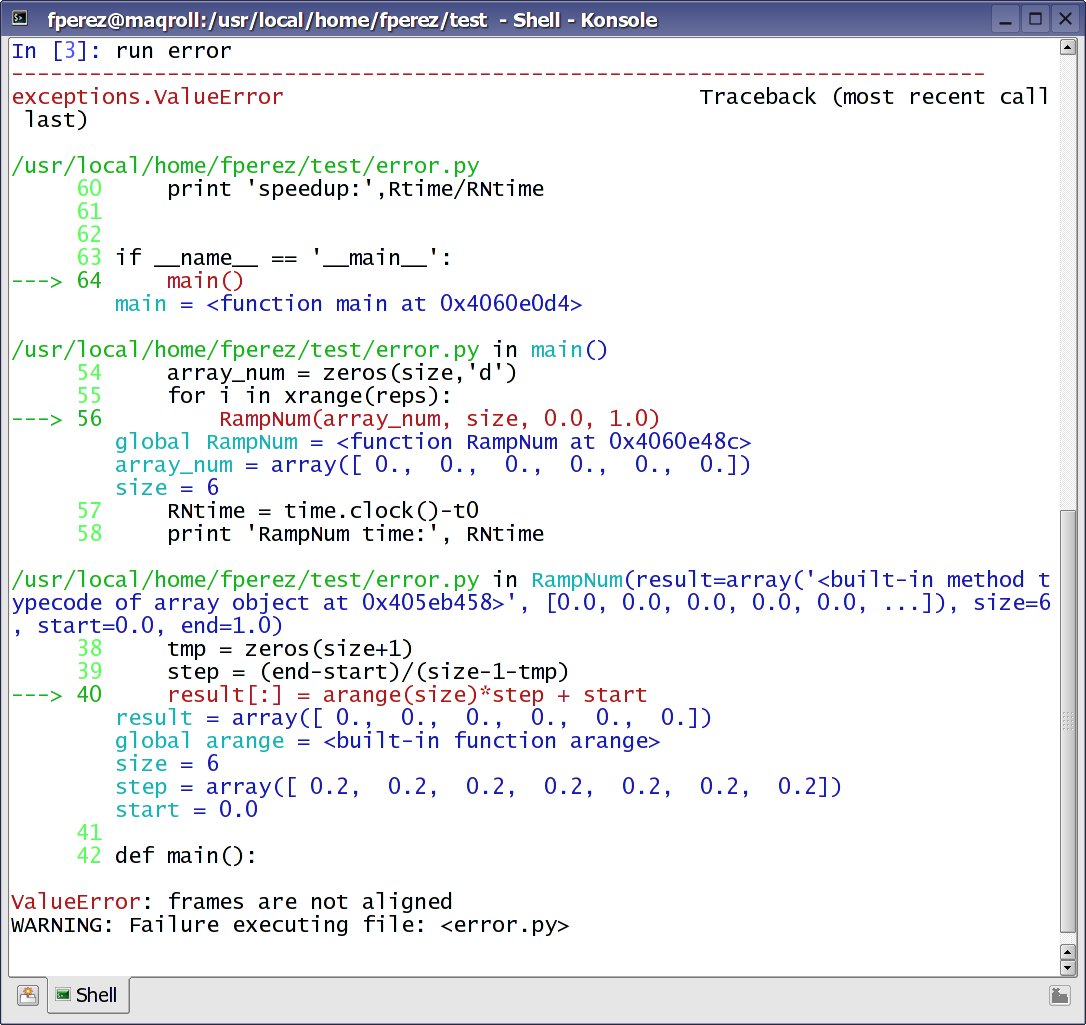
\includegraphics[width=0.7\linewidth]{fig/ipscr_traceback}
\par\end{centering}

\caption{\label{fig:ipscr_traceback}IPython can provide extremely detailed
tracebacks.}

\end{figure}


If your program raises an exception, IPython will provide you with
a more detailed traceback than the default Python ones. You can even
increase the level of detail further by using \texttt{\%xmode Verbose},
which forces the printing of variable values at all stack frames.
This option should be used with care though (and that's why it is
not the default), as printing a ten-million-entry array can lock up
your computer for a very long time. An example of this kind of very
informative traceback is shown in Fig.~\ref{fig:ipscr_traceback}.


\subsection{Automatic invocation of \texttt{pdb} on exceptions}

IPython, if started with the \texttt{-pdb} option (or if the option
is set in your rc file) can call the Python \texttt{pdb} debugger
every time your code triggers an uncaught exception. This feature
can also be toggled at any time with the \texttt{\%pdb} magic command.
This can be extremely useful in order to find the origin of subtle
bugs, because \texttt{pdb} opens up at the point in your code which
triggered the exception, and while your program is at this point `dead',
all the data is still available and you can walk up and down the stack
frame and understand the origin of the problem.

Furthermore, you can use these debugging facilities both with the
embedded IPython mode and without IPython at all. For an embedded
shell (see sec. \ref{sec:ipython_embed}), simply call the constructor
with \texttt{`-pdb'} in the argument string and automatically \texttt{pdb}
will be called if an uncaught exception is triggered by your code. 

For stand-alone use of the feature in your programs which do not use
IPython at all, put the following lines toward the top of your `main'
routine:

\begin{lyxcode}
import~sys,IPython.ultraTB

sys.excepthook~=~IPython.ultraTB.FormattedTB(mode=`Verbose',~~\\
color\_scheme=`Linux',~call\_pdb=1)
\end{lyxcode}
The \texttt{mode} keyword can be either \texttt{`Verbose'} or \texttt{`Plain'},
giving either very detailed or normal tracebacks respectively. The
\texttt{color\_scheme} keyword can be one of \texttt{`NoColor'}, \texttt{`Linux'}
(default) or \texttt{`LightBG'}. These are the same options which
can be set in IPython with \texttt{-colors} and \texttt{-xmode}.

This will give any of your programs detailed, colored tracebacks with
automatic invocation of \texttt{pdb}.


\subsection{Running entire programs via \texttt{pdb}}

\texttt{pdb}, the Python debugger, is a powerful interactive debugger
which allows you to step through code, set breakpoints, watch variables,
etc. IPython makes it very easy to start any script under the control
of \texttt{pdb}, regardless of whether you have wrapped it into a
\texttt{`main()'} function or not. For this, simply type \texttt{`\%run
-d myscript'} at an IPython prompt. See the \texttt{\%run} command's
documentation (\texttt{run?}) for more details, including how to control
where \texttt{pdb} will stop execution first.

For more information on the use of the \texttt{pdb} debugger, read
the included \texttt{pdb.doc} file (part of the standard Python distribution).
On a stock Linux system it is located at \texttt{/usr/lib/python2.3/pdb.doc},
but the easiest way to read it is by using the \texttt{help()} function
of the \texttt{pdb} module as follows (in an IPython prompt):

\begin{lyxcode}
In~{[}1]:~import~pdb

In~{[}2]:~pdb.help()
\end{lyxcode}
This will load the \texttt{pdb.doc} document in a file viewer for
you automatically.


\subsection{Profiling}

When dealing with performance issues, the \texttt{\%run} command with
a \texttt{-p} option allows you to run complete programs under the
control of the Python profiler. The \texttt{\%prun} command does a
similar job for single Python expressions (like function calls, similar
to \texttt{profile.run()}). While this is possible with the standard
\texttt{profile} module, IPython wraps this functionality with magic
commands convenient for rapid interactive work.


\section[Embedding]{\label{sec:ipython_embed}Embedding IPython into your programs }

A few lines of code are enough to load a complete IPython inside your
own programs, giving you the ability to work with your data interactively
after automatic processing has been completed. 

You can call IPython as a python shell inside your own python programs.
This can be used both for debugging code or for providing interactive
abilities to your programs with knowledge about the local namespaces
(very useful in debugging and data analysis situations).

It is possible to start an IPython instance \emph{inside} your own
Python programs. This allows you to evaluate dynamically the state
of your code, operate with your variables, analyze them, etc. Note
however that any changes you make to values while in the shell do
\emph{not} propagate back to the running code, so it is safe to modify
your values because you won't break your code in bizarre ways by doing
so.

This feature allows you to easily have a fully functional python environment
for doing object introspection anywhere in your code with a simple
function call. In some cases a simple print statement is enough, but
if you need to do more detailed analysis of a code fragment this feature
can be very valuable.

It can also be useful in scientific computing situations where it
is common to need to do some automatic, computationally intensive
part and then stop to look at data, plots, etc%
\footnote{This functionality was inspired by IDL's combination of the \texttt{stop}
keyword and the \texttt{.continue} executive command, which I have
found very useful in the past, and by a posting on comp.lang.python
by cmkl <cmkleffner@gmx.de> on Dec. 06/01 concerning similar uses
of pyrepl.%
}. Opening an IPython instance will give you full access to your data
and functions, and you can resume program execution once you are done
with the interactive part (perhaps to stop again later, as many times
as needed).

The following code snippet is the bare minimum you need to include
in your Python programs for this to work (detailed examples follow
later):

\begin{lyxcode}
from~IPython.Shell~import~IPShellEmbed

ipshell~=~IPShellEmbed()

ipshell()~\#~this~call~anywhere~in~your~program~will~start~IPython
\end{lyxcode}
You can run embedded instances even in code which is itself being
run at the IPython interactive prompt with '\texttt{\%run~<filename>}'.
Since it's easy to get lost as to where you are (in your top-level
IPython or in your embedded one), it's a good idea in such cases to
set the in/out prompts to something different for the embedded instances.
The code examples below illustrate this.

You can also have multiple IPython instances in your program and open
them separately, for example with different options for data presentation.
If you close and open the same instance multiple times, its prompt
counters simply continue from each execution to the next.

Please look at the docstrings in the \texttt{Shell.py} module for
more details on the use of this system.

The following sample file illustrating how to use the embedding functionality
is provided in the examples directory as \texttt{example-embed.py}.
It should be fairly self-explanatory:

\lstinputlisting{examples/ip_embed.py}

Once you understand how the system functions, you can use the following
code fragments in your programs which are ready for cut and paste:

\lstinputlisting{examples/ip_embed-short.py}


\section[Matplotlib]{\label{sec:ipython_pylab}Integration with Matplotlib}

The matplotlib library (\url{http://matplotlib.sourceforge.net})
provides high quality 2D plotting for Python. Matplotlib can produce
plots on screen using a variety of GUI toolkits, including Tk, GTK
and WXPython. It also provides a number of commands useful for scientific
computing, all with a syntax compatible with that of the popular Matlab
program.

IPython accepts the special option \texttt{-pylab}. This configures
it to support matplotlib, honoring the settings in the \texttt{.matplotlibrc}
file. IPython will detect the user's choice of matplotlib GUI backend,
and automatically select the proper threading model to prevent blocking.
It also sets matplotlib in interactive mode and modifies \texttt{\%run}
slightly, so that any matplotlib-based script can be executed using
\texttt{\%run} and the final \texttt{show()} command does not block
the interactive shell.

The \texttt{-pylab} option must be given first in order for IPython
to configure its threading mode. However, you can still issue other
options afterwards. This allows you to have a matplotlib-based environment
customized with additional modules using the standard IPython profile
mechanism: ``\texttt{ipython -pylab -p myprofile}'' will load the
profile defined in \texttt{ipythonrc-myprofile} after configuring
matplotlib.



\chapter[matplotlib]{Introduction to plotting with matplotlib / pylab}


\section[Overview]{A bird's eye view}

matplotlib is a library for making 2D plots of arrays in python.%
\footnote{This short guide is not meant as a complete guide or tutorial. There
  is a more comprehensive user's guide and tutorial on the matplotlib web-site
  at http://matplotlib.sf.net.%
} Although it has its origins in emulating the Matlab graphics commands, it
does not require matlab, and has a pure, object oriented API. Although
matplotlib is written primarily in python, it makes heavy use of NumPy and
other extension code to provide good performance even for large
arrays. matplotlib is designed with the philosophy that you should be able to
create simple plots with just a few commands, or just one!  If you want to see
a histogram of your data, you shouldn't need to instantiate objects, call
methods, set properties, and so on; it should just work.

The matplotlib code is divided into three parts: the \textit{pylab
interface} is the set of functions provided by the \texttt{pylab}
module which allow the user to create plots with code quite similar
to matlab figure generating code. The matplotlib frontend or \textit{matplotlib
API} is the set of classes that do the heavy lifting, creating and
managing figures, text, lines, plots and so on. This is an abstract
interface that knowns nothing about output formats. The \textit{backends}
are device dependent drawing devices, aka renderers, that transform
the frontend representation to hardcopy or a display device. Example
backends: PS creates postscript hardcopy, SVG creates scalar vector
graphics hardcopy, Agg creates PNG output using the high quality antigrain
library that ships with matplotlib, GTK embeds matplotlib in a GTK
application, GTKAgg uses the antigrain%
\footnote{http://antigrain.com%
} renderer to create a figure and embed it a GTK application, and so
on for WX, Tkinter, FLTK, \ldots{}.

For years, I used to use matlab exclusively for data analysis and
visualization. matlab excels at making nice looking plots easy. When
I began working with EEG data, I found that I needed to write applications
to interact with my data, and developed and EEG analysis application
in matlab. As the application grew in complexity, interacting with
databases, http servers, manipulating complex data structures, I began
to strain against the limitations of matlab as a programming language,
and decided to start over in python. python more than makes up for
all of matlab's deficiencies as a programming language, but I was
having difficulty finding a 2D plotting package -- for 3D VTK, which
is discussed at length below more than exceeds all of my needs.

When I went searching for a python plotting package, I had several
requirements: 

\begin{itemize}
\item Plots should look great - publication quality. One important requirement
for me is that the text looks good (antialiased, etc)
\item Postscript output for inclusion with \LaTeX{} documents and publication
quality printing
\item Embeddable in a graphical user interface for application development
\item The code should be mostly python so itis easy to understand and extend
-- users become developers!
\item Making plots should be easy -- just a few lines of code for simple
graphs
\end{itemize}
Finding no package that suited me just right, I did what any self-respecting
python programmer would do: rolled up my sleeves and dived in. Not
having any real experience with computer graphics, I decided to emulate
matlab's plotting capabilities because that is something matlab does
very well. This had the added advantage that many people have a lot
of matlab experience, and thus they can quickly get up to steam plotting
in python. From a developer's perspective, having a fixed user interface
(the pylab interface) has been very useful, because the guts of the
code base can be redesigned without affecting user code. 

Without further ado, let's create our first figure. This example uses
the matplotlib object oriented API. Most users use the pylab interface,
which will be discussed next and makes it easier to make plots because
a lot of the tedius work of creating and managing figures and figure
windows is done for you behind the hood. But since the real core of
the library is the object oriented API, I think it is a good place
to start. If you are developing a graphical user interface or making
plots on a web server, you probably want maximal control with no magic
going on behind the scenes -- this is where the matplotlib API should
be used. If you are just trying to make a figure for inclusion in
a paper or if your working interactively from the python shell, you'll
probably be happy with the pylab interface.

\lstinputlisting[caption={Creating a simple figure with the antigrain backend (generates PNG) using the object oriented matplotlib library}]{examples/mpl_agg_oo.py}

%
\begin{figure}
\begin{centering}
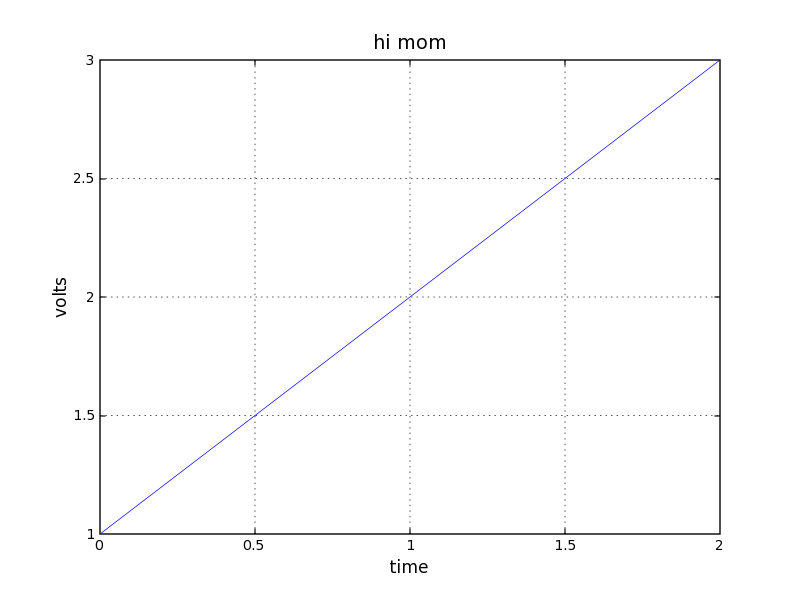
\includegraphics[width=4in]{fig/mpl_one_two_three}
\par\end{centering}

\caption{\label{fig:mpl_agg}A simple plot generated by the antigrain (Agg)
backend .}

\end{figure}



\section[pylab tutorial]{A short pylab tutorial}

Here is about the simplest code you can use to create a figure with
matplotlib using the pylab interface. In this section, I'm assuming
you are using ipython in the pylab mode -- see Section\ref{sec:ipython_pylab}
for details.

\begin{lyxcode}
peds-pc311:\textasciitilde{}>~pylab

Python~2.3.3~(\#2,~Apr~13~2004,~17:41:29)

Type~\char`\"{}copyright\char`\"{},~\char`\"{}credits\char`\"{}~or~\char`\"{}license\char`\"{}~for~more~information.

~

IPython~0.6.12\_cvs~-{}-~An~enhanced~Interactive~Python.

?~~~~~~~->~Introduction~to~IPython's~features.

\%magic~~->~Information~about~IPython's~'magic'~\%~functions.

help~~~~->~Python's~own~help~system.

object?~->~Details~about~'object'.~?object~also~works,~??~prints~more.

~

~~Welcome~to~pylab,~a~matplotlib-based~Python~environment

~~~~help(matplotlib)~->~generic~matplotlib~information

~~~~help(pylab)~~~~~~->~matlab-compatible~commands~from~matplotlib

~~~~help(plotting)~~~->~plotting~commands

~

In~{[}1]:~plot({[}1,2,3])

Out{[}1]:~{[}<matplotlib.lines.Line2D~instance~at~0xb557a86c>]
\end{lyxcode}
%
\begin{figure}
\begin{centering}

\includegraphics[width=5in]{fig/mpl_toolbar}
\par\end{centering}

\caption{\label{fig:mpl_toolbar}The matplotlib toolbar used to navigate around
your figure}

\end{figure}


If your settings are correct, a figure window should popup and you
should be able to interact with it. That's a lot less typing than
our initial example using the object oriented API in which you had
to manually create the Figure, Axes and so on!

Try clicking on the navigation toolbar at the bottom of the figure
-- the toolbar is shown in Figure\ref{fig:mpl_toolbar}. The first
three buttons from left to right in Figure\ref{fig:mpl_toolbar} are
\textit{home}, \textit{back} and \textit{forward}. These byttons are
are akin to the web browser buttons. They are used to navigate back
and forth between previously defined views. They have no meaning unless
you have already navigated somewhere else using the pan and zoom buttons
as described below. This is analogous to trying to click \texttt{Back}
on your web browser before visiting a new page --nothing happens.
The home button always takes you to the first, default view of your
data. 

The next to button moving right is the pan/zoom button, which looks
like a cross with arrows on the end (a \textit{fleur}). The pan/zoom
button button has two modes: pan and zoom (no surprise there, right?).
Click this toolbar button to activate this mode; you should see {}``pan/zoom
mode'' show up in the status bar. Then put your mouse somewhere over
an axes. To activate panning: press the left mouse button and hold
it, dragging it to a new position. If you press \texttt{x} or \texttt{y}
while panning, the motion will be contrained to the x or y axis, respectively
. To activate zooming, press the right mouse button, dragging it to
a new position. The x axis will be zoomed in proportionate to the
rightward movement and zoomed out proportionate to the leftward movement.
Ditto for the yaxis and up/down motions. The point under your mouse
when you begin the zoom remains stationary, allowing you to zoom to
an arbitrary point in the figure. You can use the modifier keys \texttt{x},
\texttt{y} or \texttt{CONTROL} to constrain the zoom to the x axes,
the y axes, or aspect ratio preserve, respectively.

The next button moving right is the \textit{zoom to rectangle button}
which has a magnifying glass over a piece of paper. The button is
striaghtforward and works in the standard way; when you click it,
you should see that it is activated by looking for {}``Zoom to rect
mode'' in the status bar, and then you select the rectangular region
you want to zoom in on.

The final button is the \textit{save button}, which will save your
figure in the current view. All of the {*}Agg backends know how to
save the following image types: PNG, PS, EPS, SVG. 

Let's make the same figure we made using the object oriented API above,
ie Figure\ref{fig:mpl_agg}, but this time using the pylab\lstinputlisting[caption={Creating a simple figure in pylab}]{examples/mpl_pylab.py}

As you can see there is basically a direct translation between the
OO interface and the pylab interface. When \texttt{plot} is called,
the pylab interface makes a call to the function \texttt{gca()} (``get
current axes'') to get a reference to the current axes. \texttt{gca}
in turn, makes a call to \texttt{gcf} ({}``get current figure'')
to get a reference to the current figure. \texttt{gcf}, finding that
no figure has been created, creates the default figure using \texttt{figure()}
and returns it. \texttt{gca} will then return the current axes of
that figure if it exists, or create the default axes \texttt{subplot(111)}
if it does not. The last line show is a GUI independent way of actually
creating a figure window, and is not required for image backends such
as postscript.

Thus a lot happens under the hood when you call plot, but for the
most part you don't need to think about it -- it just works. The important
thing to understand is that the pylab interface has a state, and keeps
track of the current figure and axes. All plotting commands target
the current axes, and you can manipulate which ones are current

\lstinputlisting[caption={Creating multiple subplots and plotting multiple lines in a single plot command}]{examples/mpl_subplot_demo.py}

%
\begin{figure}
\begin{centering}
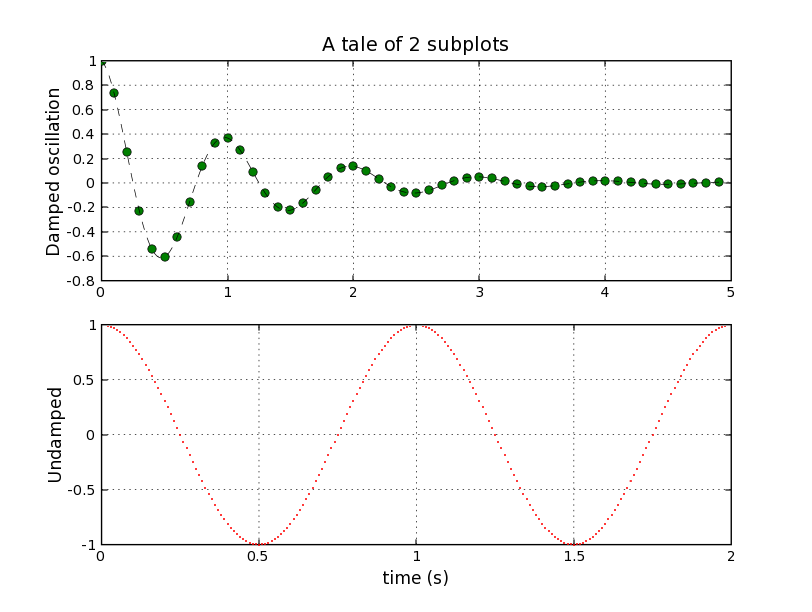
\includegraphics[width=4in]{fig/mpl_subplot_demo}
\par\end{centering}

\caption{\label{fig:mpl_subplot}It's easy to create multiple axes and subplots.}

\end{figure}


In addition to creating multiple subplots, this example contains a
couple of new things. In the first plot command, the return value
is stored as \texttt{l1, l2} and the \texttt{set} command is used
to change a default line property. 

\begin{lyxcode}
l1,~l2~=~plot(t1,~f(t1),~'bo',~t2,~f(t2),~'k-{}-')

set(l1,~markerfacecolor='g')
\end{lyxcode}
\texttt{l1} and \texttt{l2} are \texttt{matplotlib.lines.Line2D} instances
and they are created by the \texttt{plot} command and added to the
current axes. This is the typical mode of operation of the axes plot
commands: they create a bunch of primitive objects (lines, polygons,
text, images), add them to the axes, and return them. In this example,
the line's \texttt{markerfacecolor} property is set with the \texttt{set}
command. In the next section, we'll look into matplotlibs \texttt{set}
and \texttt{get} introspection system and show how to use it to customize
your lines, polygons, text instances and images.


\section[set and get]{Set and get introspection}

Everything that goes into a matplotlib figure, including the \texttt{Figure}
itself, are all objects dervied from a single base class \texttt{Artist,}
and the pylab \texttt{set} and \texttt{get} commands provide a unified
way to configure them. Let's create a simple plot of random circles,
and use that to explore how \texttt{set} and get work. First the basic
plot -- we'll store the return value as lines. Note that \texttt{plot}
always returns a \textit{list} of lines; in the example above there
were two lines \texttt{l1} and \texttt{l2}, and in the example below
there is only a single element of the list lines. No matter: \texttt{set}
and \texttt{get} will work on a single instance or a sequence of instances

\lstinputlisting{snippets/mpl_plot_line.ipy}

%
\begin{figure}
\begin{centering}
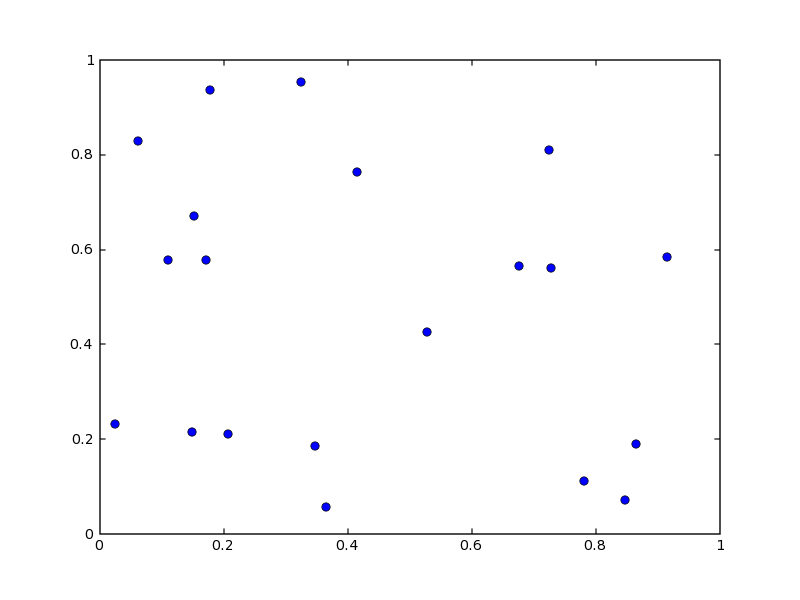
\includegraphics[width=4in]{fig/mpl_set_get1}
\par\end{centering}

\caption{\label{fig:mpl_setget1}The default marker plot, before marker customization}

\end{figure}


The simple figure that was created, a scattering of blue circles at
random locations, is shown in Figure\ref{fig:mpl_setget1}. To see
a listing of the properties of the line, and what their current values
are, call \texttt{get(lines)} \lstinputlisting{snippets/mpl_get.ipy}
and to see the same listing of properties with information on legal
values you can set them to, call \texttt{set(lines)}\lstinputlisting{snippets/mpl_set.ipy}

OK, we have a lot of options here.  Let's change the marker properties,
and add a linesytle

\begin{lyxcode}
In~{[}20]:~set(lines,~markerfacecolor='green',~markeredgecolor='red',

~~~....:~~markersize=20,~markeredgewidth=3,~

~~~....:~linestyle='-{}-',~linewidth=3)


\end{lyxcode}
That's a lot of typing, but to great effect!  The same data set now
has quite a different appearance, which is shown in Figure\ref{fig:mpl_setget2}.
Note in the long listing output of the set(lines) command above the
markerfacecolor settable property is listed as

\begin{lyxcode}
markerfacecolor~or~mfc:~any~matplotlib~color~-~see~help(colors)
\end{lyxcode}
The \texttt{markerfacecolor} has an alias \texttt{mfc} to save typing,
and common colornames have abbreviations too, so the \texttt{set}
command above could just as well be written

\begin{lyxcode}
In~{[}20]:~set(lines,~mfc='g',~mec='r',~ms=20,~mew=3,~ls='-{}-',~lw=3)

%
\begin{figure}
\begin{centering}
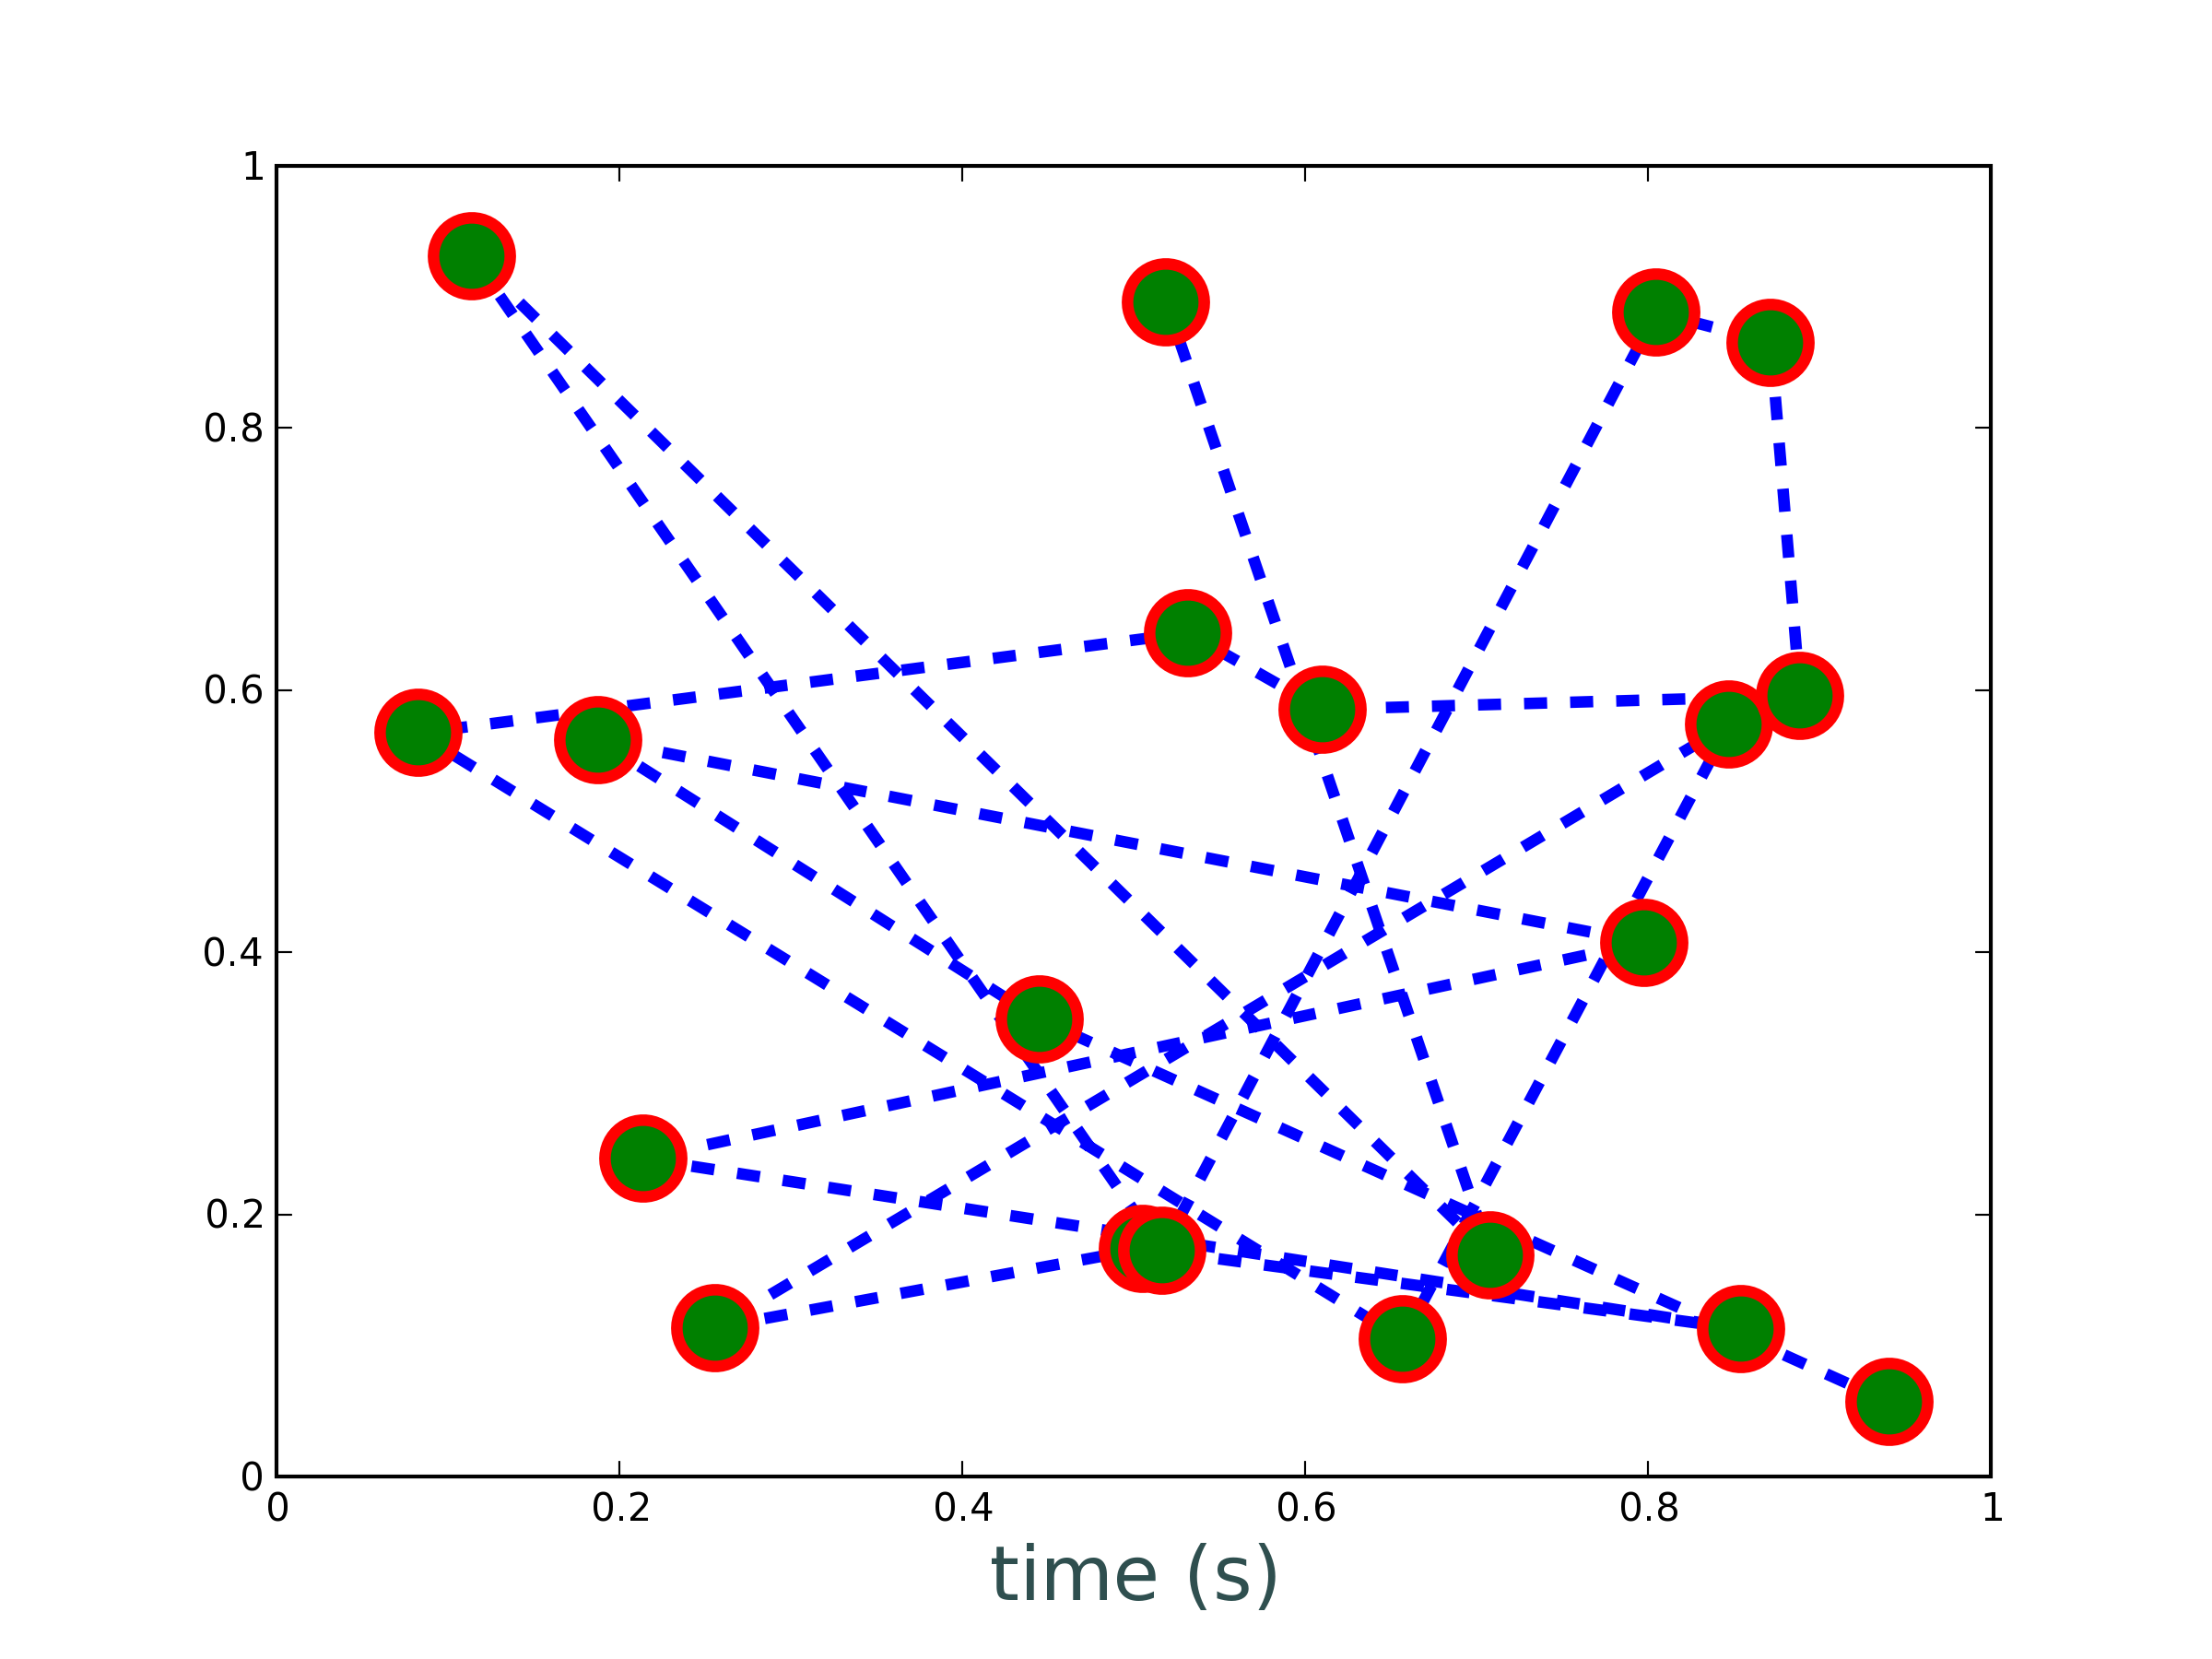
\includegraphics[width=4in]{fig/mpl_set_get2}
\par\end{centering}

\caption{\label{fig:mpl_setget2}The default marker plot, before marker customization}

\end{figure}

\end{lyxcode}
Another nice thing about matplotlib properties is that you can pass
them in as keyword arguments to \texttt{plot} and they will have the
same effect, eg, you can create the identical plot with

\begin{lyxcode}


In~{[}6]:~plot(x,~y,~'o',~mfc='g',~mec='r',~ms=20,~mew=3,~ls='-{}-',~lw=3)

Out{[}6]:~{[}<matplotlib.lines.Line2D~instance~at~0xb40db42c>]


\end{lyxcode}
As noted above, \texttt{set} and \texttt{get} work on any \texttt{Artist},
so you can configure your axes or text instances this way.  Eg, \texttt{xlabel}
returns a \texttt{matplotlib.text.Text} instance \lstinputlisting{snippets/mpl_text_set.ipy}

\begin{lyxcode}

\end{lyxcode}
So you have a lot of possibilities to customize your text!  The most
common things people what to do are change the font size and color;
the results of this command on the xlabel are shown in Figure\ref{fig:mpl_setget2}.

\begin{lyxcode}


In~{[}25]:~set(t,~fontsize=20,~color='darkslategray')~
\end{lyxcode}


\section[matplotlibrc]{Customizing the default behavior with the rc file}

matplotlib is designed to work in a variety of settings: some people
use it in \char`\"{}batch mode\char`\"{} on a web server to create
images they never look at. Others use graphical user interfaces (GUIs)
to interact with their plots. Thus you must customize matplotlib to
work like you want it to with the customization file \texttt{.matplotlibrc},
in which you can set whether you want to just create images or use
a GUI (the backend setting), and whether you want to work interactively
from the shell (the interactive setting). Almost all of the matplotlib
settings and figure properties can be customized with this file, which
is installed with the rest of the matplotlib data (fonts, icons, etc)
into a directory determined by distutils. Before compiling matplotlib,
it resides in the same dir as \texttt{setup.py} and will be copied
into your install path. Typical locations for this file are 

\begin{lyxcode}
C:\textbackslash{}Python23\textbackslash{}share\textbackslash{}matplotlib\textbackslash{}.matplotlibrc~\textcolor{blue}{\#~windows}~/usr/share/matplotlib/.matplotlibrc~~\textcolor{blue}{\#~linux}
\end{lyxcode}

By default, the installer will overwrite the existing file in the install path,
so if you want to preserve yours, please move it to your \texttt{HOME} dir and
set the environment variable if necessary.  In the rc file, you can set your
backend, whether you'll be working interactively and default values for most of
the figure properties.

In the RC file, blank lines, or lines starting with a comment symbol,
are ignored, as are trailing comments. Other lines must have the format

\begin{lyxcode}
~key~:~val~\textcolor{blue}{\#~optional~comment}~
\end{lyxcode}
where \textit{key} is some property like \texttt{backend}, \texttt{lines.linewidth},
or \texttt{figure.figsize} and \textit{val} is the value of that property.
Example entries for these properties are

\begin{lyxcode}
\textcolor{blue}{\#~this~is~a~comment~and~is~ignored~}

backend~~~~~~~~~:~GTKAgg~~~~\textcolor{blue}{\#~the~default~backend~}

lines.linewidth~:~0.5~~~~~~~\textcolor{blue}{\#~line~width~in~points}~

figure.figsize~~:~8,~6~~~~~~\textcolor{blue}{\#~figure~size~in~inches~}
\end{lyxcode}
A complete sample rc file is included with the matplotlib distribution
and available online.%
\footnote{http://matplotlib.sourceforge.net/.matplotlibrc%
}


\section[Plot Types]{A quick tour of plot types}


\section{Images}

Matplotlib has support for plotting images with imshow and figimage.
In imshow, the image data is scaled to fit into the current axes,
and many different interpolation schemes are supported to do the resampling,
and in figimage, the image data are transferred as a raw pixel dump
to the figure canvas without resampling. You can add colorbars, set
the default colormaps, and change the interpolation schemes quite
easily. 

%
\begin{figure}
\begin{centering}
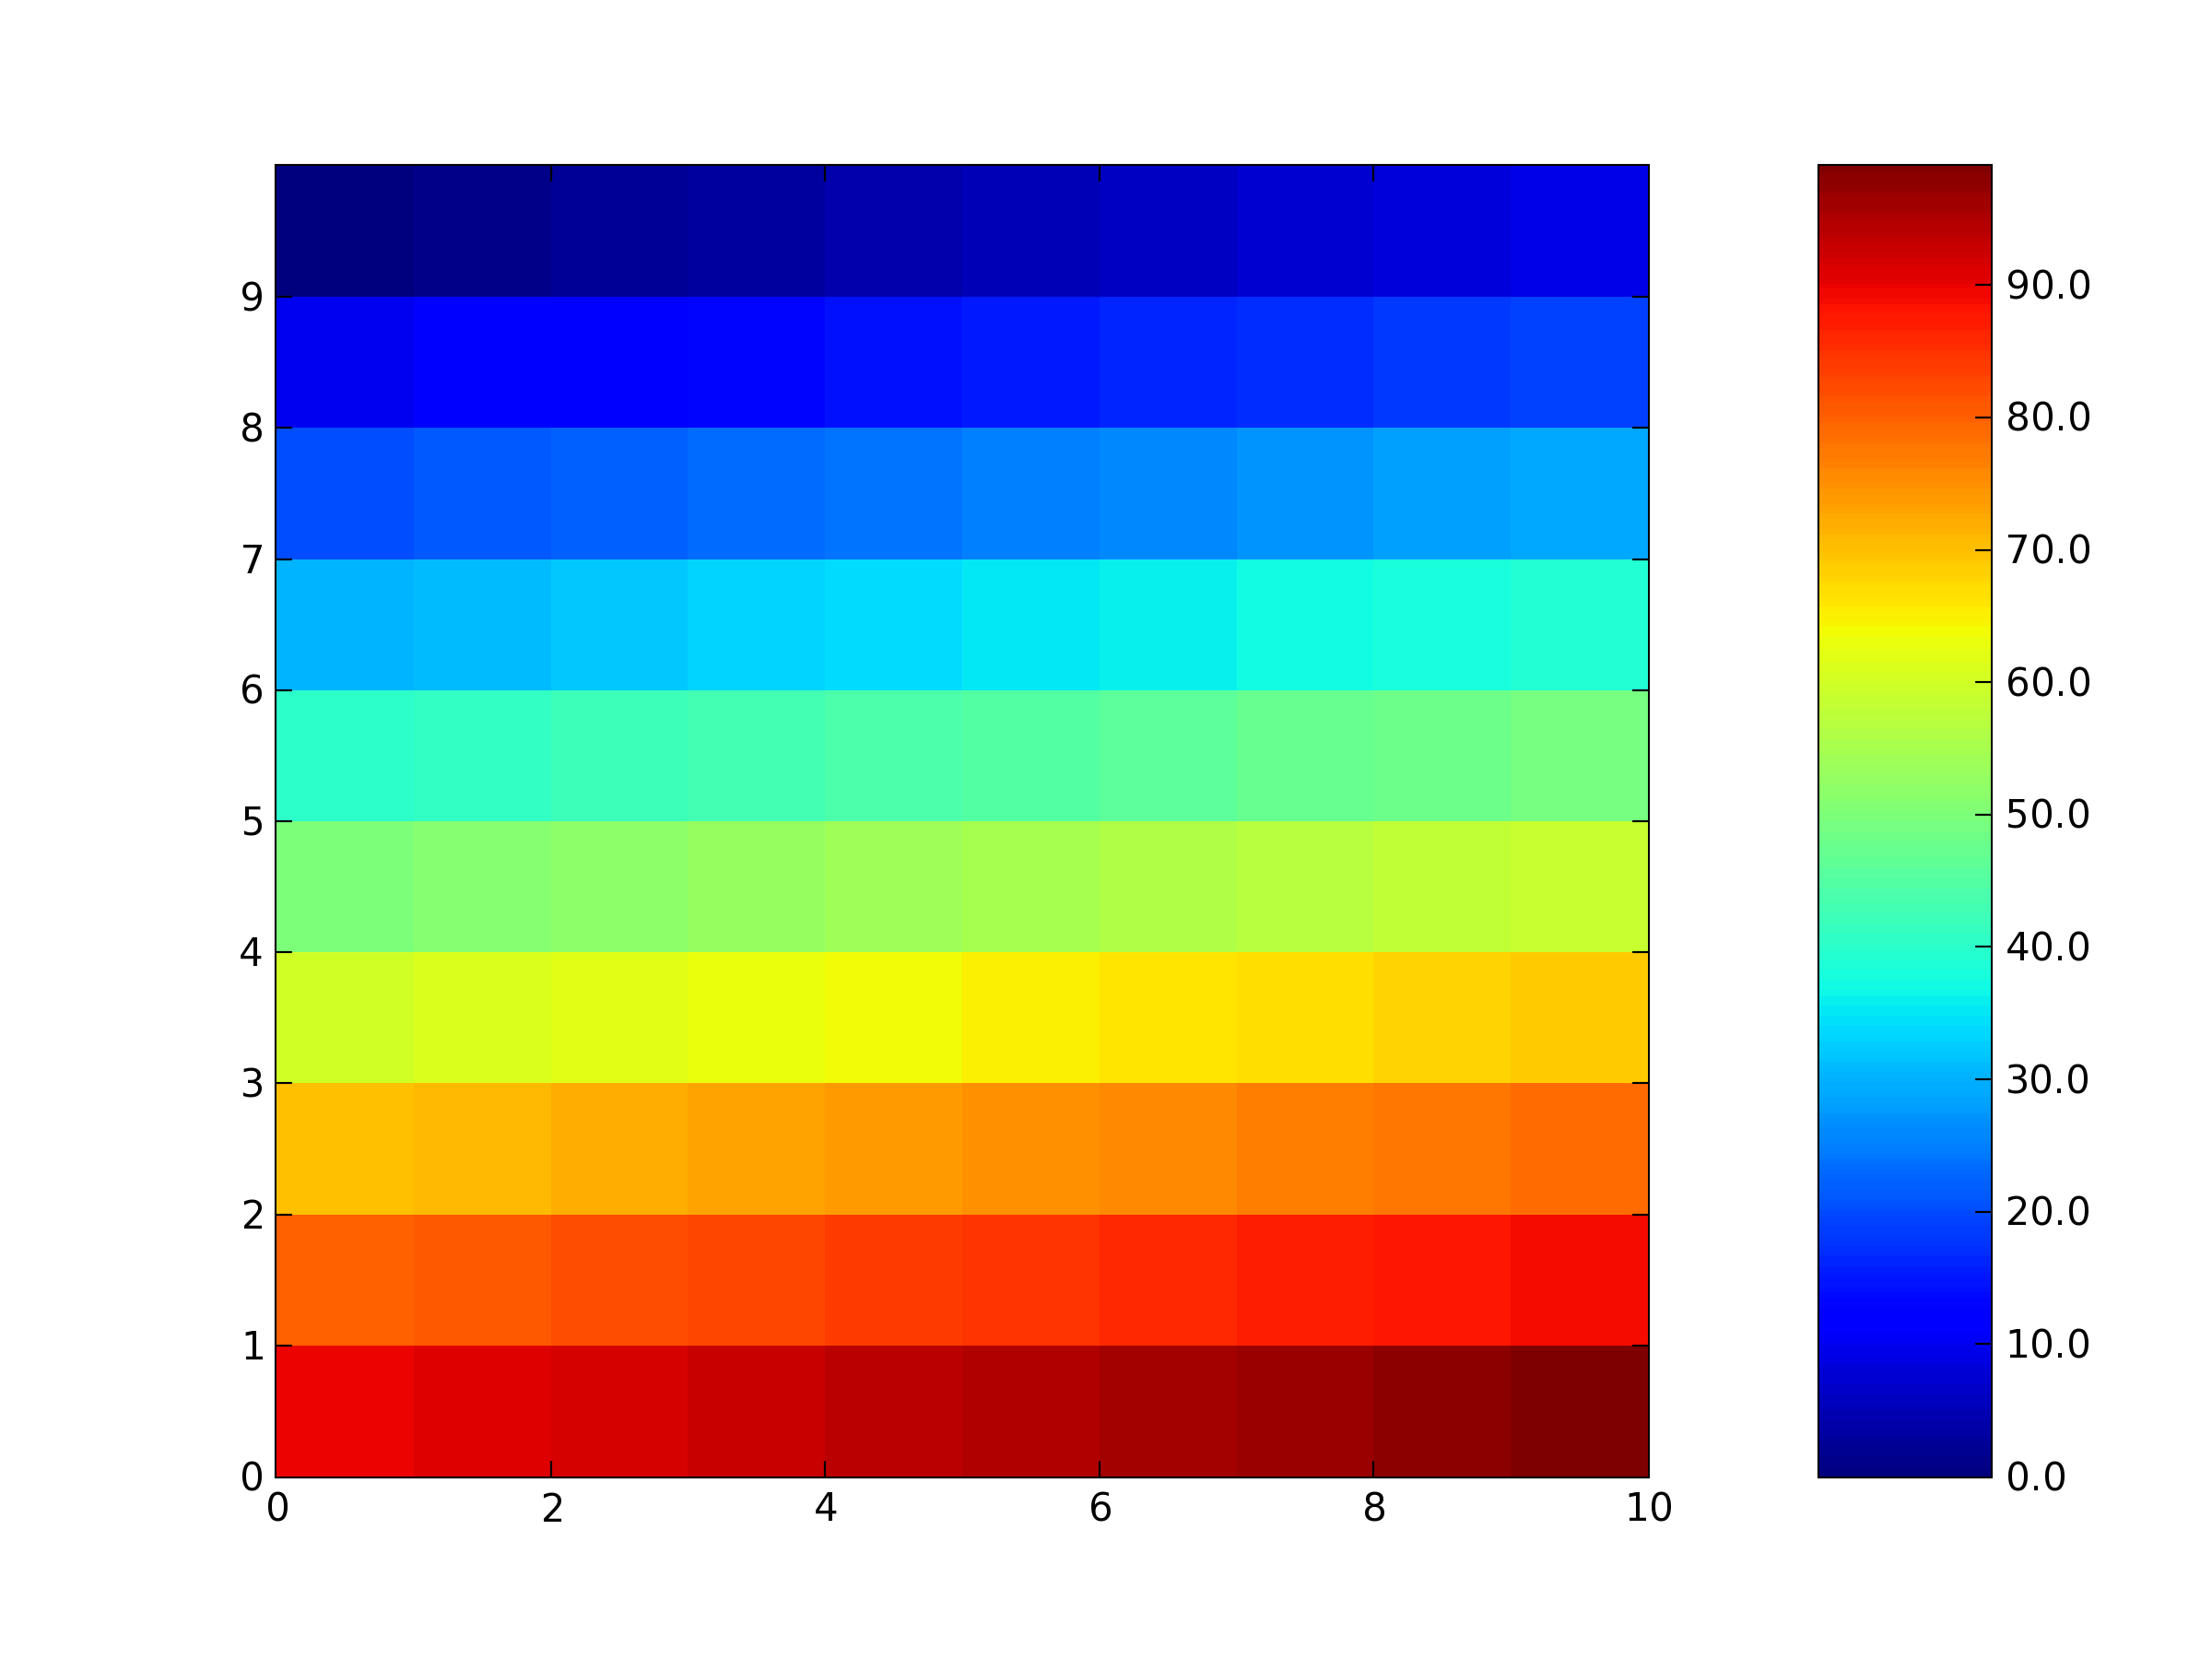
\includegraphics[width=4in]{fig/mpl_image_jet}
\par\end{centering}

\caption{\label{fig:mpl_imshow_jet}A simple image plot of a 2D matrix, using
nearest neighbor interpolation and the \texttt{jet} colormap.}

\end{figure}


\begin{lyxcode}
In~{[}15]:~x~=~arange(100.0);~x.shape~=~10,10

~

In~{[}16]:~im~=~imshow(x,~interpolation='nearest')

~

In~{[}17]:~colorbar()

Out{[}17]:~<matplotlib.axes.Axes~instance~at~0xb455496c>
\end{lyxcode}
which creates the image shown in Figure \ref{fig:mpl_imshow_jet}.
 You can interactively update the default colormap and change the
interpolation scheme, which creates the image show in Figure \ref{fig:mpl_imshow_hot}.

\begin{lyxcode}
In~{[}18]:~im.set\_interpolation('bilinear')

~

In~{[}19]:~hot()

%
\begin{figure}
\begin{centering}
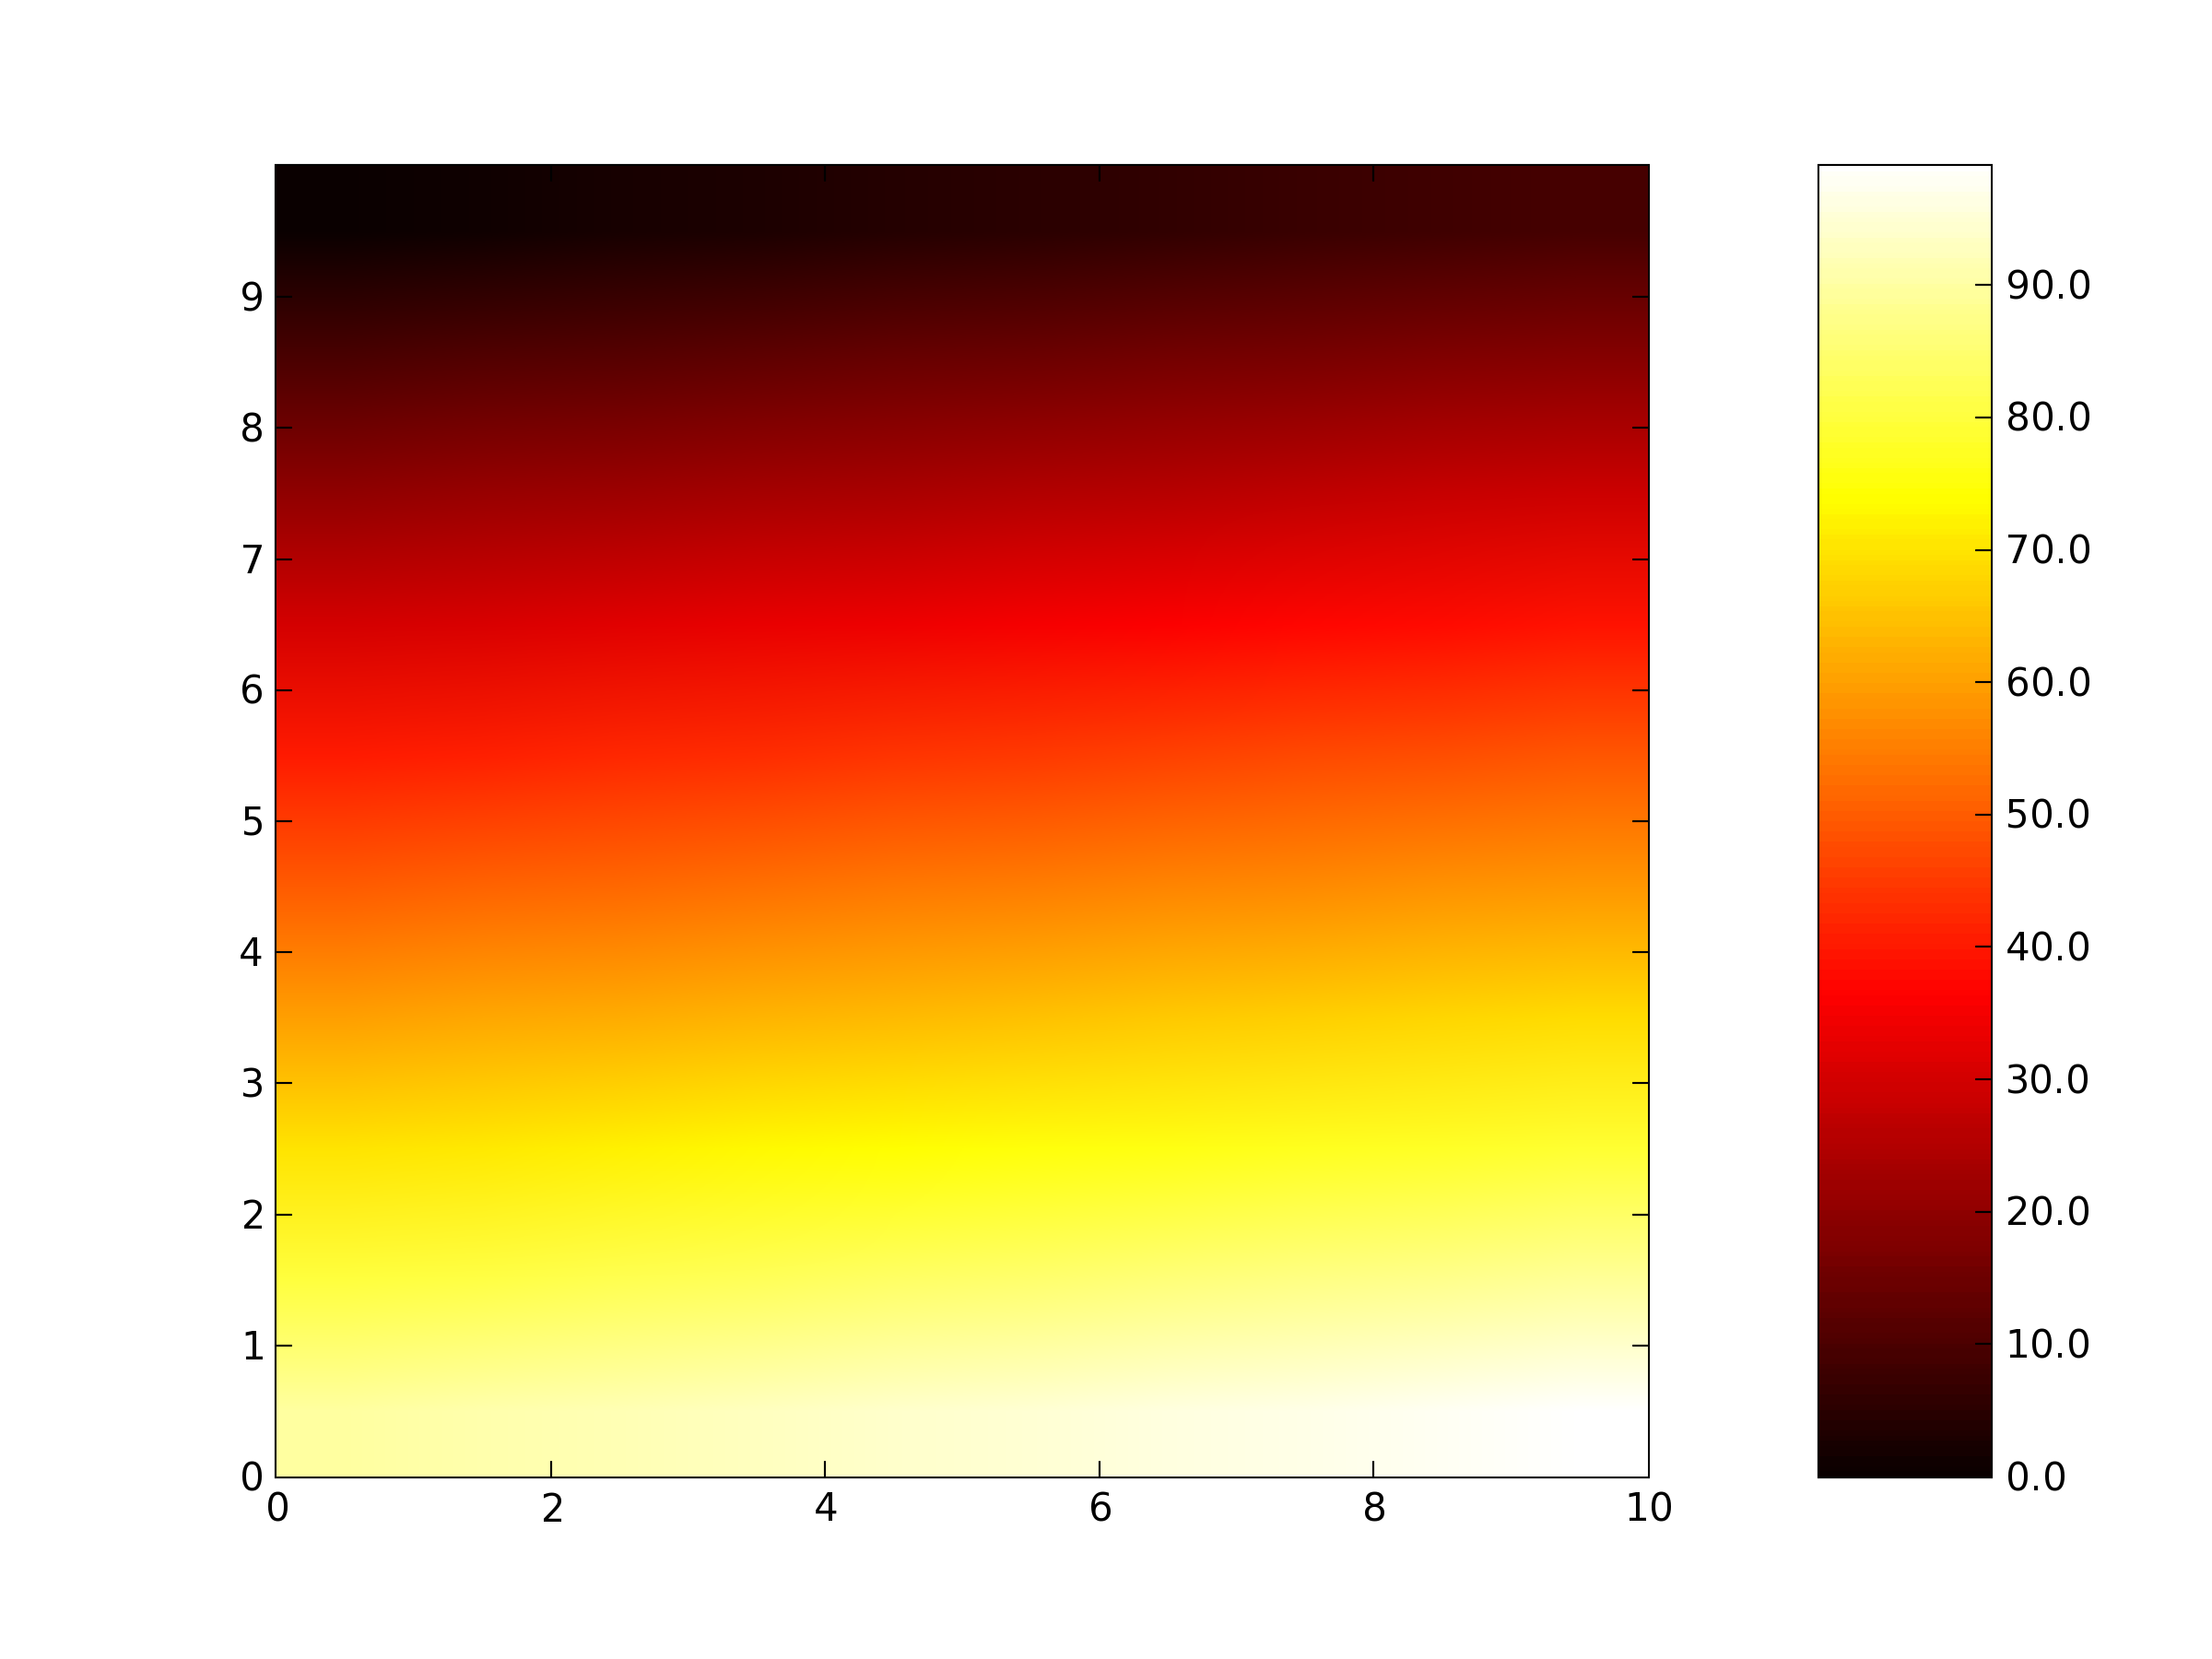
\includegraphics[width=4in]{fig/mpl_image_hot}
\par\end{centering}

\caption{\label{fig:mpl_imshow_hot}The same image data, rendered with the
hot colormap and bilinear interpolation. matplotlib has 14 colormaps
built-in, and you can define your own with relative ease, and there
are 16 interpolation methods.}

\end{figure}

\end{lyxcode}
There is a lot more you can do with images: you can set the data extent
so that you can overlay contours or other plots, you can plot multiple
images to the same axes with different colors and transparency values,
you can load images with PIL or \texttt{imread} and plot them in matplotlib,
you can create montages of with \texttt{figimage} placed around the
figure window at different offsets, you can plot grayscale, rgb or
rgba data, and so on.  Consult the \textit{Matplotlib User's Guide}
and the \texttt{examples} subdirectory in the matplotlib source distribution
for more information. We'll clost off with a simple example of reading
in a PNG and displaying it

\begin{lyxcode}
In~{[}35]:~im~=~imread('../data/ratner.png')

~

In~{[}36]:~imshow(im)

Out{[}36]:~<matplotlib.image.AxesImage~instance~at~0xb3ffba2c>

~

In~{[}37]:~axis('off')

%
\begin{figure}
\begin{centering}
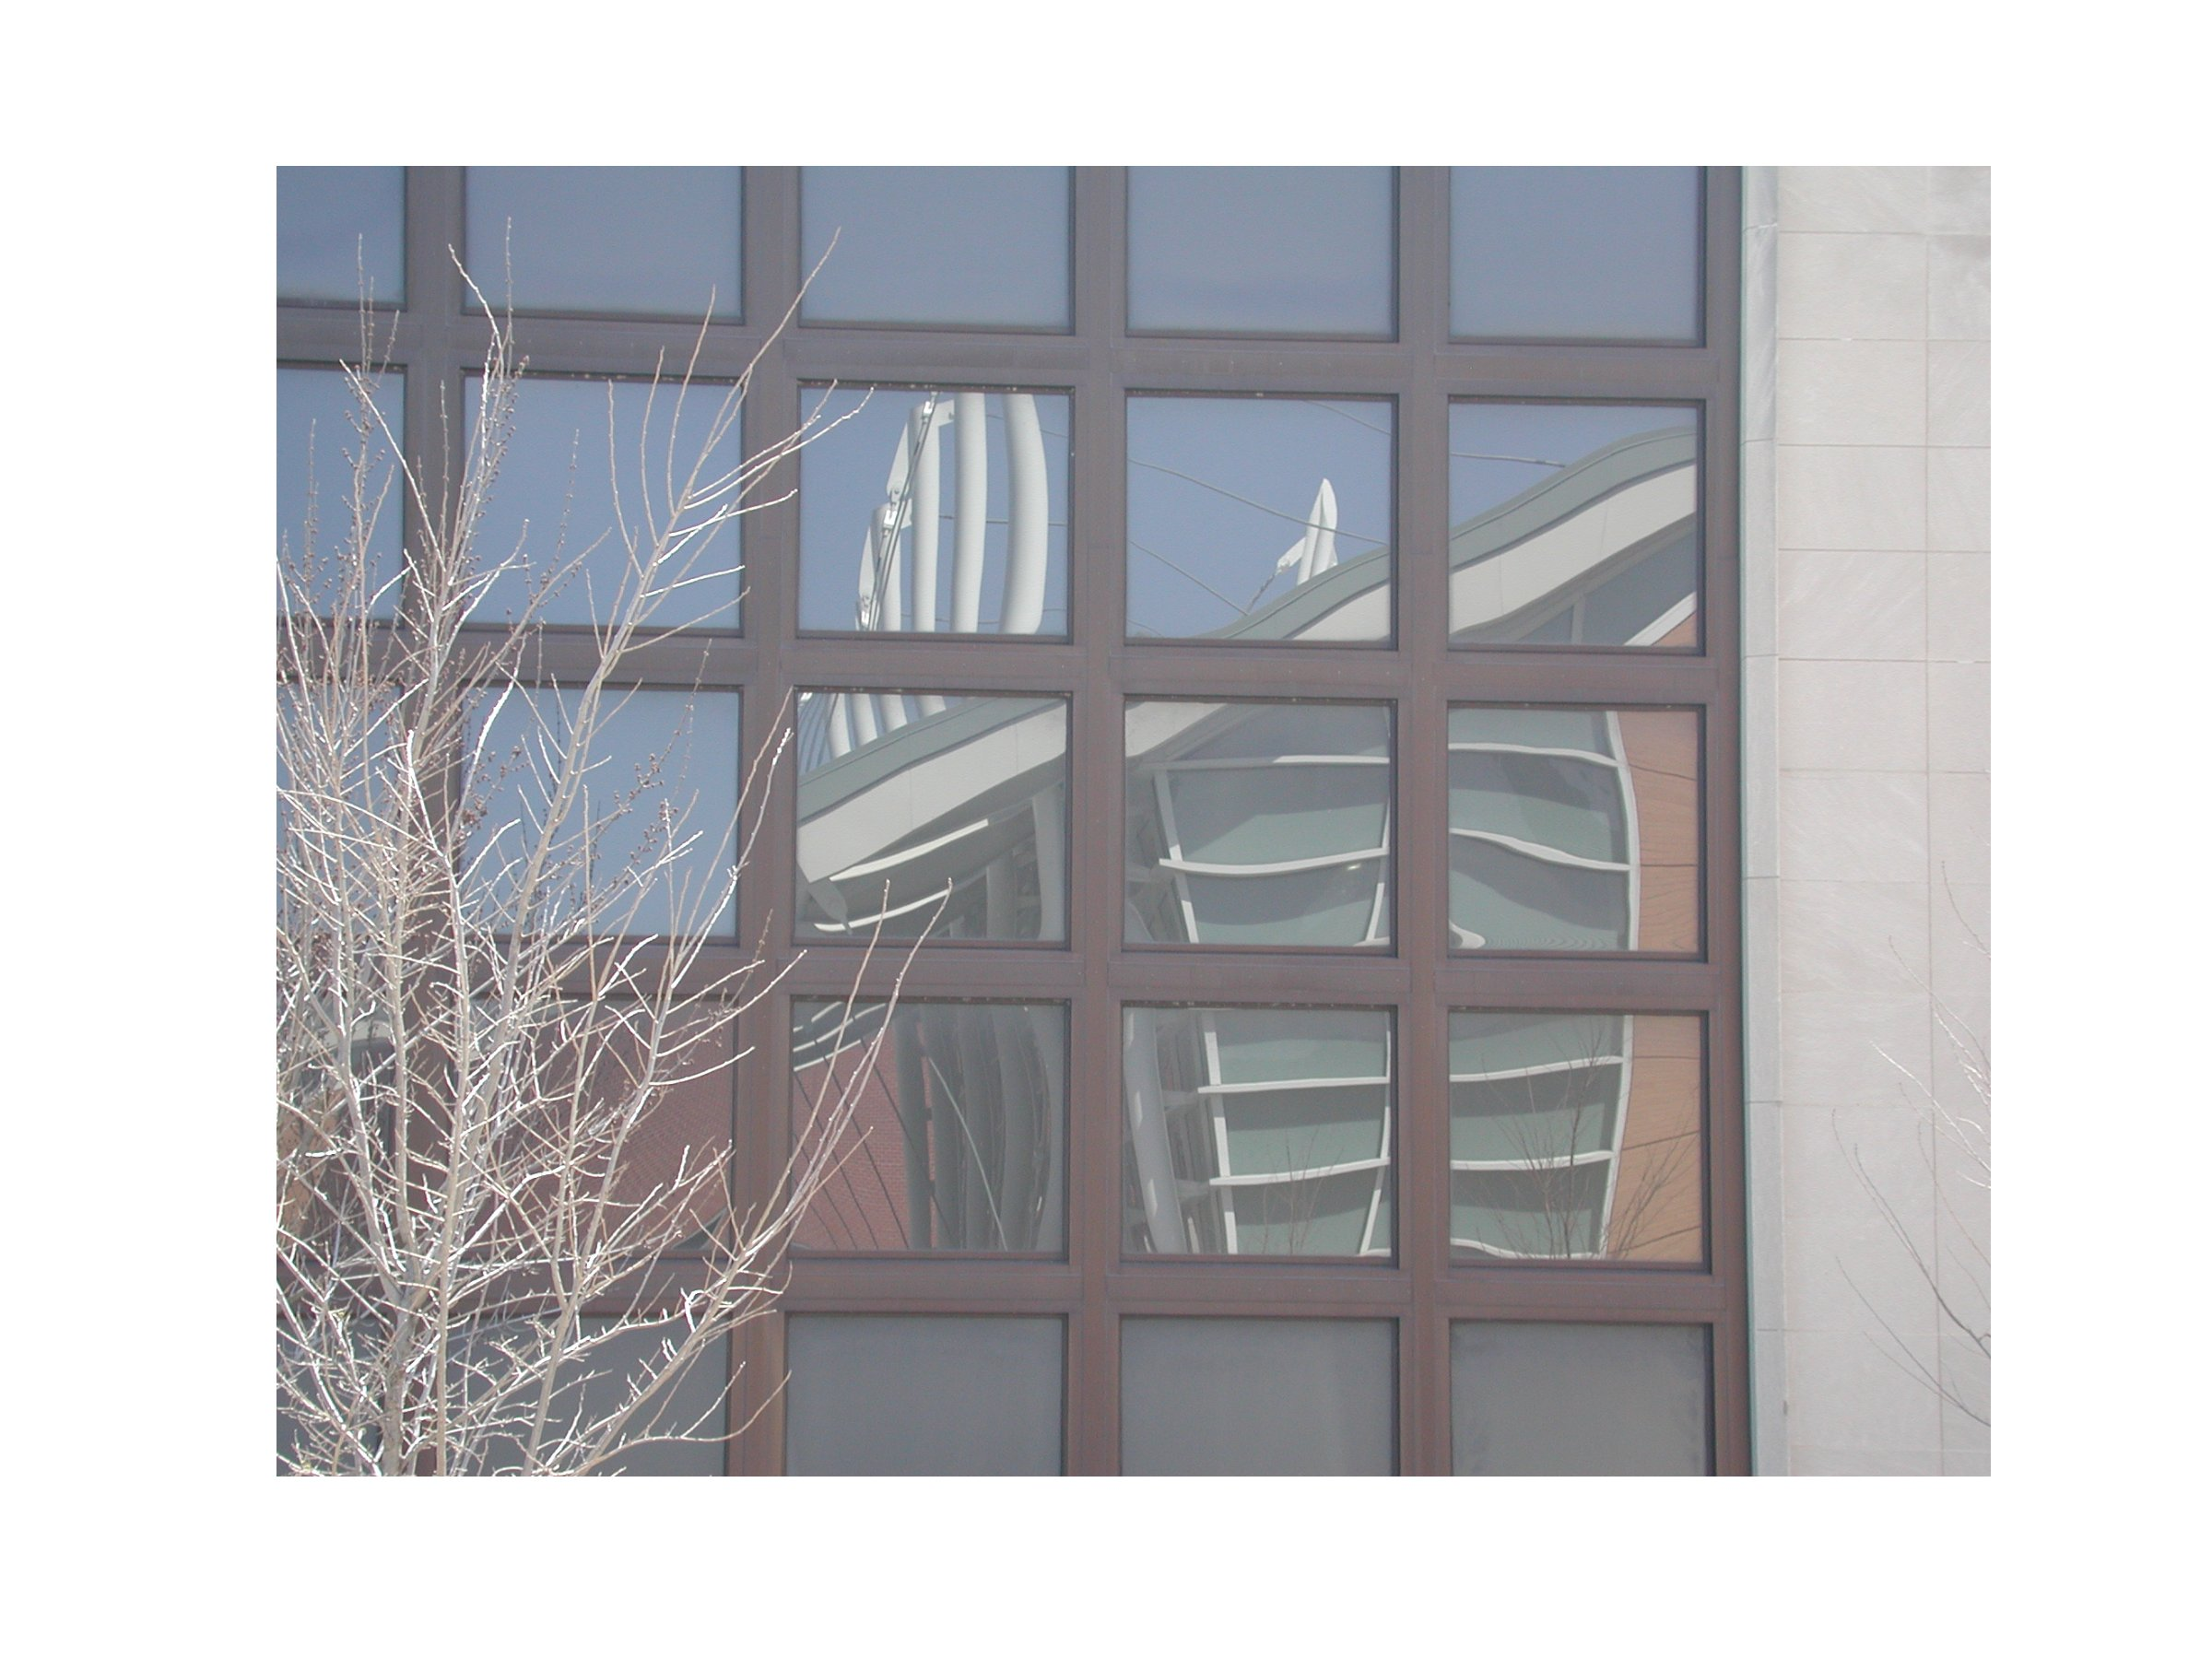
\includegraphics[width=5in]{fig/mpl_ratner}
\par\end{centering}

\caption{\label{fig:mpl_ratner}Displaying image data from your camera in matplotlib}

\end{figure}

\end{lyxcode}

\section[Text]{Customizing text and mathematical expressions}


\section[Event]{Event handling: Tracking the mouse and keyboard}



\chapter[External libraries]{Interfacing with external libraries}


\section{weave}

% John - should we talk to Eric Jones about letting us use parts of his weave
% docs? There's a very old set of docs for weave, I could update some of it and
% this would make an excellent section. Weave is really amazing, but badly
% under-documented and hence unknown.

Below is a listing of examples of weave use. This needs a lot of cleaning,
as some of this code is very old and doesn't actually run with current
weave. 

\lstinputlisting{examples/wrap_weave.py}


\section{swig }


\section{f2py }

This is a rough set of notes on how to use f2py. It does NOT substitute
the official manual, but is rather meant to be used alongside with
it. 

For any non-trivial poject involving f2py, one should also keep at
hand Pierre Schnizer's excellent 'A short introduction to F2PY', available
from http://fubphpc.tu-graz.ac.at/\textasciitilde{}pierre/f2py\_tutorial.tar.gz 


\subsection{Usage for the impatient }

Start by building a scratch signature file automatically from your
Fortran sources (in this case all, you can choose only those .f files
you need): 

\begin{lyxcode}
f2py~-m~MODULENAME~-h~MODULENAME.pyf~{*}.f~
\end{lyxcode}
This writes the file MODULENAME.pyf, making the best guesses it can
from the Fortran sources. It builds an interface for the module to
be accessed as 'import adap1d' from python.

You will then edit the .pyf file to fine-tune the python interface
exhibited by the resulting extension. This means for example making
unnecessary scratch areas or array dimensions hidden, or making certain
parameters be optional and take a default value.

Then, write your setup.py file using distutils, and list the .pyf
file along with the Fortran sources it is meant to wrap. f2py will
build the module for you automatically, respecting all the interface
specifications you made in the .pyf file.

This approach is ultimately far easier than trying to get all the
declarations (especially dependencies) right through Cf2py directives
in the Fortran sources. While that may seem appealing at first, experience
seems to show that it's ultimately far more time-consuming and prone
to subtle errors. Using this approach, the first f2py pass can do
the bulk of the interface writing and only fine-tuning needs to be
done manually. I would only recommend embedded Cf2py directives for
very simple problems (where it works very well).

The only drawback of this approach is that the interface and the original
Fortran source lie in different files, which need to be kept in sync.
This increases a bit the chances of forgetting to update the .pyf
file if the Fortran interface changes (adding a parameter, for example).
However, the benefit of having explicit, clear control over f2py's
behavior far outweighs this concern. 


\subsection{Choosing a default compiler }

Set the FC\_VENDOR environment variable. This will then prevent f2py
from testing all the compilers it knows about. 


\subsection{Using Cf2py directives }

For simpler cases you may choose to go the route of Cf2py directives.
Below are some tips and examples for this approach.

Here's the signature of a simple Fortran routine: \lstinputlisting[language=Fortran]{snippets/wrap_sub_sig.f}

The above is correctly handled by f2py, but it can't know what is
meant to be input/output and what the relations between the various
variables are (such as integers which are array dimensions). If we
add the following f2py directives, the generated python interface
is a lot nicer: \lstinputlisting[language=Fortran]{snippets/wrap_sub_sig_f2py.f}



Some comments on the above:

\begin{itemize}
\item The f2py directives should come immediately after the 'subroutine'
line and before the Fortran variable lines. This allows the f2py dimension
directives to override the Fortran var({*}) directives.
\item If the Fortran code uses var(N) instead of var({*}), the f2py directives
can be placed after the Fortran declarations. This mode is preferred,
as there is less redundancy overall. The result is much simpler: 
\end{itemize}
\lstinputlisting[language=Fortran]{snippets/wrap_sub_sig_f2py.f}



Since python can automatically manage memory, it is possible to hide
the need for manually passed 'work' areas. The C/python wrapper to
the underlying fortran routine will allocate the memory for the needed
work areas on the fly. This is done by specifying intent(hide,cache).
'hide' tells f2py to remove the variable from the argument list and
'cache' tells it to auto-generate it.

In cases where the allocation cost becomes a performance problem,
one can remove the 'hide' part and make it an optional argument. In
this case it will only be generated if not given. For this, the line
above should be changed to:

\begin{lyxcode}
{\small Cf2py~~~real~{*}8~dimension(2{*}mm+2),~intent(cache),~optional,~depend(mm)~::~wrk~}{\small \par}
\end{lyxcode}
Note that this should only be done after proving that the scratch
areas are causing a performance problem. The \texttt{cache} directive
causes f2py to keep cached copies of the scratch areas, so no unnecessary
mallocs should be triggered.

Since f2py relies on NumPy arrays, all dimensions can be determined from the
arrays themselves and it is not necessary to pass them explicitly.

With all this, the resulting f2py-generated docstring becomes: 

\begin{lyxcode}
phipol~-~Function~signature:

~~phi~=~phipol(j,nodes,wei,x)

Required~arguments:

~~j~:~input~int

~~nodes~:~input~rank-1~array('d')~with~bounds~(mm)

~~wei~:~input~rank-1~array('d')~with~bounds~(mm)

~~x~:~input~rank-1~array('d')~with~bounds~(nn)

Return~objects:

~~phi~:~rank-1~array('d')~with~bounds~(nn)
\end{lyxcode}

\subsection{Debugging}

For debugging, use the --debug-capi option to f2py. This causes the
extension modules to print detailed information while in operation.
In distutils, this must be passed as an option in the f2py\_options
to the Extension constructor. 


\subsection{Wrapping C codes with f2py}

Below is Pearu Peterson's (the f2py author) response to a question
about using f2py to wrap existing C codes. While SWIG provides similar
functionality and weave is perfect for inlining C, f2py seems to be
an incredibly simple and convenient tool for wrapping C libraries.

Pearu's response follows: 

For example, consider the following C file:

\begin{lyxcode}
/{*}~foo.c~{*}/

double~foo(double~{*}x,~int~n)~\{

~~int~i;

~~double~r~=~0;

~~for~(i=0;i<n;++i)

~~~~r~+=~x{[}i];

~~return~r;

\}

/{*}~EOF~foo.c~{*}/
\end{lyxcode}
To wrap the C function foo() with f2py, create the following signature
file bar.pyf: 

\begin{lyxcode}
!~-{*}-~F90~-{*}-

python~module~bar

~~interface

~~~~real{*}8~function~foo(x,n)

~~~~~~intent(c)~foo

~~~~~~real{*}8~dimension(n),intent(in)~::~x

~~~~~~integer~intent(c,hide),depend(x)~::~n~=~len(x)

~~~~end~function~foo

~~end~interface

end~python~module~bar

!~EOF~bar.pyf
\end{lyxcode}
(see usersguide for more info about intent(c)) and run

\begin{lyxcode}
~~f2py~-c~bar.pyf~foo.c
\end{lyxcode}
Finally, in Python:

\begin{lyxcode}
>\,{}>\,{}>~import~bar

>\,{}>\,{}>~bar.foo({[}1,2,3])

6.0
\end{lyxcode}

\subsection{Passing offset arrays to Fortran routines}

It is possible to pass offset arrays (like pointers to the middle
of other arrays) by using NumPy's slice notation.

The print\_dvec function below simply prints its argument as \char`\"{}print{*},'x',x\char`\"{}.
We show some examples of how it behaves with both 1 and 2-d arrays: 

\begin{lyxcode}
In~{[}3]:~x

Out{[}3]:~array({[}~2.8,~~3.4,~~4.1])

In~{[}4]:~tf.print\_dvec(x)

~n~3

~x~~2.8~~3.4~~4.1

In~{[}5]:~tf.print\_dvec~?

Type:~~~~~~~~~~~fortran

String~Form:~~~~<fortran~object~at~0x8306fe8>

Namespace:~~~~~~Currently~not~defined~in~user~session.

Docstring:

~~~~print\_dvec~-~Function~signature:

~~~~~~print\_dvec(x,{[}n])

~~~~Required~arguments:

~~~~~~x~:~input~rank-1~array('d')~with~bounds~(n)

~~~~Optional~arguments:

~~~~~~n~:=~len(x)~input~int

In~{[}6]:~tf.print\_dvec~(x{[}1])

~n~1

~x~~3.4

In~{[}7]:~tf.print\_dvec~(x{[}1:])

~n~2

~x~~3.4~~4.1

In~{[}8]:~A

Out{[}8]:

array({[}{[}~3.5,~~5.6,~~8.2],

~~~~~~~{[}~2.1,~~4.5,~~1.2],

~~~~~~~{[}~6.3,~~3.4,~~3.1]])

In~{[}9]:~tf.print\_dvec(A)

~n~9

~x~~3.5~~5.6~~8.2~~2.1~~4.5~~1.2~~6.3~~3.4~~3.1

In~{[}10]:~A

Out{[}10]:

array({[}{[}~3.5,~~5.6,~~8.2],

~~~~~~~{[}~2.1,~~4.5,~~1.2],

~~~~~~~{[}~6.3,~~3.4,~~3.1]])

In~{[}11]:~tf.print\_dvec(A{[}1:])

~n~6

~x~~2.1~~4.5~~1.2~~6.3~~3.4~~3.1

In~{[}12]:~A{[}1:]

Out{[}12]:

array({[}{[}~2.1,~~4.5,~~1.2],

~~~~~~~{[}~6.3,~~3.4,~~3.1]])

In~{[}13]:~A{[}1:,1:]

Out{[}13]:

array({[}{[}~4.5,~~1.2],

~~~~~~~{[}~3.4,~~3.1]])

In~{[}14]:~tf.print\_dvec(A{[}1:,1:])

~n~4

~x~~4.5~~1.2~~3.4~~3.1
\end{lyxcode}

\subsection{On matrix ordering and in-memory copies}

NumPy (which f2py relies on) is C-based, and therefore its arrays
are stored in row-major order. Fortran stores its arrays in column-major
order. This means that copying issues must be dealt with. Below we
reproduce some comments from Pearu on this topic given in the f2py
mailing list in June/2002: 

\begin{quote}
To avoid copying, you should create array that has internally Fortran
data ordering. This is achived, for example, by reading/creating your
data in Fortran ordering to NumPy array and then doing numpy.transpose
on that. Every f2py generated extension module provides also function 

has\_column\_major\_storage

to check if an array is Fortran contiguous or not. If has\_column\_major\_storage(arr)
returns true then there will be no copying for the array arr if passed
to f2py generated functions (assuming that the types are proper, of
cource).

Also note that copying done by f2py generated interface is carried
out in C on the raw data and therefore it is extremely fast compared
to if you would make a copy in Python, even when using NumPy. Tests
with say 1000x1000 matrices show that there is no noticable performance
hit when copying is carried out, in fact, sometimes making a copy
may speed up things a bit -- I was quite surprised about that myself.

So, I think, you should worry about copying only if the sizes of matrices
are really large, say, larger than 5000x5000 and efficient memory
usage is relevant. The time spent for copying is negligible even for
large arrays provided that your computer has plenty of memory (>=256MB).
\end{quote}

\subsection{Distutils}

Below is an example setup.py file which generates a Python extension
module from Fortran90 sources and a .pyf interface file generated
by f2py and later fine tuned. 

\lstinputlisting{examples/wrap_f2py_setup.py}


\section{Others}

boost, pyrex, cxx


\section[Standalone applications]{Distributing standalone applications}

py2exe, mcmillan installer




\part{Workbook}

% This part specifies the chapter declarations in the main file, while the
% chapters are made of individual TeX files which themselves should be written
% at the section level.  The idea is for each chapter to be focused on one or a
% few closely related topics, and to allow users to build them with as many or
% as few actual sections as desired for a given audience.

\chapter{Introduction}

This document contains a set of small problems, drawn from many different
fields, meant to illustrate commonly useful techniques for using Python
in scientific computing.

All problems are presented in a similar fashion: the task is explained
including any necessary mathematical background and a `code skeleton'
is provided that is meant to serve as a starting point for the solution
of the exercise. In some cases, some example output of the expected
solution, figures or additional hints may be provided as well. 

The accompanying source download for this workbook contains the complete
solutions, which are not part of this document for the sake of brevity.

For several examples, the provided skeleton contains pre-written tests
which validate the correctness of the expected answers. When you have
completed the exercise successfully, you should be able to run it
from within IPython and see something like this (illustrated using
a trapezoidal rule problem, whose solution is in the file \texttt{trapezoid.py}):

\begin{lstlisting}
In [7]: run trapezoid.py
....
----------------------------------------------------------------------
Ran 4 tests in 0.003s

OK
\end{lstlisting}

This message tells you that 4 automatic tests were successfully executed.
The idea of including automatic tests in your code is a common one
in modern software development, and Python includes in its standard
library two modules for automatic testing, with slightly different
functionality: \texttt{unittest} and \texttt{doctest}. These tests
were written using the \texttt{unittest} system, whose complete documentation
can be found here: \url{http://docs.python.org/lib/module-unittest.html}. 

Other exercises will illustrate the use of the \texttt{doctest} system,
since it provides complementary functionality.


\chapter{Simple non-numerical problems}


\section{Sorting quickly with QuickSort }

Quicksort is one of the best known, and probably the simplest, fast
algorithm for sorting $n$ items. It is fast in the sense that it
requires on average $\mathcal{O}(n\log n)$ comparisons instead of
$\mathcal{O}(n^{2})$, although a naive implementation does have quadratic
worst-case behavior.

The algorithm uses a simple divide and conquer strategy, and its implementation
is naturally recursive. Its basic steps are:

\begin{enumerate}
\item Pick an element from the list, called the pivot $p$ (any choice works).
\item Select from the rest of the list those elements smaller and those
greater than the pivot, and store them in separate lists $S$ and
$G$.
\item Recursively apply the algorithm \texttt{}to $S$ and $G$. The final
result can be written as $\sigma(S)+[p]+\sigma(G)$, where $\sigma$
represents the sorting operation, $+$ indicates list concatenation
and $[p]$ is the list containing the pivot as its single element.
\end{enumerate}
The listing~\ref{code:qsort} contains a skeleton with no implementation
but with tests already written (in the form of \emph{unit tests},
as described in the introduction).

\lstinputlisting[label=code:qsort,caption={IGNORED}]{problems/qsort.py}


\subsection*{Hints}

\begin{itemize}
\item Python has no particular syntactic requirements for implementing recursion,
but it does have a maximum recursion depth. This value can be queried
via the function \texttt{sys.getrecursionlimit()}, and it can be changed
with \texttt{sys.setrecursionlimit(new\_value)}. 
\item Like in all recursive problems, don't forget to implement an exit
condition!
\item If \texttt{L} is a list, the call \texttt{len(L)} provides its length.
\end{itemize}




\section{Dictionaries for counting words}

A common task in text processing is to produce a count of word frequencies.
While NumPy has a builtin histogram function for doing numerical histograms,
it won't work out of the box for couting discrete items, since it
is a binning histogram for a range of real values.

But the Python language provides very powerful string manipulation
capabilities, as well as a very flexible and efficiently implemented
builtin data type, the \emph{dictionary}, that makes this task a very
simple one.

In this problem, you will need to count the frequencies of all the
words contained in a compressed text file supplied as input. 

The listing~\ref{code:wordfreqs} contains a skeleton for this
problem, with \texttt{XXX} marking various places that are incomplete. 

\lstinputlisting[label=code:wordfreqs,caption={IGNORED}]{problems/wordfreqs.py}


\subsection*{Hints}

\begin{itemize}
\item The \texttt{print\_vk} function is already provided for you as a simple
way to summarize your results.
\item You will need to read the compressed file \texttt{HISTORY.gz}. Python
has facilities to do this without having to manually uncompress it.
\item Consider `words' simply the result of splitting the input text into
a list, using any form of whitespace as a separator. This is obviously
a very na�ve definition of `word', but it shall suffice for the purposes
of this exercise.
\item Python strings have a \texttt{.split()} method that allows for very
flexible splitting. You can easily get more details on it in IPython:
\end{itemize}
\begin{lstlisting}
In [2]: a = 'somestring'

In [3]: a.split?
Type:           builtin_function_or_method
Base Class:     <type 'builtin_function_or_method'>
Namespace:      Interactive
Docstring:
    S.split([sep [,maxsplit]]) -> list of strings

    Return a list of the words in the string S, using sep as the
    delimiter string.  If maxsplit is given, at most maxsplit
    splits are done. If sep is not specified or is None, any
    whitespace string is a separator.
\end{lstlisting}

The complete set of methods of Python strings can be viewed by hitting
the TAB key in IPython after typing `\texttt{a.}', and each of them
can be similarly queried with the `\texttt{?}' operator as above.
For more details on Python strings and their companion sequence types,
see \url{http://docs.python.org/lib/typesseq.html}.


\chapter{Working with files, the internet, and numpy arrays}

This section is a general overview to show how easy it is to load
and manipulate data on the file system and over the web using python's
built in data structures and numpy arrays.  The goal is to exercise
basic programming skills like building filename or web addresses to
automate certain tasks like loading a series of data files or
downloading a bunch of related files off the web, as well as to
illustrate basic numpy and pylab skills.

\section{Loading and saving ASCII data}
\label{sec:ascii_data}

The simplest file format is a plain text ASCII file of numbers.
Although there are many better formats out there for saveing and
loading data, this format is extremely common because it has the
advantages of being human readable, and thus will survive the test of
time as the \textit{en vogue} programming languages, analysis
applications and data formats come and go, it is easy to parse, and it
is supported by almost all languages and applications.  

In this exercise we will create a data set of two arrays, the first
one regularly sampled time \textit{t} from 0..2 seconds with 20~ms
time step , and the second one an array \texttt{v} of sinusoidal
voltages corrupted by some noise.  Let's assume the sine wave has
amplitude 2~V, frequency 10~Hz, and zero mean Gaussian distrubuted
white noise with standard deviation 0.5~V.  Your task is to write two
scripts.

The first script should create the vectors \texttt{t} and \texttt{v},
plot the time series of \texttt{t} versus \texttt{v}, save them in a
two dimensional numpy array \texttt{X}, and then dump the array
\texttt{X} to a plain text ASCII file called
\texttt{'noisy\_sine.dat'}.  The file will look like (not identical
because of the noise)

\begin{verbatim}
0.000000000000000000e+00 1.550947826934816025e-02
2.000000000000000042e-02 2.493944587057004725e+00
4.000000000000000083e-02 9.497694074551737975e-01
5.999999999999999778e-02 -9.185779287524413750e-01
8.000000000000000167e-02 -2.811127590689064704e+00
... and so on
\end{verbatim}

Here is the exercise skeleton of the script to create and plot the
data file

\lstinputlisting[label=code:noisy_sine,caption={IGNORED}]{problems/noisy_sine.py}

and the graph will look something like Figure~\ref{fig:noisy_sine}

\begin{center}%
\begin{figure}
\begin{centering}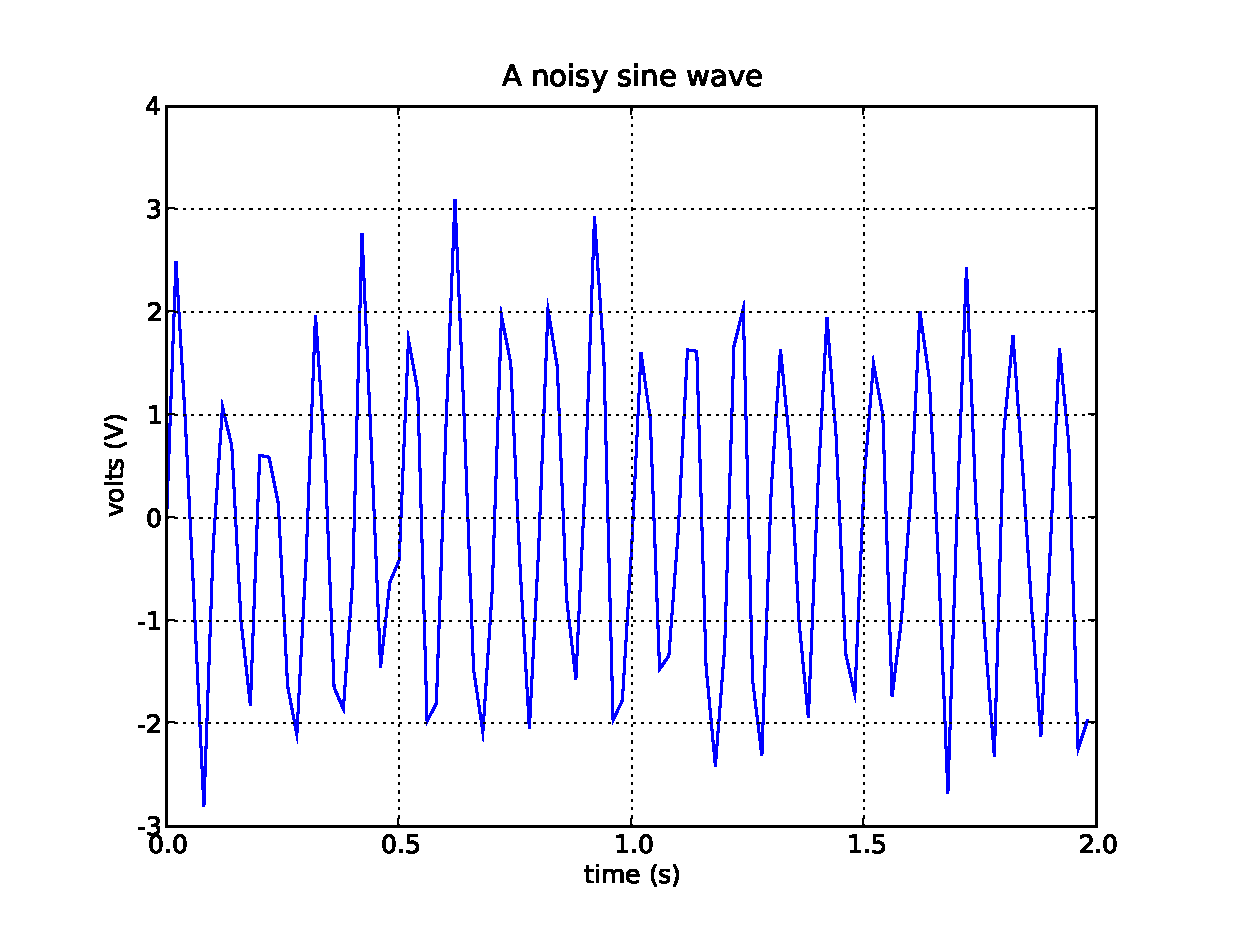
\includegraphics[width=4in]{fig/noisy_sine}\par\end{centering}


\caption{\label{fig:noisy_sine}A 10~Hz sine wave corrupted by noise}
\end{figure}
\par\end{center}


The second part of this exercise is to write a script which loads data
from the data file into an array \texttt{X}, extracts the columns into
arrays \texttt{t} and \texttt{v}, and computes the RMS
(root-mean-square) intensity of the signal using the \texttt{load}
command.

\section{Working with CSV files}

The CSV (Comma Separated Value) file specification is also an ASCII
based, human readable format, but it is more powerful than simple flat
ASCII files including headers, escape sequences and arbitrary
delimiters like TAB, SPACE or COMMA.  It is a widely used interchange
format for sharing data between operating systems and programs like
Excel, Matlab and statistical analysis packages.

A typical CSV file will be a mix of different data types: integers,
floating point numbers, dates and strings.  Of course, all of these
are strings in the file, since all text files are made up of strings,
but the data is typically representing some other numeric or date
type.  Python has very good support for handling different data types,
so you don't need to try to force your data to look like a multi
dimensional array of floating point numbers if this is not the natural
way to describe your data.  numpy provides a generalization of the
array data structure we used above called record arrays, which allow
to store data in a conceptual model similar to a database or
spreadsheet: several named fields (eg 'date', 'weight', 'height',
'age') with different types (eg \texttt{datetime.date}, \texttt{float},
\texttt{float}, \texttt{int}).

In the example below, we will download some CSV files from Yahoo
Financial web pages and load them into numpy record arrays for
analysis and visualization.  Go to \texttt{http://finance.yahoo.com}
and enter a stock symbol in the entry boc labeled ``Get Quotes''.  I
will use \texttt{'SPY'} which is an index fund that tracks the S\&P
500.  In the left menu bar, there is an entry called ``Historical
Prices'' which will take you to a page where you can download the
price history of your stock.  Near the bottom of this page you should
see a ``Download To Spreadsheet'' link -- instead of clicking on it,
right click it and choose ``Copy Link Location'' and paste this into a
python script or ipython session as a string named \texttt{url}.  Eg,
for SPY page better

\begin{lstlisting}
url = 'http://ichart.finance.yahoo.com/table.csv?' +\
   's=SPY&d=9&e=20&f=2007&g=d&a=0&b=29&c=1993&ignore=.csv'
\end{lstlisting}

\noindent I've broken the url into two strings so they will fit on the
page.  If you spend a little time looking at this pattern, you can
probably figure out what is going on.  The URL is encoding the
information about the stock, the variable \texttt{s} for the stock
ticker, \texttt{d} for the latest month, \texttt{e} for the latest
day, \texttt{f} for the latest year, \texttt{c} for the start year,
and so on (similarly \texttt{a}, \texttt{b}, and \texttt{c} for the
start month, day and year).  This is handy to know, because below we
will write some code to automate some downloads for a stock universe.

One of the great things about python is it's ``batteries included''
standard library, which includes support for dates, csv files and
internet downloads.  The example interactive session below shows how
in just a few lines of code using python's \texttt{urllib} for
retrieving information from the internet, and matplotlib's
\texttt{csv2rec} function for loading numpy record arrays, we are
ready to get to work analyzing some web based data.  Comments have
been added to a copy-and-paste from the interactive session

\begin{lstlisting}
# import a couple of libraries we'll be needing
In [23]: import urllib
In [24]: import matplotlib.mlab as mlab

# this is the CSV file we'll be downloading
In [25]: url = 'http://ichart.finance.yahoo.com/table.csv?' +\
   's=SPY&d=9&e=20&f=2007&g=d&a=0&b=29&c=1993&ignore=.csv'

# this will grab that web file and save it as 'SPY.csv' on our local
# filesystem
In [27]: urllib.urlretrieve(url, 'SPY.csv')
Out[27]: ('SPY.csv', <httplib.HTTPMessage instance at 0x2118210>)

# here we use the UNIX command head to peak into the file, which is
# a comma separated and contains various types, dates, ints, floats
In [28]: !head SPY.csv
Date,Open,High,Low,Close,Volume,Adj Close
2007-10-19,153.09,156.48,149.66,149.67,295362200,149.67
2007-10-18,153.45,154.19,153.08,153.69,148367500,153.69
2007-10-17,154.98,155.09,152.47,154.25,216687300,154.25
2007-10-16,154.41,154.52,153.47,153.78,166525700,153.78
2007-10-15,156.27,156.36,153.94,155.01,161151900,155.01
2007-10-12,155.46,156.35,155.27,156.33,124546700,156.33
2007-10-11,156.93,157.52,154.54,155.47,233529100,155.47
2007-10-10,156.04,156.44,155.41,156.22,101711100,156.22
2007-10-09,155.60,156.50,155.03,156.48,94054300,156.48

# csv2rec will import the file into a numpy record array, inspecting
# the columns to determine the correct data type
In [29]: r = mlab.csv2rec('SPY.csv')

# the dtype attribute shows you the field names and data types.  
# O4 is a 4 byte python object (datetime.date), f8 is an 8 byte 
# float, i4 is a 4 byte integer and so on.  The > and < symbols
# indicate the byte order of multi-byte data types, eg big endian or
# little endian, which is important for cross platform binary data
# storage
In [30]: r.dtype
Out[30]: dtype([('date', '|O4'), ('open', '>f8'), ('high', '>f8'),
('low', '>f8'), ('close', '>f8'), ('volume', '>i4'), ('adj_close',
'>f8')])

# Each of the columns is stored as a numpy array, but the types are 
# preserved.  Eg, the adjusted closing price column adj_close is a
# floating  point type, and the date column is a python datetime.date
In [31]: print r.adj_close
[ 149.67  153.69  154.25 ...,   34.68   34.61   34.36]
In [32]: print r.date
[2007-10-19 00:00:00 2007-10-18 00:00:00 2007-10-17 00:00:00 ...,
 1993-02-02 00:00:00 1993-02-01 00:00:00 1993-01-29 00:00:00]
\end{lstlisting}

For your exercise, you'll elaborate on the code here to do a batch
download of a number of stock tickers in a defined stock universe.
Define a function \texttt{fetch\_stock(ticker)} which takes a stock
ticker symbol as an argument and returns a numpy record array.  Select
the rows of the record array where the date is greater than 2003-01-01
and plot the returns $(p-p_0)/p_0$ where $p$ are the prices and $p_0$
is the initial price. by date for each stock on the same plot.  Create
a legend for the plot using the matplotlib \texttt{legend} command,
and print out a sorted list of final returns (eg assuming you bought
in 2003 and held to the present) for each stock.  Here is the exercise
skeleton.:

\lstinputlisting[label=code:stock_records,caption={IGNORED}]{problems/stock_records.py}

The graph will look something like Figure~\ref{fig:stock_records}.

\begin{center}%
\begin{figure}
\begin{centering}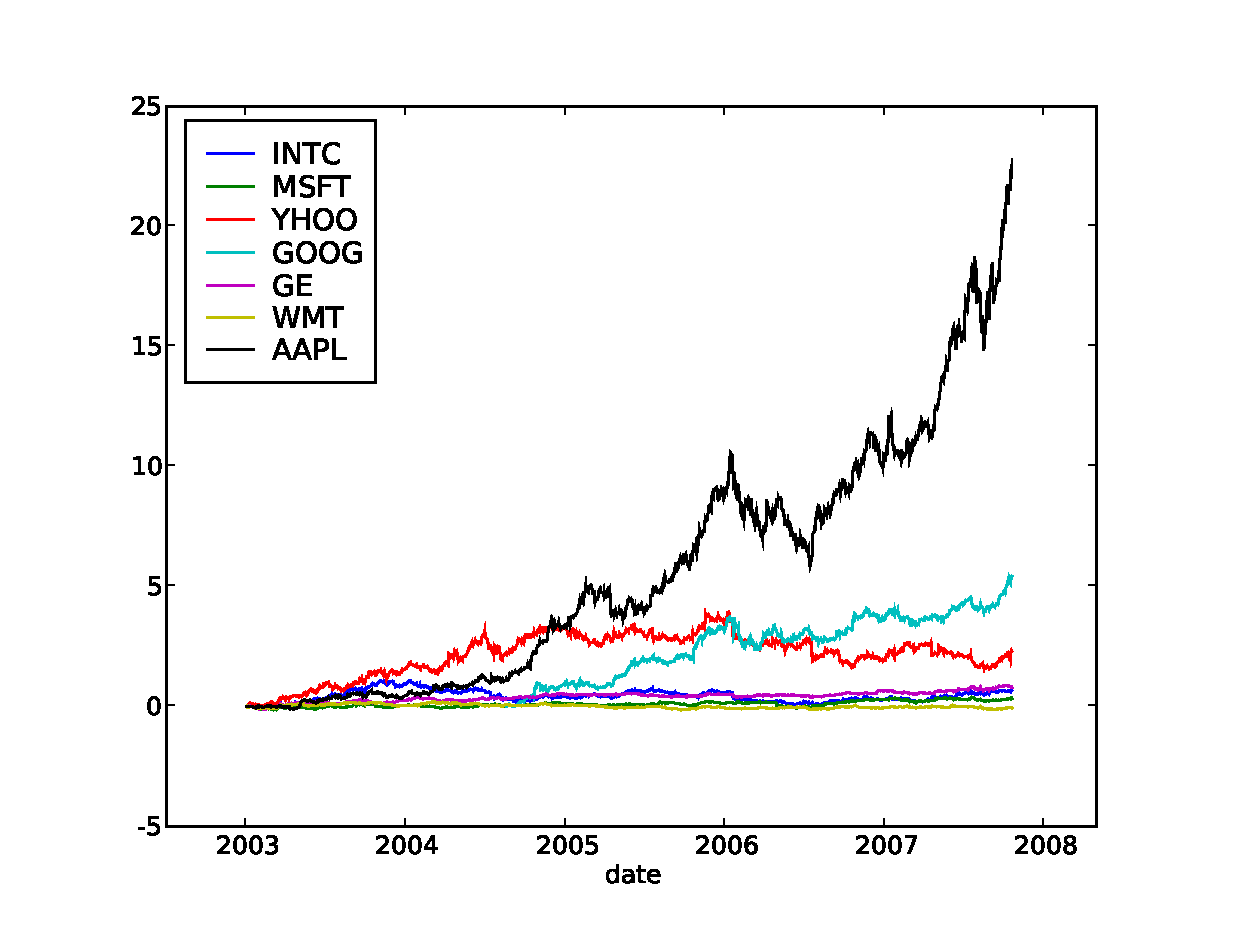
\includegraphics[width=4in]{fig/stock_records}\par\end{centering}


\caption{\label{fig:stock_records}Returns for a universe of stocks
  since 2003}
\end{figure}
\par\end{center}


\section{Loading and saving binary data}
\label{sec:binary_data}

ASCII is bloated and slow for working with large arrays, and so binary
data should be used if performance is a consideration.  To save an
array \texttt{X} in binary form, you can use the numpy
\texttt{tostring} method

\begin{lstlisting}
In [16]: import numpy

# create some random numbers
In [17]: x = numpy.random.rand(5,2)

In [19]: print x
[[ 0.56331918  0.519582  ]
 [ 0.22685429  0.18371135]
 [ 0.19384767  0.27367054]
 [ 0.35935445  0.95795884]
 [ 0.37646642  0.14431089]]

# save it to a data file in binary
In [20]: x.tofile(file('myx.dat', 'wb'))

# load it into a new array
In [21]: y = numpy.fromfile(file('myx.dat', 'rb'))

# the shape is not preserved, so we will have to reshape it
In [22]: print y
[ 0.56331918  0.519582    0.22685429  0.18371135  0.19384767
0.27367054
  0.35935445  0.95795884  0.37646642  0.14431089]

In [23]: y.shape
Out[23]: (10,)

# restore the original shape
In [24]: y.shape = 5, 2

In [25]: print y
[[ 0.56331918  0.519582  ]
 [ 0.22685429  0.18371135]
 [ 0.19384767  0.27367054]
 [ 0.35935445  0.95795884]
 [ 0.37646642  0.14431089]]
\end{lstlisting}

The advantage of numpy \texttt{tofile} and \texttt{fromfile} over
ASCII data is that the data storage is compact and the read and write
are very fast.  It is a bit of a pain that that meta ata like array
datatype and shape are not stored.  In this format, just the raw binary
numeric data is stored, so you will have to keep track of the data
type and shape by other means.  This is a good solution if you need to
port binary data files between different packages, but if you know you
will always be working in python, you can use the python pickle
function to preserve all metadata (pickle also works with all standard
python data types, but has the disadvantage that other programs and
applications cannot easily read it)

\begin{lstlisting}
# create a 6,3 array of random integers
In [36]: x = (256*numpy.random.rand(6,3)).astype(numpy.int)

In [37]: print x
[[173  38   2]
 [243 207 155]
 [127  62 140]
 [ 46  29  98]
 [  0  46 156]
 [ 20 177  36]]

# use pickle to save the data to a file myint.dat
In [38]: import cPickle

In [39]: cPickle.dump(x, file('myint.dat', 'wb'))

# load the data into a new array
In [40]: y = cPickle.load(file('myint.dat', 'rb'))

# the array type and share are preserved
In [41]: print y
[[173  38   2]
 [243 207 155]
 [127  62 140]
 [ 46  29  98]
 [  0  46 156]
 [ 20 177  36]]
\end{lstlisting}





\chapter{Elementary Numerics}


\section{Wallis' slow road to $\pi$}

Wallis' formula is an infinite product that converges (slowly) to
$\pi$:\begin{equation}
\pi=\prod_{i=1}^{\infty}\frac{4i^{2}}{4i^{2}-1}.\end{equation}


The listing~\ref{code:wallis_pi} contains a skeleton with no
implementation but with some plotting commands already inserted, so
that you can visualize the convergence rate of this formula as more
terms are kept.

\lstinputlisting[label=code:wallis_pi,caption={IGNORED}]{examples/wallis_pi.py}

After running the script successfully, you should obtain a plot similar
to Figure~\ref{fig:wallis_pi}.

\begin{center}%
\begin{figure}
\begin{centering}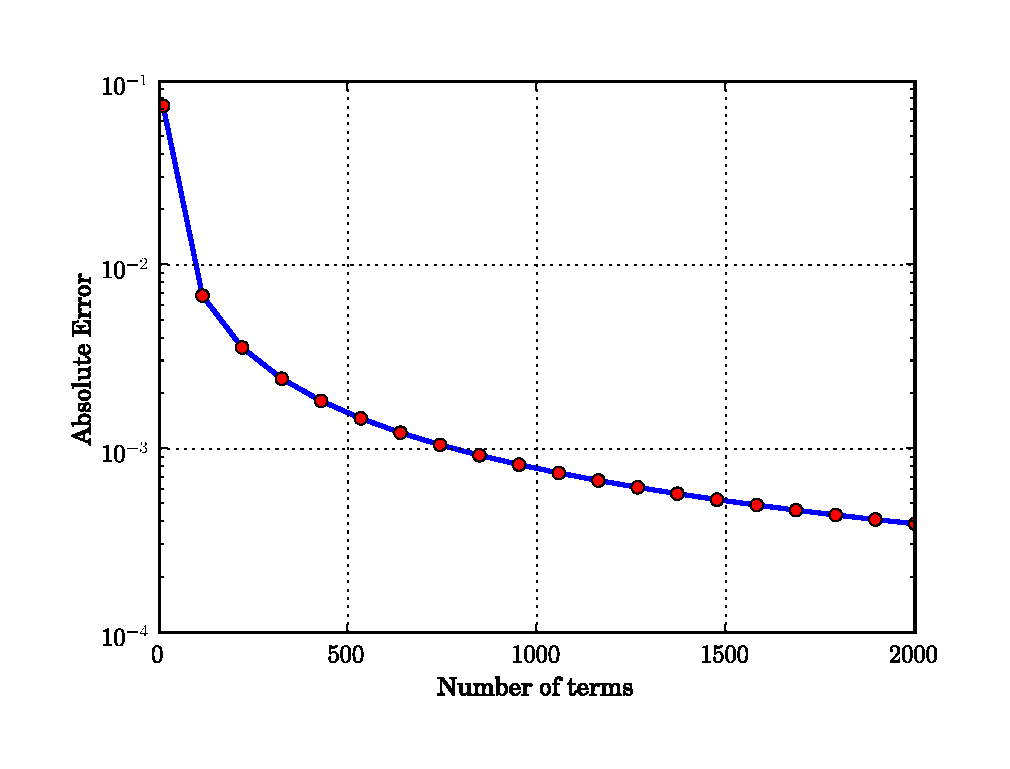
\includegraphics[width=4in]{fig/wallis_pi_convergence}\par\end{centering}


\caption{\label{fig:wallis_pi}Convergence rate for Wallis' infinite product
approximation to $\pi.$}
\end{figure}
\par\end{center}


\section{Trapezoidal rule}
\label{sec:trapezoid}

In this exercise, you are tasked with implementing the simple trapezoid
rule formula for numerical integration. If we want to compute the
definite integral \begin{equation}
\int_{a}^{b}f(x)dx\end{equation}
we can partition the integration interval $[a,b]$ into smaller subintervals,
and approximate the area under the curve for each subinterval by the
area of the trapezoid created by linearly interpolating between the
two function values at each end of the subinterval. This is graphically
illustrated in Figure~\ref{fig:trapezoid}, where the blue line represents
the function $f(x)$ and the red line represents the successive linear
segments.

The area under $f(x)$ (the value of the definite integral) can thus
be approximated as the sum of the areas of all these trapezoids. If
we denote by $x_{i}$ ($i=0,\ldots,n,$ with $x_{0}=a$ and $x_{n}=b$)
the abscissas where the function is sampled, then \begin{equation}
\int_{a}^{b}f(x)dx\approx\frac{1}{2}\sum_{i=1}^{n}\left(x_{i}-x_{i-1}\right)\left(f(x_{i})+f(x_{i+1})\right).\label{eq:trapzf}\end{equation}
The common case of using equally spaced abscissas with spacing $h=(b-a)/n$
reads simply \begin{equation}
\int_{a}^{b}f(x)dx\approx\frac{h}{2}\sum_{i=1}^{n}\left(f(x_{i})+f(x_{i+1})\right).\label{eq:trapzf2}\end{equation}
One frequently receives the function values already precomputed, $y_{i}=f(x_{i}),$
so equation~(\ref{eq:trapzf}) becomes \begin{equation}
\int_{a}^{b}f(x)dx\approx\frac{1}{2}\sum_{i=1}^{n}\left(x_{i}-x_{i-1}\right)\left(y_{i}+y_{i-1}\right).\label{eq:trapz}\end{equation}


%
\begin{figure}
\begin{centering}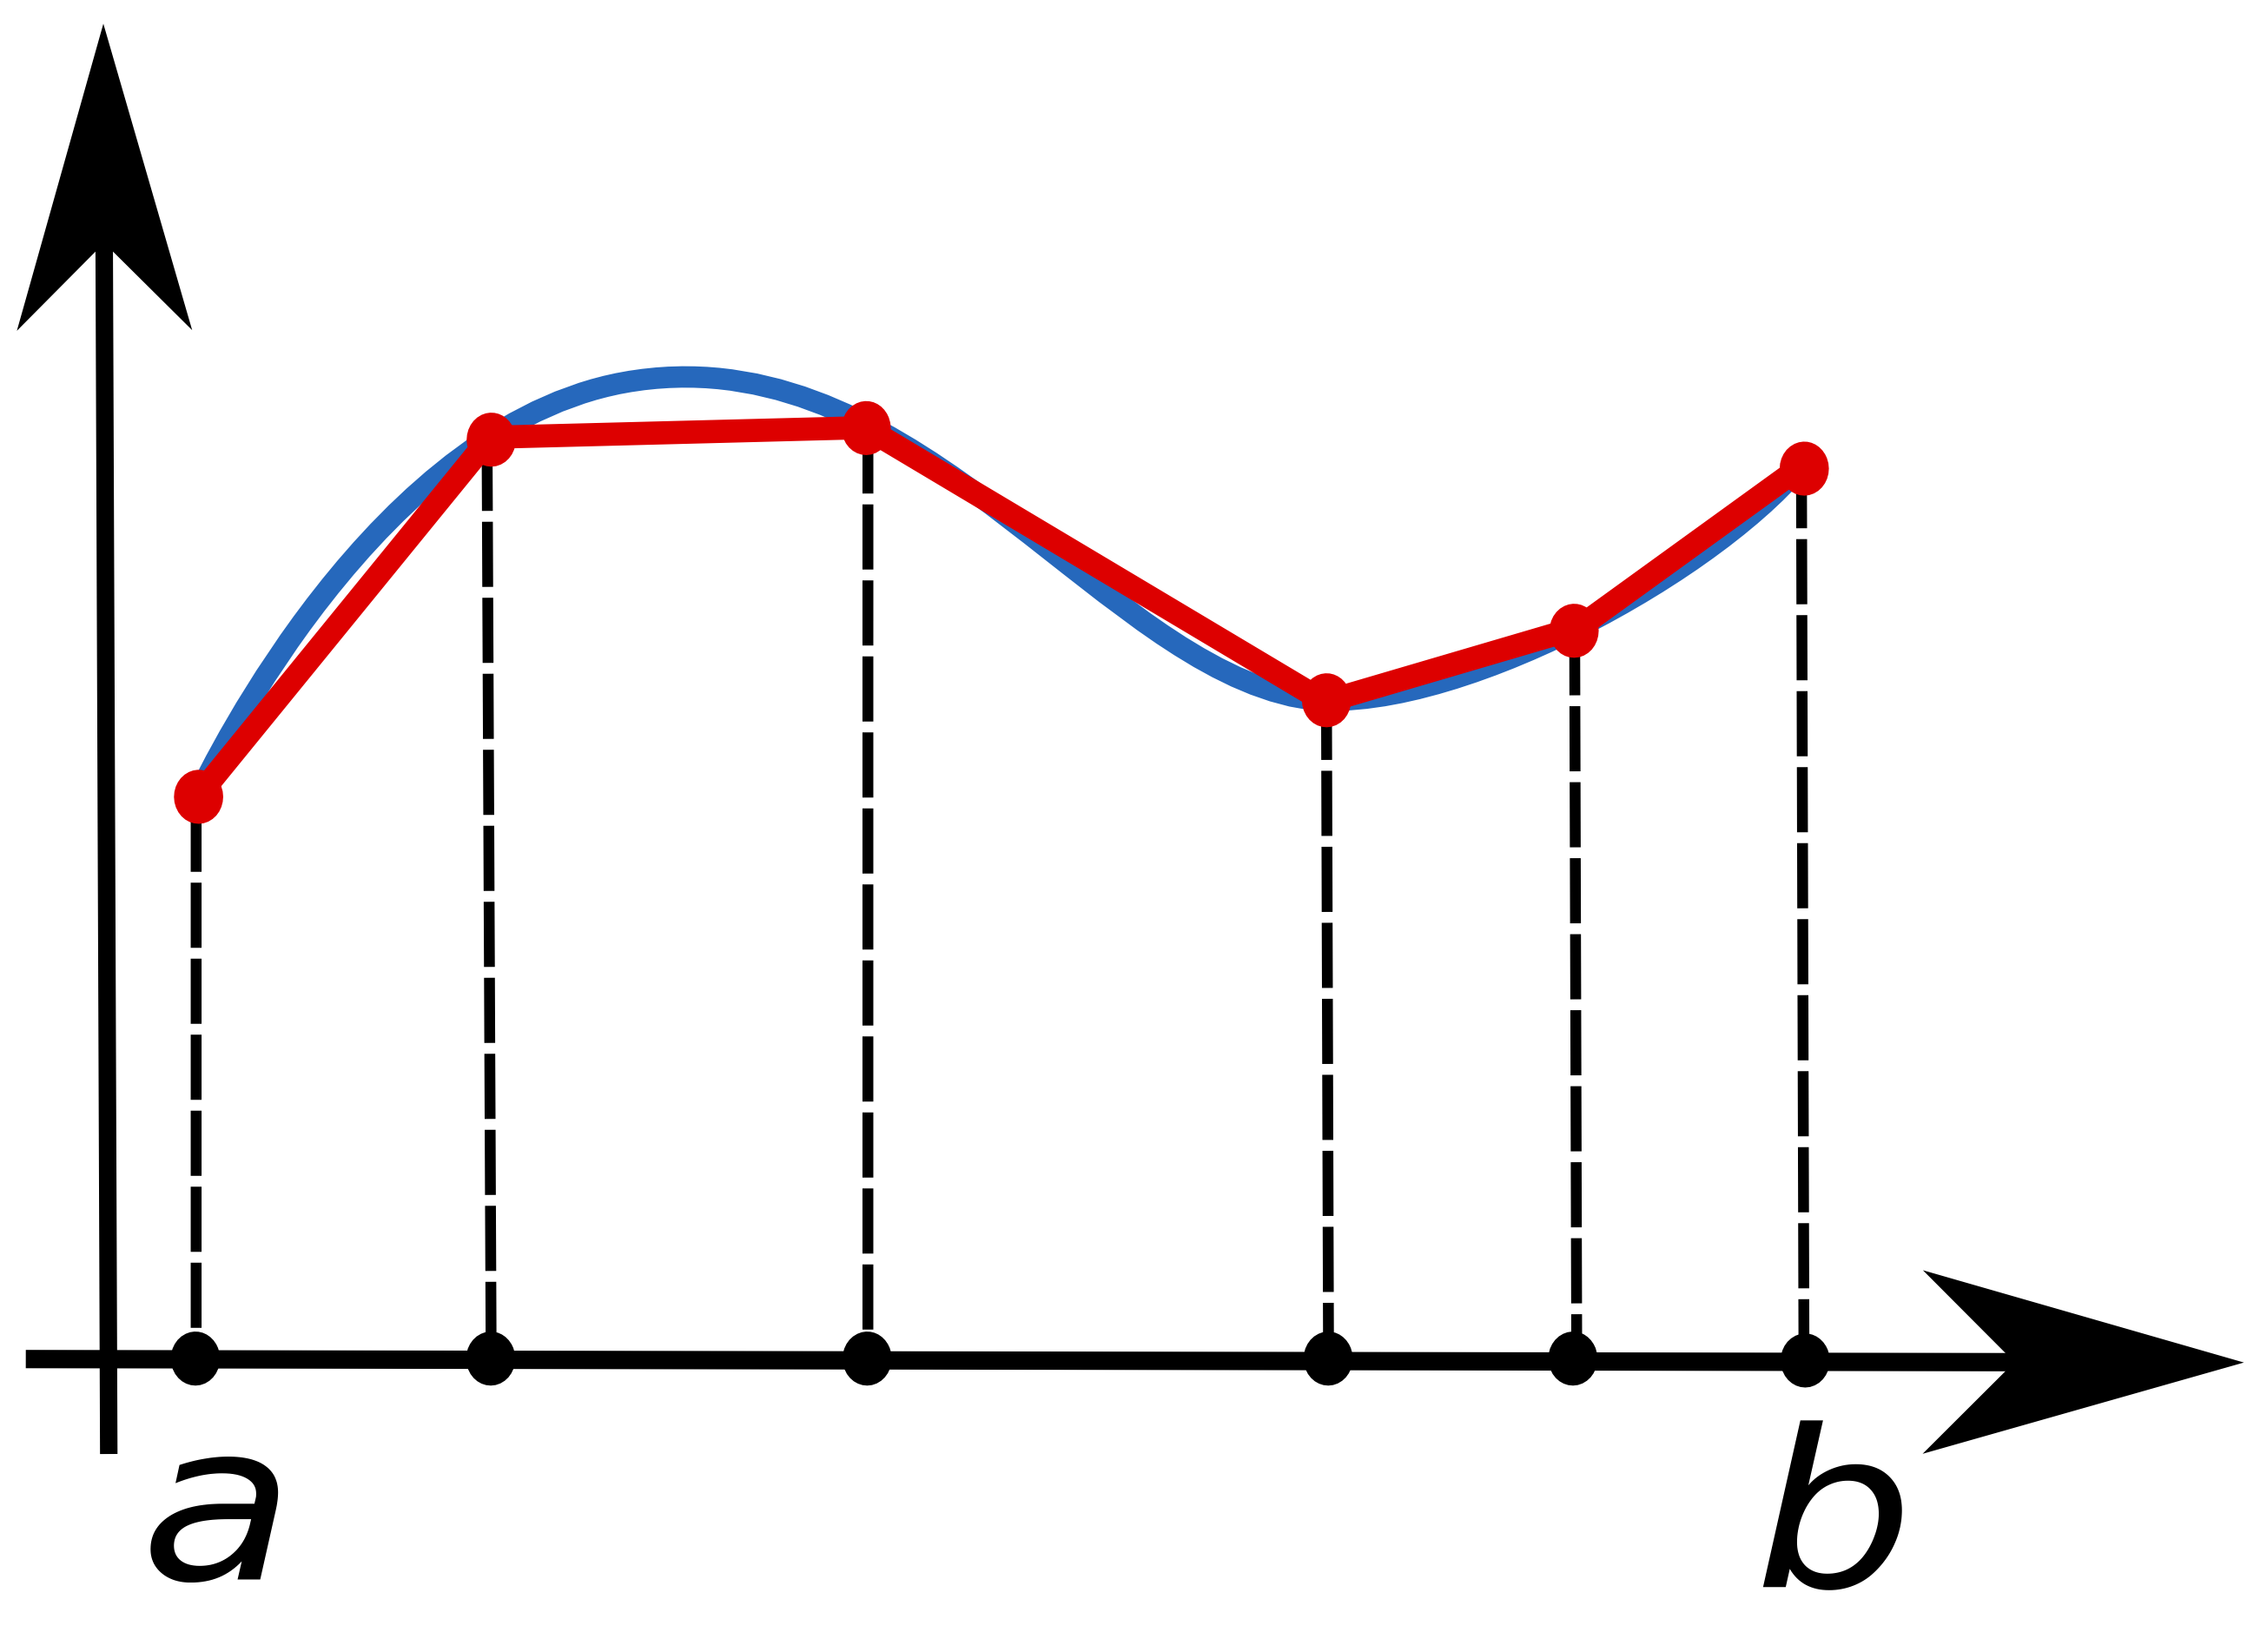
\includegraphics[width=4in]{fig/Composite_trapezoidal_rule_illustration}\par\end{centering}


\caption{\label{fig:trapezoid}Illustration of the composite trapezoidal rule
with a non-uniform grid (Image credit: Wikipedia).}
\end{figure}


Listing~\ref{code:trapezoid} contains a skeleton for this problem,
written in the form of two incomplete functions and a set of automatic
tests (in the form of \emph{unit tests}, as described in the introduction).

\lstinputlisting[label=code:trapezoid,caption={IGNORED}]{problems/trapezoid.py}

In this exercise, you'll need to write two functions, \texttt{trapz}
and \texttt{trapzf}. \texttt{trapz} applies the trapezoid formula
to pre-computed values, implementing equation~(\ref{eq:trapz}),
while \texttt{trapzf} takes a function $f$ as input, as well as the
total number of samples to evaluate, and computes eq.~(\ref{eq:trapzf2}).


\section{Newton's method}
\label{sec:quad_newton}

Consider the problem of solving for $t$ in\begin{equation}
\int_{o}^{t}f(s)ds=u\end{equation}
 where $f(s)$ is a monotonically increasing function of $s$ and
$u>0$.

This problem can be simply solved if seen as a root finding question.
Let\begin{equation}
g(t)=\int_{o}^{t}f(s)ds-u,\end{equation}
then we just need to find the root for $g(t),$ which is guaranteed
to be unique given the conditions above. 

The SciPy library includes an optimization package that contains a
Newton-Raphson solver called \texttt{scipy.optimize.newton.} This
solver can optionally take a known derivative for the function whose
roots are being sought, and in this case the derivative is simply
\begin{equation}
\frac{dg(t)}{dt}=f(t).\end{equation}


For this exercise, implement the solution for the test function\[
f(t)=t\sin^{2}(t),\]
 using \[
u=\frac{1}{4}.\]


The listing~\ref{code:quad_newton} contains a skeleton that
includes for comparison the correct numerical value.

\lstinputlisting[label=code:quad_newton,caption={IGNORED}]{examples/quad_newton.py}




\chapter{Linear algebra}
Like matlab, numpy and scipy have support for fast linear algebra
built upon the highly optimized LAPACK, BLAS and ATLAS fortran linear
algebra libraries.  Unlike Matlab, in which everything is a matrix or
vector, and the '*' operator always means matrix multiple, the default
object in numpy is an \texttt{array}, and the '*' operator on arrays means
element-wise multiplication.  

Instead, numpy provides a \texttt{matrix} class if you want to do
standard matrix-matrix multiplication with the '*' operator, or the
\texttt{dot} function if you want to do matrix multiplies with plain
arrays.  The basic linear algebra functionality is found in
\texttt{numpy.linalg}

\begin{lstlisting}
In [1]: import numpy as npy
In [2]: import numpy.linalg as linalg

# X and Y are arrays
In [3]: X = npy.random.rand(3,3)
In [4]: Y = npy.random.rand(3,3)

# * operator is element wise multiplication, not matrix matrix
In [5]: print X*Y
[[ 0.00973215  0.18086148  0.05539387]
 [ 0.00817516  0.63354021  0.2017993 ]
 [ 0.34287698  0.25788149  0.15508982]]

# the dot function will use optimized LAPACK to do matrix-matix
# multiply
In [6]: print npy.dot(X, Y)
[[ 0.10670678  0.68340331  0.39236388]
 [ 0.27840642  1.14561885  0.62192324]
 [ 0.48192134  1.32314856  0.51188578]]

# the matrix class will create matrix objects that support matrix
# multiplication with *
In [7]: Xm = npy.matrix(X)
In [8]: Ym = npy.matrix(Y)
In [9]: print Xm*Ym
[[ 0.10670678  0.68340331  0.39236388]
 [ 0.27840642  1.14561885  0.62192324]
 [ 0.48192134  1.32314856  0.51188578]]

# the linalg module provides functions to compute eigenvalues,
# determinants, etc.  See help(linalg) for more info
In [10]: print linalg.eigvals(X)
[ 1.46131600+0.j          0.46329211+0.16501143j  0.46329211-0.16501143j]

\end{lstlisting}

\section{Glass Moir\'e Patterns}
\label{sec:glass_patterns}

When a random dot pattern is scaled, rotated, and superimposed over
the original dots, interesting visual patterns known as Glass Patterns
emerge\footnote{L. Glass. 'Moir\'e effect from random dots' Nature 223,
  578580 (1969).}  In this exercise, we generate random dot fields
using numpy's uniform distribution function, and apply
transformations to the random dot field using a scale $\mathbf{S}$
and rotation $\mathbf{R}$ matrix $\mathbf{X_2} = \mathbf{S} \mathbf{R}
\mathbf{X_1}$.

If the scale and rotation factors are small, the transformation is
analogous to a single step in the numerical solution of a 2D ODE, and
the plot of both $\mathbf{X_1}$ and $\mathbf{X_2}$ will reveal the
structure of the vecotr field flow around the fixed point (the
invariant under the transformation); see for example the
\textit{stable focus}, aka \textit{spiral}, in
Figure~\ref{fig:glass_dots1}.

The eigenvalues of the tranformation matrix $\mathbf{M} =
\mathbf{S}\mathbf{R}$ determine the type of fix point:
\textit{center}, \textit{stable focus}, \textit{saddle node},
etc\dots.  For example, if the two eigenvalues are real but differing
in signs, the fixed point is a \textit{saddle node}.  If the real
parts of both eigenvalues are negative and the eigenvalues are
complex, the fixed point is a \textit{stable focus}.  The complex part
of the eigenvalue determines whether there is any rotation in the
matrix transformation, so another way to look at this is to break out
the scaling and rotation components of the transformation
$\textbf{M}$.  If there is a rotation component, then the fixed point
will be a \textit{center} or a \textit{focus}.  If the scaling
components are both one, the rotation will be a \textit{center}, if
they are both less than one (contraction), it will be a \textit{stable
  focus}.  Likewise, if there is no rotation component, the fixed
point will be a \textit{node}, and the scaling components will
determine the type of node.  If both are less than one, we have a
\textit{stable node}, if one is greater than one and the other less
than one, we have a \textit{saddle node}.

\lstinputlisting[label=code:glass_dots1,caption={IGNORED}]{examples/glass_dots1.py}



\begin{center}%
\begin{figure}
\begin{centering}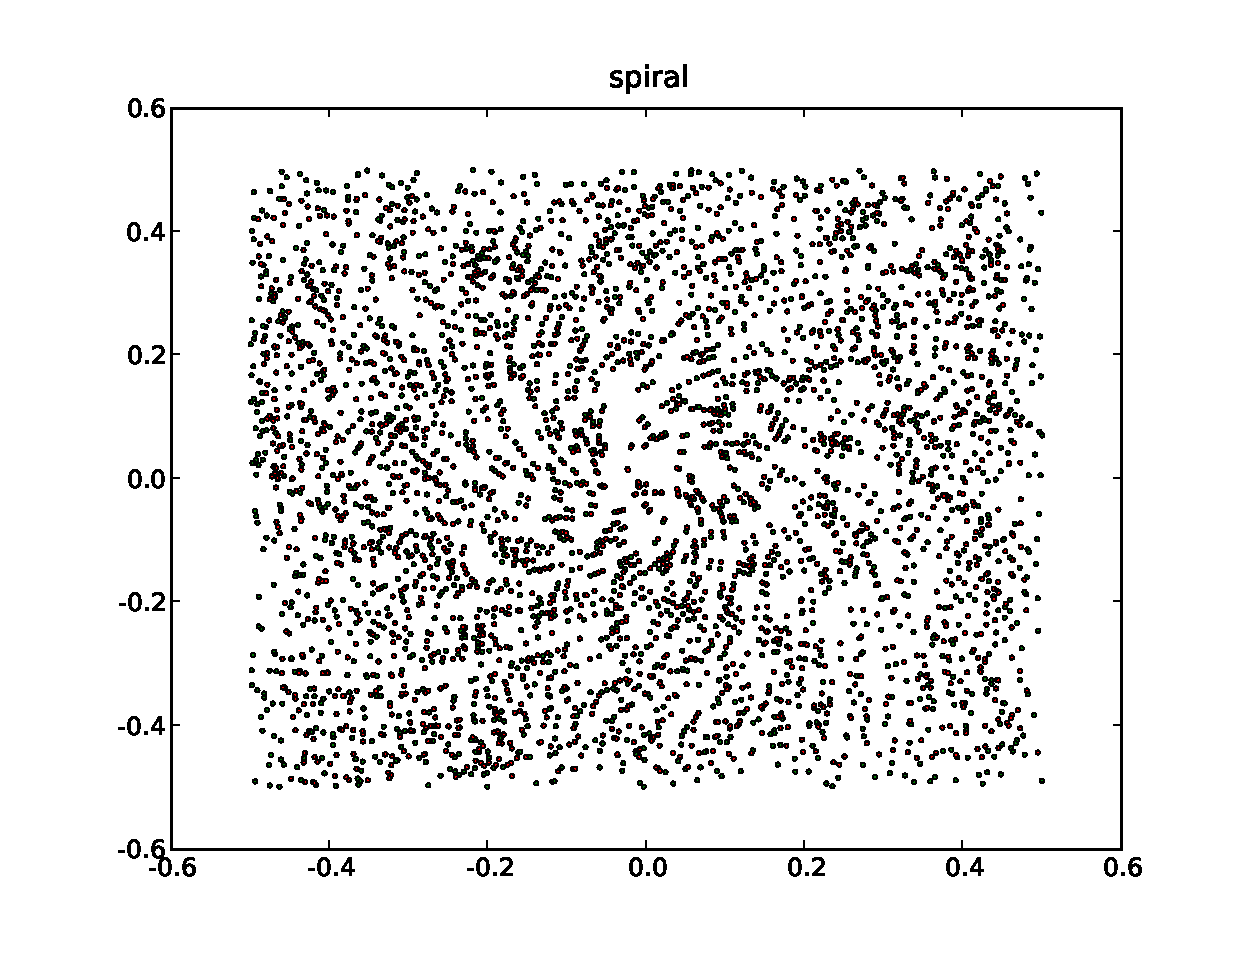
\includegraphics[width=4in]{fig/glass_dots1}\par\end{centering}


\caption{\label{fig:glass_dots1}Glass pattern showing a stable focus}
\end{figure}
\par\end{center}


\chapter{Signal processing}
\texttt{numpy} and \texttt{scipy} provide many of the essential tools
for digital signal processing.  \texttt{scipy.signal} provides basic
tools for digital filter design and filtering (eg Butterworth
filters), a linear systems toolkit, standard waveforms such as square
waves, and saw tooth functions, and some basic wavelet functionality.
\texttt{scipy.fftpack} provides a suite of tools for Fourier domain
analysis, including 1D, 2D, and ND discrete fourier transform and
inverse functions, in addition to other tools such as analytic signal
representations via the Hilbert trasformation (\texttt{numpy.fft} also
provides basic FFT functions).  \texttt{pylab} provides Matlab
compatible functions for computing and plotting standard time series
analyses, such as historgrams (\texttt{hist}), auto and cross
correlations (\texttt{acorr} and \texttt{xcorr}), power spectra and
coherence spectra (\texttt{psd}, \texttt{csd}, \texttt{cohere} and
\texttt{specgram}).  



\begin{center}%
\begin{figure}
\begin{centering}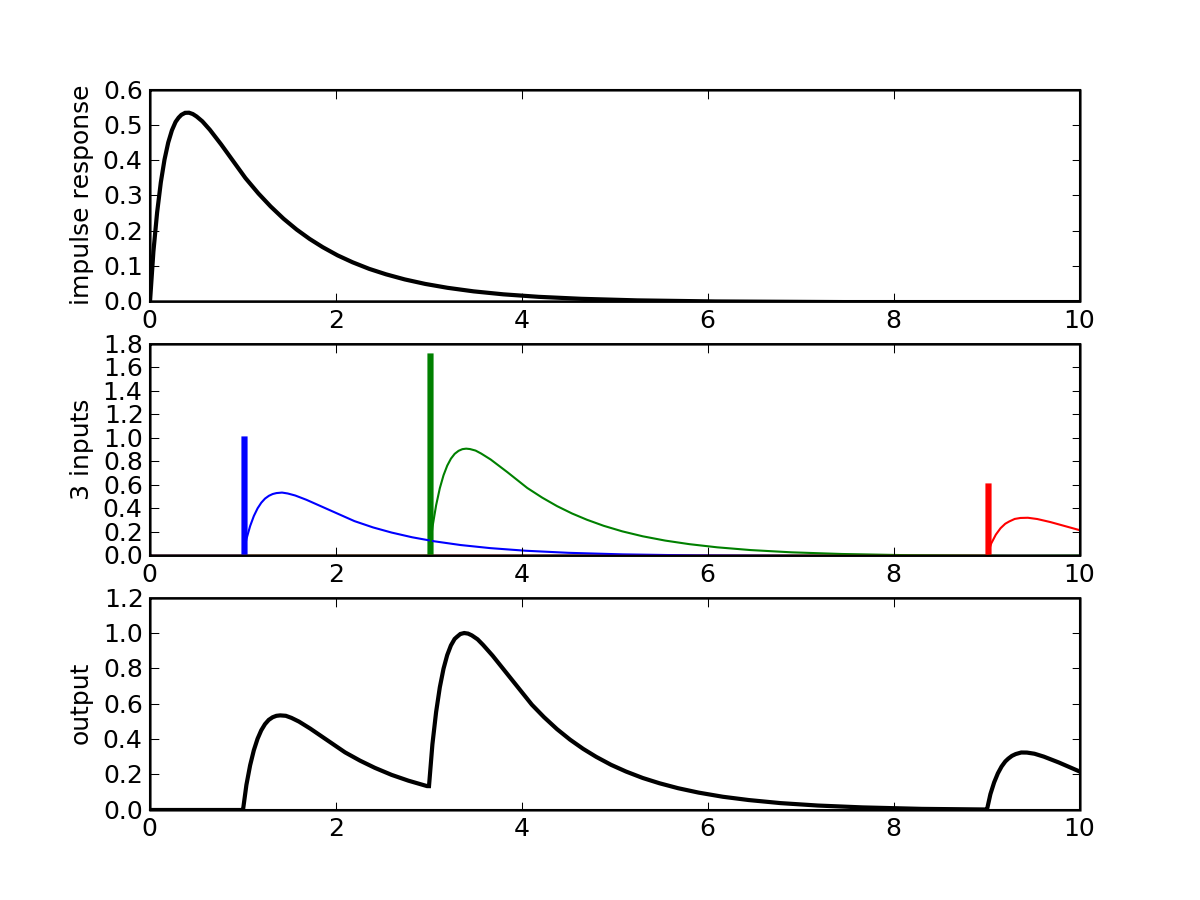
\includegraphics[width=4in]{fig/convolve_explain}\par\end{centering}
\caption{\label{fig:convolve_explain}The output of a linear system to a series of impulse inputs is equal to the sum of the scaled and time shifted impulse response functions.}
\end{figure}
\par\end{center}

\begin{center}%
\begin{figure}
\begin{centering}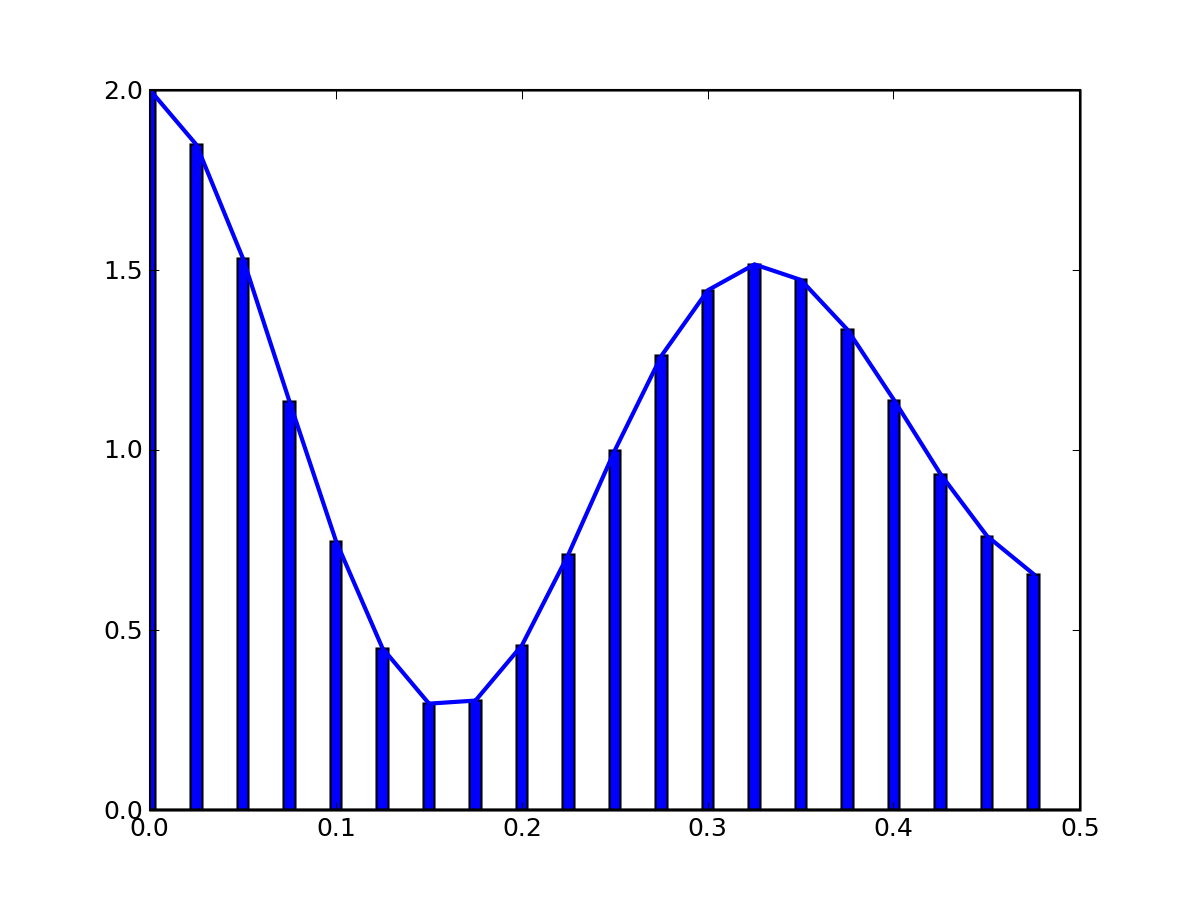
\includegraphics[width=4in]{fig/convolve_deltas}\par\end{centering}
\caption{\label{fig:convolve_deltas}Representing a continuous time signal sampled as a sum of delta functions.}
\end{figure}
\par\end{center}


\lstinputlisting[label=code:convolution_demo,caption={IGNORED}]{skel/convolution_demo_skel.py}



\begin{center}%
\begin{figure}
\begin{centering}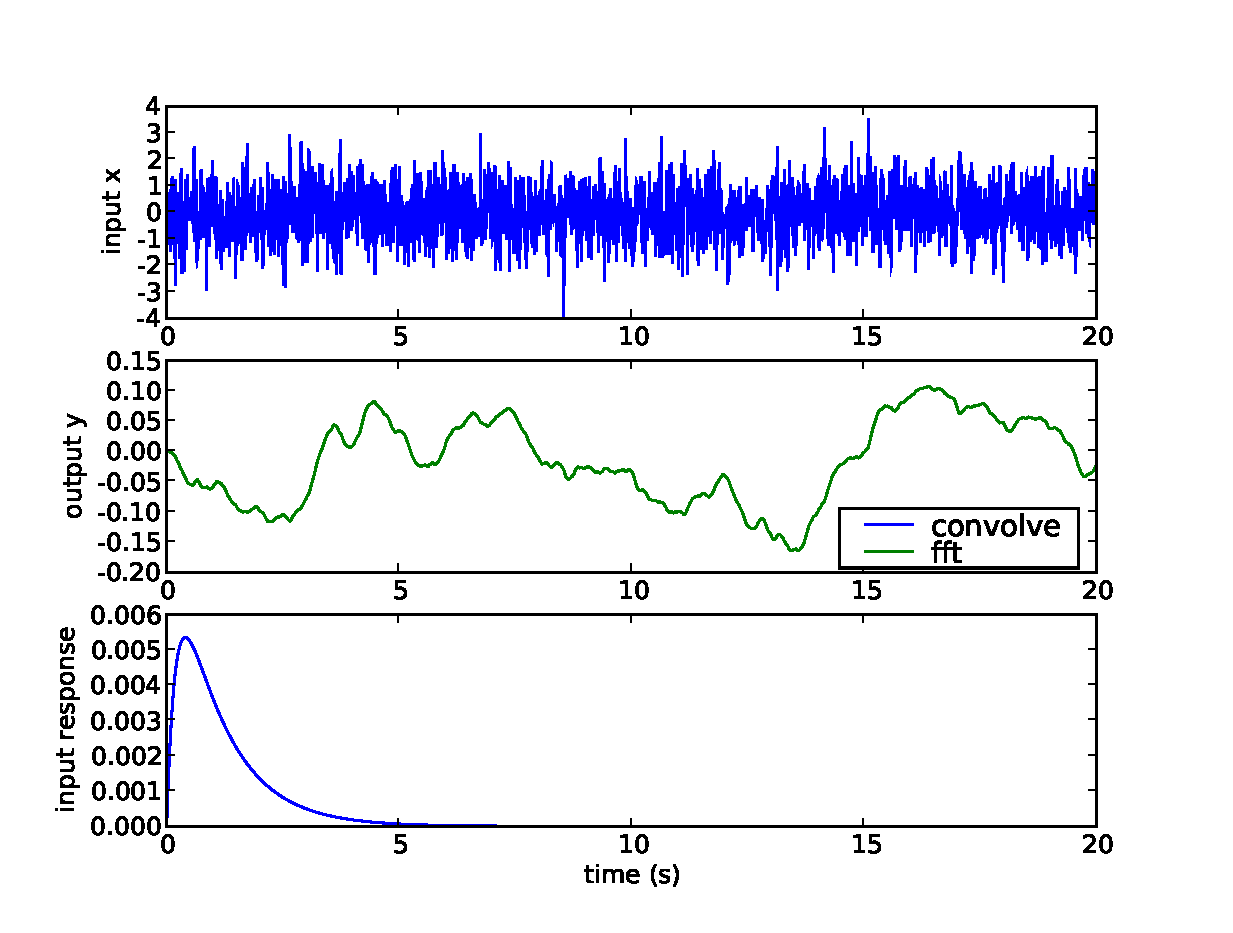
\includegraphics[width=4in]{fig/convolution_demo}\par\end{centering}
\caption{\label{fig:convolution_demo}Convolution of a white noise process with a double exponential function computed with \texttt{numpy.fft} and \texttt{numpy.convolve}}
\end{figure}
\par\end{center}

\section{FFT Image Denoising}
\label{sec:fft_imdenoise}

\textbf{Illustrates}: 2-d image denoising, use of the scipy FFT library,
array manipulations, image plotting.

Convolution of an input with with a linear filter in the termporal or spatial
domain is equivalent to multiplication by the fourier transforms of the input
and the filter in the spectral domain.  This provides a conceptually simple way
to think about filtering: transform your signal into the frequency domain,
dampen the frequencies you are not interested in by multiplying the frequency
spectrum by the desired weights, and then apply the inverse transform to the
modified spectrum, back into the original domain.  In the example below, we
will simply set the weights of the frequencies we are uninterested in (the high
frequency noise) to zero rather than dampening them with a smoothly varying
function.  Although this is not usually the best thing to do, since sharp edges
in one domain usually introduce artifacts in another (eg high frequency
``ringing''), it is easy to do and sometimes provides satisfactory results.

The image in the upper left panel of Figure~\ref{fig:fft_imdenoise} is a
grayscale photo of the moon landing.  There is a banded pattern of high
frequency noise polluting the image.  In the upper right panel we see the 2D
spatial frequency spectrum.  The FFT output in \texttt{scipy} is packed with
the lower freqeuencies starting in the upper left, and proceeding to higher
frequencies as one moves to the center of the spectrum (this is the most
efficient way numerically to fill the output of the FFT algorithm).  Because
the input signal is real, the output spectrum is complex and symmetrical: the
transformation values beyond the midpoint of the frequency spectrum (the
Nyquist frequency) correspond to the values for negative frequencies and are
simply the mirror image of the positive frequencies below the Nyquist (this is
true for the 1D, 2D and ND FFTs in \texttt{numpy}).

In this exercise we will compute the 2D spatial frequency spectra of the
luminance image, zero out the high frequency components, and inverse transform
back into the spatial domain.  We can plot the input and output images with the
\texttt{pylab.imshow} function, but the images must first be scaled to be
within the 0..1 luminance range.  For best results, it helps to
\textit{amplify} the image by some scale factor, and then \textit{clip} it to
set all values greater than one to one.  This serves to enhance contrast among
the darker elements of the image, so it is not completely dominated by the
brighter segments

\lstinputlisting[label=code:fft_imdenoise,caption={IGNORED}]{problems/fft_imdenoise.py}

\begin{figure}
  \begin{centering} 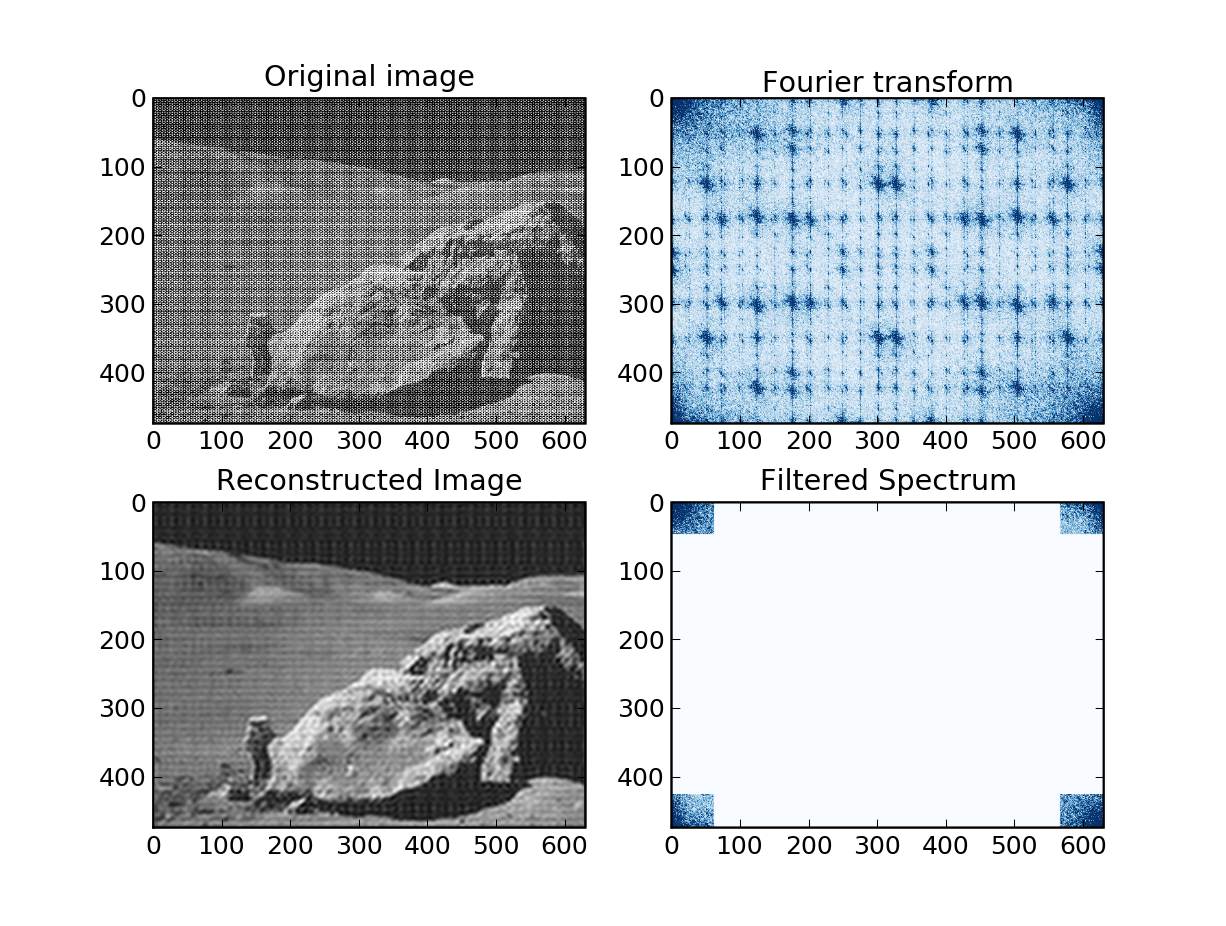
\includegraphics[width=4in]{fig/fft_imdenoise} \par
  \end{centering}

  \caption{\label{fig:fft_imdenoise}High freqeuency noise filtering of a 2D
    image in the Fourier domain.  The upper panels show the original image
    (left) and spectral power (right) and the lower panels show the same data
    with the high frequency power set to zero.  Although the input and output
    images are grayscale, you can provide colormaps to \texttt{pylab.imshow} to
    plot them in psudo-color}
\end{figure}


\chapter{Dynamical Systems}
TODO
\section{Lotka-Volterra Equations}
\label{sec:lotka_volterra}

\lstinputlisting[label=code:lotka_volterra_skel,caption={IGNORED}]{skel/lotka_volterra_skel.py}

\begin{figure}
\begin{centering}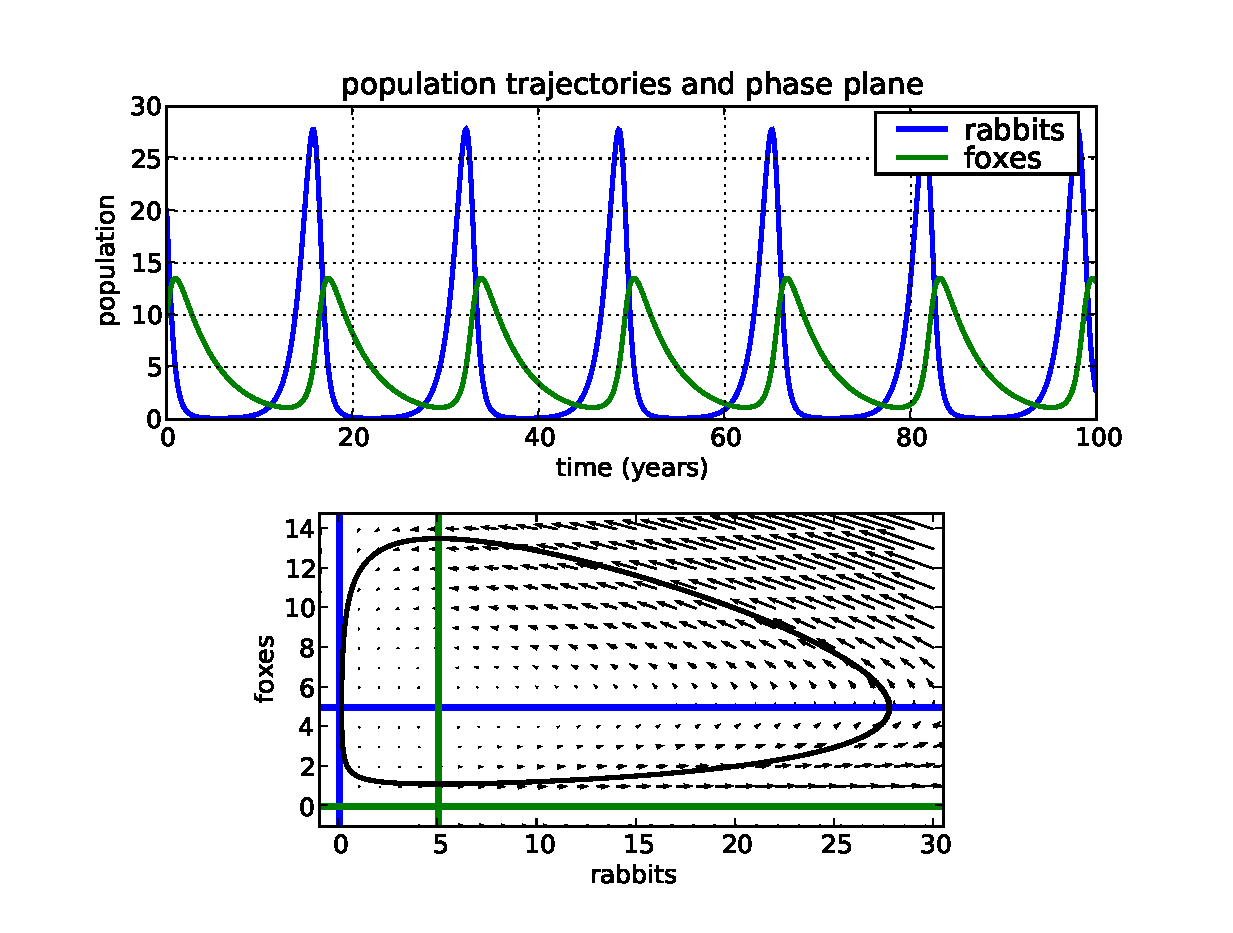
\includegraphics[width=3in]{fig/lotka_volterra}\par\end{centering}

\caption{\label{fig:lotka_volterra}Upper panel shows population
  trajectories for rabbits (blue) and foxes (green) simulated using
  the Lotka-Volterra population dynamics equations.  Lower panel shows
  the phase-plane trajectories, direction field and nullclines.}
\end{figure}


\chapter{Statistics}
TODO
\section{Descriptive statistics}
\label{sec:stats_descriptives}


\lstinputlisting[label=code:stats_descriptives_skel,caption={IGNORED}]{skel/stats_descriptives_skel.py}

\begin{figure}
\begin{centering}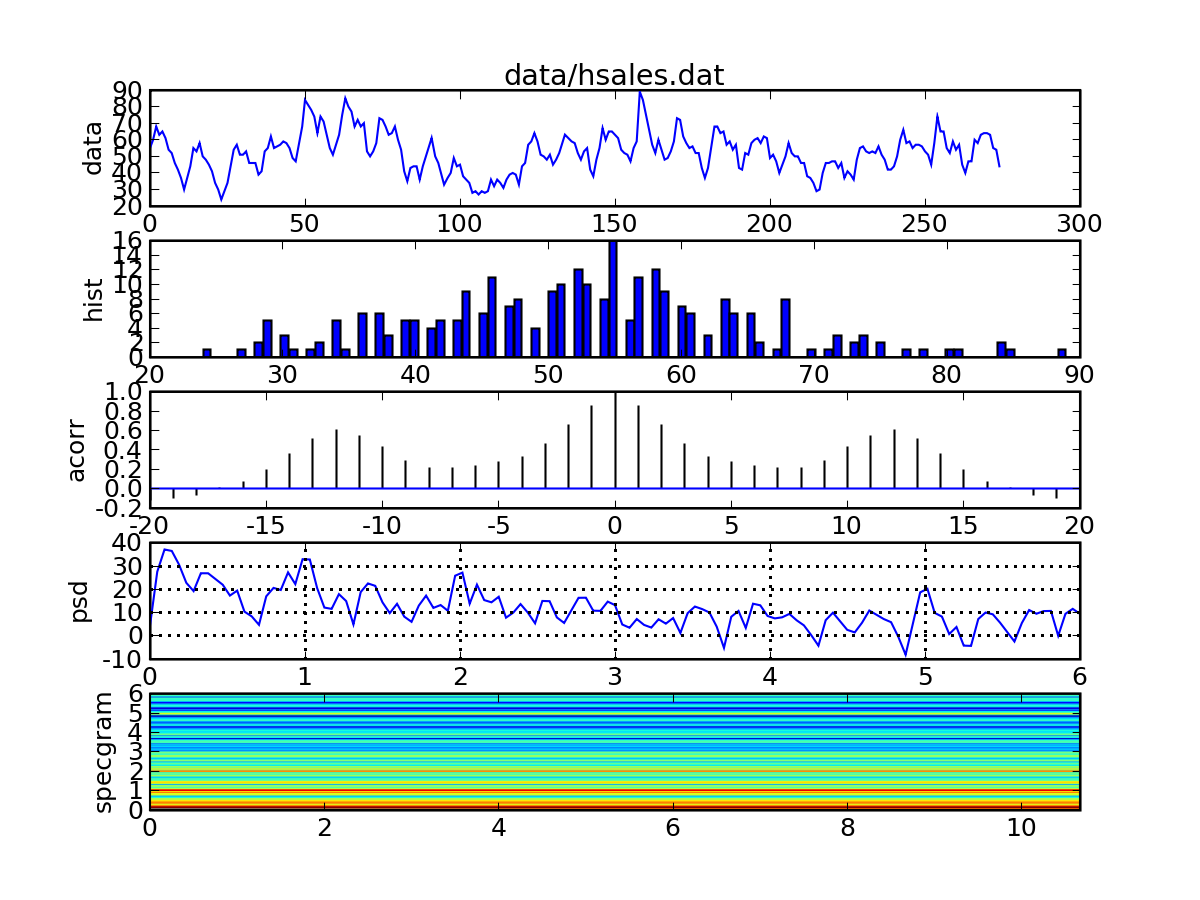
\includegraphics[width=3in]{fig/stats_descriptives}\par\end{centering}

\caption{\label{fig:stats_descriptives}}
\end{figure}

\section{Statistical distributions}
\label{sec:stats_distributions}

We explore a handful of the statistical distributions in
\texttt{scipy.stats} module and the connections between them.  The
organization of the distribution functions in \texttt{scipy.stats} is
quite elegant, with each distribution providing random variates
(\texttt{rvs}), analytical moments (mean, variance, skew, kurtosis),
analytic density (\texttt{pdf}, \texttt{cdf}) and survival functions
(\texttt{sf}, \textt{isf}) (where available) and tools for fitting
empirical distributions to the analytic distributions (\textt{fit}).

in the exercise below, we will simulate a radioactive particle
emitter, and look at the empirical distribution of waiting times
compared with the expected analytical distributions.  Our radioative
particle emitter has an equal likelihood of emitting a particle in any
equal time interval, and emits particles at a rate of 20~Hz.  We will
discretely sample time at a high frequency, and record a 1 of a
particle is emitted and a 0 otherwise, and then look at the
distribution of waiting times between emissions.  The probability of a
particle emission in one of our sample intervals (assumed to be very
small compared to the average interval between emissions) is
proportional to the rate and the sample interval $\Delta t$, ie
$p(\Delta t) = \alpha \Delta t$ where $\alpha$ is the emission rate in
particles per second.

\begin{lstlisting}

# a uniform distribution [0..1]
In [62]: uniform = scipy.stats.uniform()

# our sample interval in seconds
In [63]: deltat = 0.001

# the emission rate, 20Hz
In [65]: alpha = 20

# 1000 random numbers
In [66]: rvs = uniform.rvs(1000)

# a look at the 1st 20 random variates
In [67]: rvs[:20]
Out[67]: 
array([ 0.71167172,  0.01723161,  0.25849255,  0.00599207,  0.58656146,
        0.12765225,  0.17898621,  0.77724693,  0.18042977,  0.91935639,
        0.97659579,  0.59045477,  0.94730366,  0.00764026,  0.12153159,
        0.82286929,  0.18990484,  0.34608396,  0.63931108,  0.57199175])

# we simulate an emission when the random number is less than
# p(Delta t) = alpha * deltat
In [84]: emit = rvs < (alpha * deltat)


# there were 3 emissions in the first 20 observations
In [85]: emit[:20]
Out[85]: 
array([False,  True, False,  True, False, False, False, False, False,
       False, False, False, False,  True, False, False, False, False,
       False, False], dtype=bool)
\end{lstlisting}

The waiting times between the emissions should follow an exponential
distribution (see \texttt{scipy.stats.expon}) with a mean of
$1/\alpha$.  In the exercise below, you will generate a long array of
emissions, compute the waiting times between emissions, between 2
emissions, and between 10 emissions.  These should approach an 1st
order gamma (aka exponential) distribution, 2nd order gamma, and 10th
order gamma (see \texttt{scipy.stats.gamma}).  Use the probability
density functions for these distributions in \texttt{scipy.stats} to
compare your simulated distributions and moments with the analytic
versions provided by \texttt{scipy.stats}.  With 10 waiting times, we
should be approaching a normal distribution since we are summing 10
waiting times and under the central limit theorem the sum of
independent samples from a finite variance process approaches the
normal distribution (see \texttt{scipy.stats.norm}).  In the final
part of the exercise below, you will be asked to approximate the 10th
order gamma distribution with a normal distribution.  The results
should look something like those in
Figure~\ref{fig:stats_distributions}.

\lstinputlisting[label=code:stats_distributions_skel,caption={IGNORED}]{skel/stats_distributions_skel.py}

\begin{figure}
\begin{centering}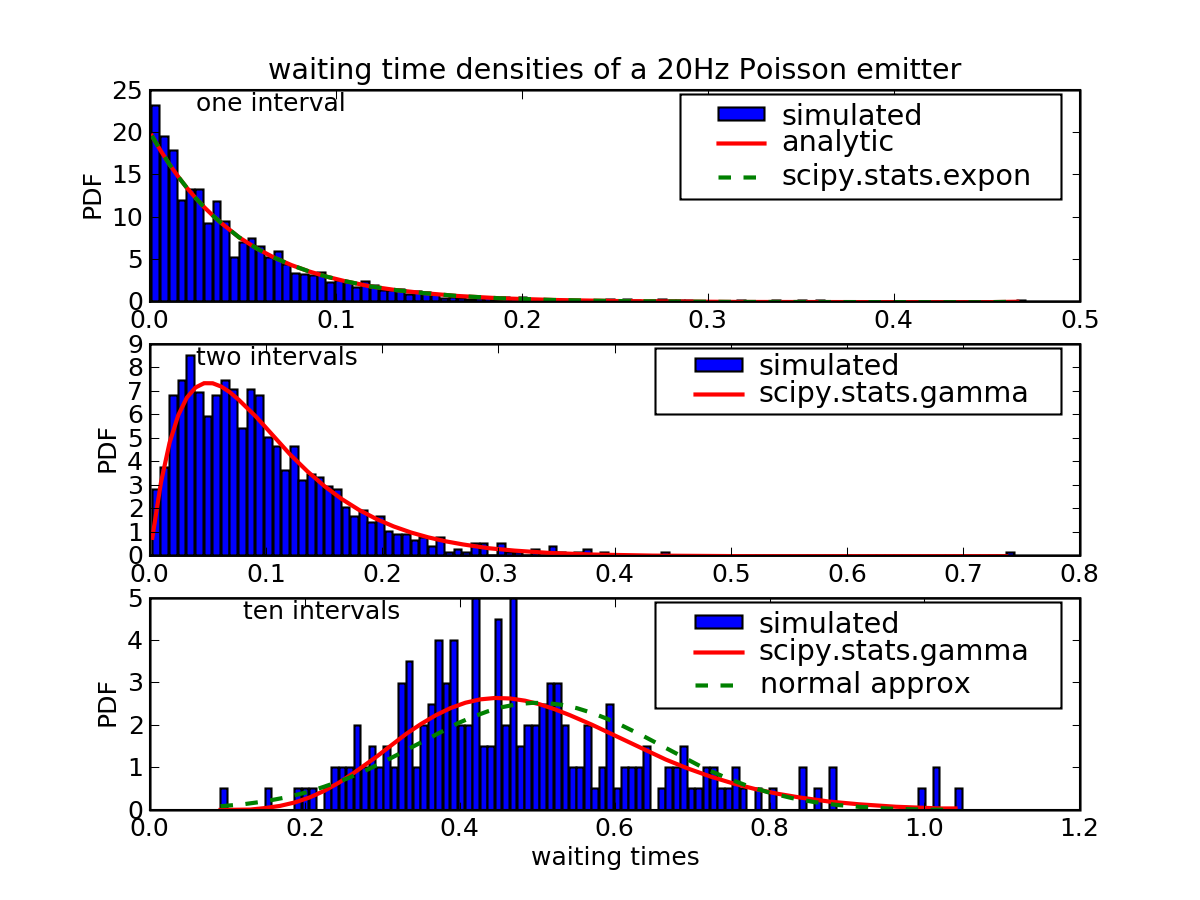
\includegraphics[width=3in]{fig/stats_distributions}\par\end{centering}

\caption{\label{fig:stats_distributions}}
\end{figure}


\chapter{Plotting on Maps}
The matplotlib basemap toolkit is an add-on for matplotlib that provides
the capability to draw maps of the earth in various map projections,
and plot data on those maps. This section shows how to use basemap
to create simple maps, draw coastlines and political boundaries, draw
lines of constant latitude and longitude, and plot geophysical data
on the maps.


\section{Setting up the map.}

In order to represent the curved surface of the earth in a two-dimensional
map, a map projection is needed. Since this cannot be done without
distortion, there are many map projections, each with it's own advantages
and disadvantages. Basemap provides 19 different map projections.
Some are global, some can only represent a portion of the globe. When
a Basemap class instance is created, the desired map projection must
be specified, along with information about the portion of the earth's
surface that the map projection will describe. There are two basic
ways of doing this. One is to provide the latitude and longitude values
of each of the four corners of the rectangular map projection region.
The other is to provide the lat/lon value of the center of the map
projection region along with the width and height of the region in
map projection coordinates. The first script illustrates how to use
both of these methods to create a simple map. It also shows how to
draw the continents and political boundaries on the map.

Here is an example script that creates a map by specifying the latitudes
and longitudes of the four corners

\lstinputlisting[label=code:basemap1_skel,caption={IGNORED}]{../examples/basemap1.py}

After running this script, you should see a plot that looks similar
to Figure 1.

\begin{figure}[h]
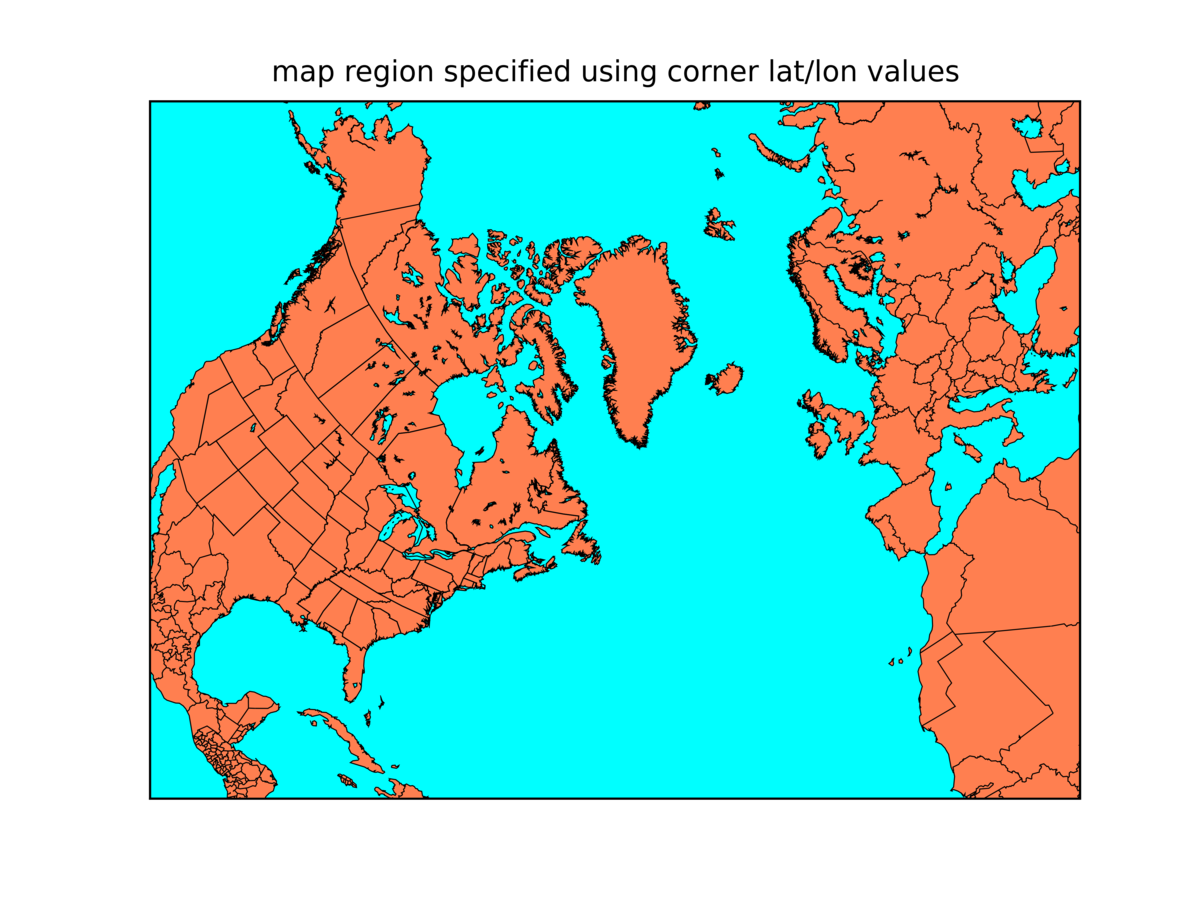
\includegraphics[scale=0.75]{fig/basemap1}

\caption{A map created by specifying the latitudes and longitudes of the four
corners.}

\end{figure}

\medskip{}
Here is an example script that creates a map by specifying the center
of the map, plus the width and height in meters.

\lstinputlisting[label=code:basemap2_skel,caption={IGNORED}]{../examples/basemap2.py}

After running this script, you should see a plot that looks nearly
identical to Figure 1.\medskip{}


The Basemap class instance can be used to convert latitudes and longitudes
to coordinates on the map. To do this, simply call the instance as
if it were a function, passing it the longitude and latitudes values
to convert. The corresponding x and y values in map projection coordinates
will be returned. The following example script shows how to use this
to plot the locations of two cities (New York and London). The Basemap
method drawgreatcircle is then used to draw the great circle route
between these cities on the map.

\lstinputlisting[label=code:basemap3_skel,caption={IGNORED}]{../examples/basemap3.py}

This should produce something similar to Figure 2.

\begin{figure}[h]
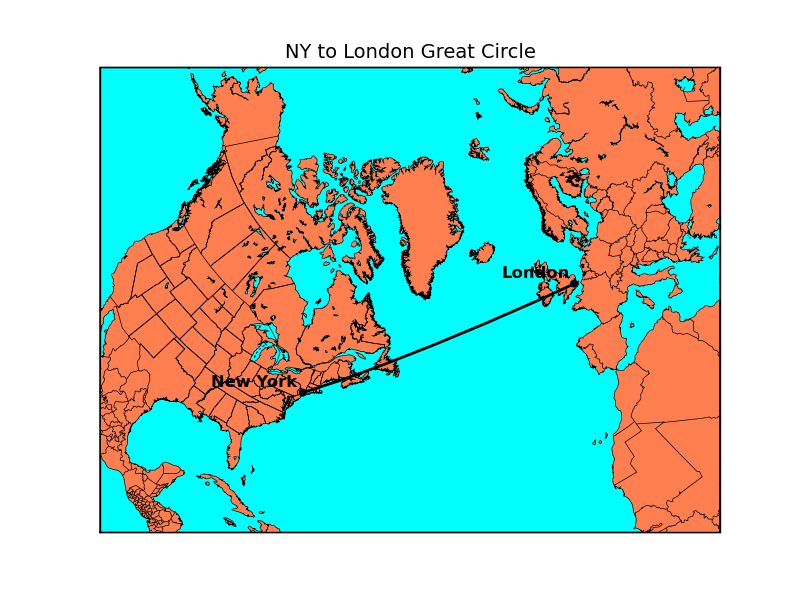
\includegraphics[scale=0.75]{fig/basemap3}

\caption{Drawing the locations of two cities, and connecting them along a great
circle.}

\end{figure}

\medskip{}
Most maps include a graticule grid, a reference network of labelled
latitude and longitude lines. Basemap does this with the drawparallels
and drawmeridians instance methods. The longitude and latitude lines
can be labelled where the intersect the map projection boundary. Following
is an example script that draws a graticule on the map we've been
working with.

\lstinputlisting[label=code:basemap4_skel,caption={IGNORED}]{../examples/basemap4.py}

Running this script should produce a plot that looks like Figure 3.

\begin{figure}[h]
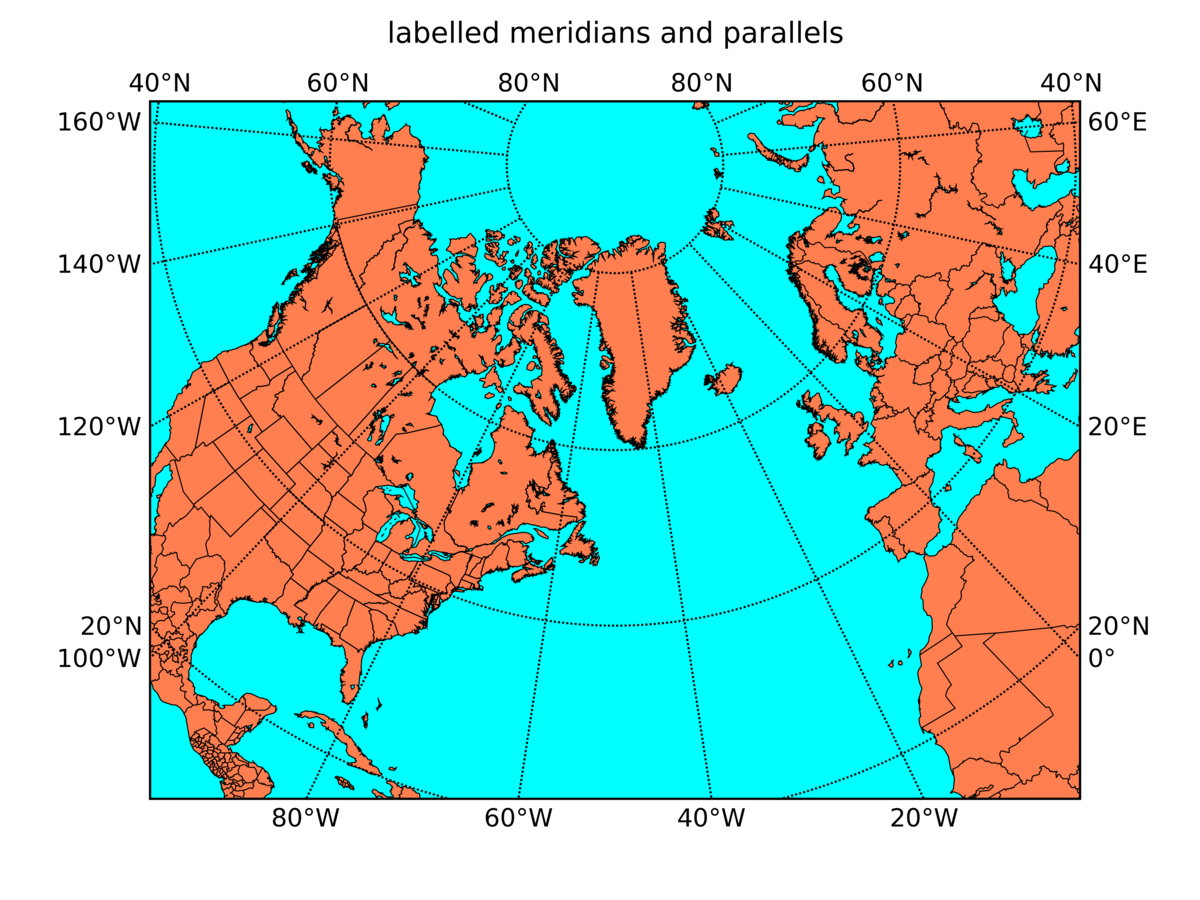
\includegraphics[scale=0.75]{fig/basemap4}

\caption{Drawing labelled meridians and parallels on the map (a graticule grid).}

\end{figure}


\section{Plotting geophysical data on the map.}

One of the most common uses of Basemap is to visualize earth science
data, such as output from climate models. These data often come on
latitude/longitude grids. One common data format for storing such
grids is NetCDF. Basemap includes a NetCDF file reader (written in
pure python by Roberto D'Almeida). There are python packages available
for reading just about every other scientific data format imaginable,
including HDF, GRIB, FITS and many others. Following is an example
of how to read sea-surface temperature data from a NetCDF file and
plot it on a global mollweide projection.

\lstinputlisting[label=code:basemap5_skel,caption={IGNORED}]{../examples/basemap5.py}

The resulting plot should look like Figure 4.

\pagebreak

\begin{figure}[h]
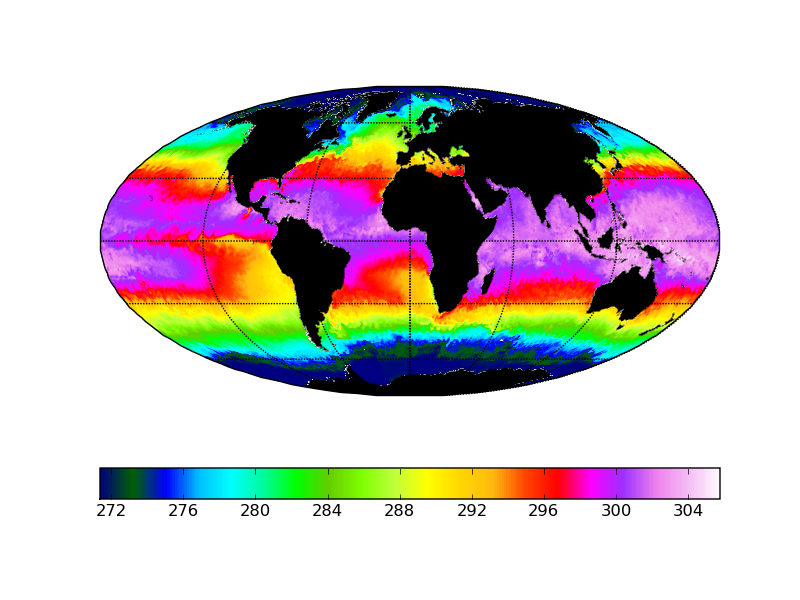
\includegraphics[scale=0.75]{fig/basemap5}

\caption{Sea surface temperature on a global mollweide projection.}

\end{figure}

\medskip{}

Basemap also is capable of reading ESRI shapefiles, a very common
GIS format. The script fillstates.py in the examples directory of
the basemap source distribution shows how to read and plot polygons
in a shapefile. There are many other useful examples in that directory
that illustrate various ways of using basemap.%


\bibliographystyle{plain}
\bibliography{python,python2}

\end{document}
